% Options for packages loaded elsewhere
\PassOptionsToPackage{unicode}{hyperref}
\PassOptionsToPackage{hyphens}{url}
\PassOptionsToPackage{dvipsnames,svgnames,x11names}{xcolor}
%
\documentclass[
  12pt,
]{book}
\title{Rのすゝめ}
\usepackage{etoolbox}
\makeatletter
\providecommand{\subtitle}[1]{% add subtitle to \maketitle
  \apptocmd{\@title}{\par {\large #1 \par}}{}{}
}
\makeatother
\subtitle{〜 Rによるデータ分析事始め 〜}
\author{Sampo Suzuki, CC 4.0 BY-NC-SA}
\date{2022-03-03}

\usepackage{amsmath,amssymb}
\usepackage{lmodern}
\usepackage{setspace}
\usepackage{iftex}
\ifPDFTeX
  \usepackage[T1]{fontenc}
  \usepackage[utf8]{inputenc}
  \usepackage{textcomp} % provide euro and other symbols
\else % if luatex or xetex
  \usepackage{unicode-math}
  \defaultfontfeatures{Scale=MatchLowercase}
  \defaultfontfeatures[\rmfamily]{Ligatures=TeX,Scale=1}
\fi
% Use upquote if available, for straight quotes in verbatim environments
\IfFileExists{upquote.sty}{\usepackage{upquote}}{}
\IfFileExists{microtype.sty}{% use microtype if available
  \usepackage[]{microtype}
  \UseMicrotypeSet[protrusion]{basicmath} % disable protrusion for tt fonts
}{}
\makeatletter
\@ifundefined{KOMAClassName}{% if non-KOMA class
  \IfFileExists{parskip.sty}{%
    \usepackage{parskip}
  }{% else
    \setlength{\parindent}{0pt}
    \setlength{\parskip}{6pt plus 2pt minus 1pt}}
}{% if KOMA class
  \KOMAoptions{parskip=half}}
\makeatother
\usepackage{xcolor}
\IfFileExists{xurl.sty}{\usepackage{xurl}}{} % add URL line breaks if available
\IfFileExists{bookmark.sty}{\usepackage{bookmark}}{\usepackage{hyperref}}
\hypersetup{
  pdftitle={Rのすゝめ},
  pdfauthor={Sampo Suzuki, CC 4.0 BY-NC-SA},
  colorlinks=true,
  linkcolor={Maroon},
  filecolor={Maroon},
  citecolor={Blue},
  urlcolor={Blue},
  pdfcreator={LaTeX via pandoc}}
\urlstyle{same} % disable monospaced font for URLs
\usepackage{color}
\usepackage{fancyvrb}
\newcommand{\VerbBar}{|}
\newcommand{\VERB}{\Verb[commandchars=\\\{\}]}
\DefineVerbatimEnvironment{Highlighting}{Verbatim}{commandchars=\\\{\}}
% Add ',fontsize=\small' for more characters per line
\usepackage{framed}
\definecolor{shadecolor}{RGB}{248,248,248}
\newenvironment{Shaded}{\begin{snugshade}}{\end{snugshade}}
\newcommand{\AlertTok}[1]{\textcolor[rgb]{0.94,0.16,0.16}{#1}}
\newcommand{\AnnotationTok}[1]{\textcolor[rgb]{0.56,0.35,0.01}{\textbf{\textit{#1}}}}
\newcommand{\AttributeTok}[1]{\textcolor[rgb]{0.77,0.63,0.00}{#1}}
\newcommand{\BaseNTok}[1]{\textcolor[rgb]{0.00,0.00,0.81}{#1}}
\newcommand{\BuiltInTok}[1]{#1}
\newcommand{\CharTok}[1]{\textcolor[rgb]{0.31,0.60,0.02}{#1}}
\newcommand{\CommentTok}[1]{\textcolor[rgb]{0.56,0.35,0.01}{\textit{#1}}}
\newcommand{\CommentVarTok}[1]{\textcolor[rgb]{0.56,0.35,0.01}{\textbf{\textit{#1}}}}
\newcommand{\ConstantTok}[1]{\textcolor[rgb]{0.00,0.00,0.00}{#1}}
\newcommand{\ControlFlowTok}[1]{\textcolor[rgb]{0.13,0.29,0.53}{\textbf{#1}}}
\newcommand{\DataTypeTok}[1]{\textcolor[rgb]{0.13,0.29,0.53}{#1}}
\newcommand{\DecValTok}[1]{\textcolor[rgb]{0.00,0.00,0.81}{#1}}
\newcommand{\DocumentationTok}[1]{\textcolor[rgb]{0.56,0.35,0.01}{\textbf{\textit{#1}}}}
\newcommand{\ErrorTok}[1]{\textcolor[rgb]{0.64,0.00,0.00}{\textbf{#1}}}
\newcommand{\ExtensionTok}[1]{#1}
\newcommand{\FloatTok}[1]{\textcolor[rgb]{0.00,0.00,0.81}{#1}}
\newcommand{\FunctionTok}[1]{\textcolor[rgb]{0.00,0.00,0.00}{#1}}
\newcommand{\ImportTok}[1]{#1}
\newcommand{\InformationTok}[1]{\textcolor[rgb]{0.56,0.35,0.01}{\textbf{\textit{#1}}}}
\newcommand{\KeywordTok}[1]{\textcolor[rgb]{0.13,0.29,0.53}{\textbf{#1}}}
\newcommand{\NormalTok}[1]{#1}
\newcommand{\OperatorTok}[1]{\textcolor[rgb]{0.81,0.36,0.00}{\textbf{#1}}}
\newcommand{\OtherTok}[1]{\textcolor[rgb]{0.56,0.35,0.01}{#1}}
\newcommand{\PreprocessorTok}[1]{\textcolor[rgb]{0.56,0.35,0.01}{\textit{#1}}}
\newcommand{\RegionMarkerTok}[1]{#1}
\newcommand{\SpecialCharTok}[1]{\textcolor[rgb]{0.00,0.00,0.00}{#1}}
\newcommand{\SpecialStringTok}[1]{\textcolor[rgb]{0.31,0.60,0.02}{#1}}
\newcommand{\StringTok}[1]{\textcolor[rgb]{0.31,0.60,0.02}{#1}}
\newcommand{\VariableTok}[1]{\textcolor[rgb]{0.00,0.00,0.00}{#1}}
\newcommand{\VerbatimStringTok}[1]{\textcolor[rgb]{0.31,0.60,0.02}{#1}}
\newcommand{\WarningTok}[1]{\textcolor[rgb]{0.56,0.35,0.01}{\textbf{\textit{#1}}}}
\usepackage{longtable,booktabs,array}
\usepackage{calc} % for calculating minipage widths
% Correct order of tables after \paragraph or \subparagraph
\usepackage{etoolbox}
\makeatletter
\patchcmd\longtable{\par}{\if@noskipsec\mbox{}\fi\par}{}{}
\makeatother
% Allow footnotes in longtable head/foot
\IfFileExists{footnotehyper.sty}{\usepackage{footnotehyper}}{\usepackage{footnote}}
\makesavenoteenv{longtable}
\usepackage{graphicx}
\makeatletter
\def\maxwidth{\ifdim\Gin@nat@width>\linewidth\linewidth\else\Gin@nat@width\fi}
\def\maxheight{\ifdim\Gin@nat@height>\textheight\textheight\else\Gin@nat@height\fi}
\makeatother
% Scale images if necessary, so that they will not overflow the page
% margins by default, and it is still possible to overwrite the defaults
% using explicit options in \includegraphics[width, height, ...]{}
\setkeys{Gin}{width=\maxwidth,height=\maxheight,keepaspectratio}
% Set default figure placement to htbp
\makeatletter
\def\fps@figure{htbp}
\makeatother
% Make links footnotes instead of hotlinks:
\DeclareRobustCommand{\href}[2]{#2\footnote{\url{#1}}}
\setlength{\emergencystretch}{3em} % prevent overfull lines
\providecommand{\tightlist}{%
  \setlength{\itemsep}{0pt}\setlength{\parskip}{0pt}}
\setcounter{secnumdepth}{5}
% --- 参考資料 ----------------------------------------------------------------
% https://github.com/Gedevan-Aleksizde/Japan.R2019/blob/master/latex/preamble.tex
% https://teastat.blogspot.com/2019/01/bookdown.html

% --- 未解決事項 --------------------------------------------------------------
% 1)knitr時に以下のワーニングが出る
%  警告メッセージ: 
% Package xeCJK Warning: Redefining CJKfamily `\CJKttdefault'
% (xeCJK)                (NotoSansCJKjp-Regular). 
% 
% 2) Bibliographyページを目次に表示できない
% 
% 3) 文頭一文字インデントを有効にできない
%    \usepackage{indentfirst}   # インストールできない
% 

% --- Packages ----------------------------------------------------------------
% 日本語とtufte, kableExtraを使うために必要なTeXパッケージ指定
%  A4 210mm x 297mm
%   \usepackage[a4paper, total={6.5in, 9.5in}]{geometry}
%   \usepackage{indentfirst}   # tinytexのリポジトリには存在しない?

\usepackage[a4paper, total={160mm, 247mm}, left=25mm, top=25mm]{geometry}
% \usepackage[pdfbox,tombo]{gentombow}  % トンボを設定する場合は有効にする
\usepackage{ifthen}                     % 条件分岐用 \ifthenelse{条件}{T}{F}
\usepackage{booktabs}                   % ここからkableExtra用パッケージ
\usepackage{longtable}                  % 
\usepackage{array}                      % 
\usepackage{multirow}                   % 
\usepackage{wrapfig}                    % 
\usepackage{float}                      % 
\usepackage{colortbl}                   % 
\usepackage{pdflscape}                  % 
\usepackage{tabu}                       % 
\usepackage{threeparttable}             % 
\usepackage{threeparttablex}            % 
\usepackage[normalem]{ulem}             % 
\usepackage{inputenc}                   % 
\usepackage{makecell}                   % 
\usepackage{xcolor}                     % ここまでkableExtra用
\usepackage{amsmath}                    % 
\usepackage{fontawesome5}               % fontawesomeを使うために必要
\usepackage{subfig}
\usepackage{xeCJK}                      % 以下、日本語フォント用に必要
\usepackage[noto]{zxjafont}             % Linux環境ではこちを指定
% \usepackage[haranoaji]{zxjafont}      % Windows環境ではこちらを指定する
\usepackage{zxjatype}
\usepackage{pxrubrica}                  % ルビ用
\usepackage{hyperref}                   % ハイパーリンク用必要?
% \usepackage{tcolorbox}                  % 色付き囲い

% --- Index ------------------------------------------------------------------
% https://texwiki.texjp.org/?%E7%B4%A2%E5%BC%95%E4%BD%9C%E6%88%90
% これを指定するとIndex(索引)は作成されるが参照ページがズレる
% 中間ファイルの.indではページはズレていないので、その後の結合処理がおかしい
% \usepackage{makeidx}
% \makeindex
% \usepackage{showidx}                  % 索引確認用

% --- Table of Contentes ------------------------------------------------------
% TOCにLOT(List of Tables), LOF(List of Figures), Bibliography, Indexを表示
\usepackage[nottoc]{tocbibind}

% --- Fonts -------------------------------------------------------------------
% フォントしては index.html でも可能(pandoc用オプションは index.htmlにて)
% \setCJKmonofont{Source Han Code JP}
\setmonofont{Source Han Code JP}
% \setjamonofont{Source Han Code JP}

% ## 日本語フォントの扱いについてはzxjafontパッケージの解説を参照のこと
% # https://mirror.las.iastate.edu/tex-archive/language/japanese/zxjafont/zxjafont.pdf
% #
% ## Windows環境ではなぜかNotoフォントが認識されないので源ノシリーズベースの
% ## 原ノ味フォントかIPAexフォントを利用する(原ノ味はtlmgrでインストール可)
% # \usepackage[haranoaji]{zxjafont}
% # \usepackage[ipaex]{zxjafont}
% #
% ## Windows環境でNotoフォントを指定したい場合は以下のようにheader-includeで
% ## 個別に指定する(setCJKxxxfotnの指定は必要?)
% # \setmainfont{NotoSerifCJKjp-Regular.otf}[BoldFont=NotoSerifCJKjp-Bold.otf]
% # \setsansfont{NotoSansCJKjp-Regular.otf}[BoldFont=NotoSansCJKjp-Bold.otf]
% # \setmonofont{NotoSansMonoCJKjp-Regular.otf}[BoldFont=NotoSansMonoCJKjp-Bold.otf]
% ## モノフォントは源ノ角コード(Source Code Proの日本語版)がおすゝめ
% # \setmonofont{SourceHanCodeJP-Regular.otf}[BoldFont=SourceHanCodeJPS-Bold.otf]

% --- Fonts -------------------------------------------------------------------
% https://teastat.blogspot.com/2019/01/bookdown.html
% 図の位置を固定する
\floatplacement{figure}{H}    % 図位置を固定する
\floatplacement{table}{H}     % 表位置を固定する

% 引数の意味
%   H:絶対に指定箇所に置く(float.sty の効果)
%   h:できれば指定箇所に置く。少しでも無理ならあきらめて次の候補へ
%   t:版面上端に置く
%   b:版面下端に置く
%   p:単独のページに置く

% --- 空ページにヘッダーを設定する(機能していない) --------------------------
% \makeatletter
% \def\emptypage@emptypage{
%     \hbox{}
%     \thispagestyle{headings}
%     \newpage
% }
% \def\cleardoublepage{
%         \clearpage
%         \if@twoside
%             \ifodd\c@page
%                 % do nothing
%             \else
%                 \emptypage@emptypage
%             \fi
%         \fi
%     }
% \makeatother

% --- 色付き囲いの定義(上手く動かない...)
% \newtcolorbox{info-box}{colback=cyan!5!white,arc=0pt,outer arc=0pt,colframe=cyan!60!black}
% \newtcolorbox{warning-box}{colback=orange!5!white,arc=0pt,outer arc=0pt,colframe=orange!80!black}
% \newtcolorbox{error-box}{colback=red!5!white,arc=0pt,outer arc=0pt,colframe=red!75!black}

% --- 参考文献一覧を目次に表示させる ------------------------------------------
% \makeatletter
% \renewenvironment{thebibliography}[1]
% {\chapter*{\bibname\@mkboth{\bibname}{\bibname}}
%    \addcontentsline{toc}{chapter}{\bibname}%
%    \list{\@biblabel{\@arabic\c@enumiv}}%
%         {\settowidth\labelwidth{\@biblabel{#1}}%
%          \leftmargin\labelwidth
%          \advance\leftmargin\labelsep
%          \@openbib@code
%          \usecounter{enumiv}%
%          \let\p@enumiv\@empty
%          \renewcommand\theenumiv{\@arabic\c@enumiv}}%
%    \sloppy
%    \clubpenalty4000
%    \@clubpenalty\clubpenalty
%    \widowpenalty4000%
%    \sfcode`\.\@m}
%   {\def\@noitemerr
%     {\@latex@warning{Empty `thebibliography' environment}}%
%    \endlist}
% \makeatother

% --- 特殊ブロックをLaTeXで表現するためのマクロ -------------------------------
% https://github.com/Gedevan-Aleksizde/Japan.R2019/blob/master/latex/preamble.tex
\makeatletter
\newenvironment{kframe}{%
\medskip{}
\setlength{\fboxsep}{.8em}
 \def\at@end@of@kframe{}%
 \ifinner\ifhmode%
  \def\at@end@of@kframe{\end{minipage}}%
  \begin{minipage}{\columnwidth}%
 \fi\fi%
 \def\FrameCommand##1{\hskip\@totalleftmargin \hskip-\fboxsep
 \colorbox{shadecolor}{##1}\hskip-\fboxsep
     % There is no \\@totalrightmargin, so:
     \hskip-\linewidth \hskip-\@totalleftmargin \hskip\columnwidth}%
 \MakeFramed {\advance\hsize-\width
   \@totalleftmargin\z@ \linewidth\hsize
   \@setminipage}}%
 {\par\unskip\endMakeFramed%
 \at@end@of@kframe}
\makeatother

\makeatletter
\@ifundefined{Shaded}{
}{\renewenvironment{Shaded}{\begin{kframe}}{\end{kframe}}}
\makeatother

\newenvironment{rmdblock}[1]
  {
  \begin{itemize}
  \renewcommand{\labelitemi}{
    \raisebox{-.7\height}[0pt][0pt]{
      % {\setkeys{Gin}{width=3em,keepaspectratio}\includegraphics{images/#1}}
      {\setkeys{Gin}{width=3em,keepaspectratio}}
    }
  }
  \setlength{\fboxsep}{1em}
  \begin{kframe}
  \item
  }
  {
  \end{kframe}
  \end{itemize}
  }
\newenvironment{rmdnote}
  {\begin{rmdblock}{note}}
  {\end{rmdblock}}
\newenvironment{rmdcaution}
  {\begin{rmdblock}{caution}}
  {\end{rmdblock}}
\newenvironment{rmdimportant}
  {\begin{rmdblock}{important}}
  {\end{rmdblock}}
\newenvironment{rmdtip}
  {\begin{rmdblock}{tip}}
  {\end{rmdblock}}
\newenvironment{rmdwarning}
  {\begin{rmdblock}{warning}}
  {\end{rmdblock}}
\usepackage{booktabs}
\usepackage{longtable}
\usepackage{array}
\usepackage{multirow}
\usepackage{wrapfig}
\usepackage{float}
\usepackage{colortbl}
\usepackage{pdflscape}
\usepackage{tabu}
\usepackage{threeparttable}
\usepackage{threeparttablex}
\usepackage[normalem]{ulem}
\usepackage{makecell}
\usepackage{xcolor}
\ifLuaTeX
  \usepackage{selnolig}  % disable illegal ligatures
\fi
\usepackage[]{natbib}
\bibliographystyle{plainnat}

\begin{document}
\maketitle

{
\hypersetup{linkcolor=}
\setcounter{tocdepth}{3}
\tableofcontents
}
\listoffigures
\listoftables
\setstretch{1.1}
\hypertarget{license}{%
\chapter*{License}\label{license}}
\addcontentsline{toc}{chapter}{License}

\begin{center}\rule{0.5\linewidth}{0.5pt}\end{center}

 本書は\href{https://creativecommons.org/licenses/by-nc-sa/4.0/deed.ja}{クリエイティブ・コモンズ 表示 - 非営利 - 継承 4.0 国際 ライセンス}の下に提供されています。あなたは以下の条件に従う限り自由に共有・翻案することができます。

 あなたの従うべき条件は以下の通りです。

\begin{itemize}
\item
  表示(BY)

  \begin{itemize}
  \tightlist
  \item
    あなたは 適切なクレジットを表示し、ライセンスへのリンクを提供し、変更があったらその旨を示さなければなりません。これらは合理的であればどのような方法で行っても構いませんが、許諾者があなたやあなたの利用行為を支持していると示唆するような方法は除きます。
  \end{itemize}
\item
  非営利(NC)

  \begin{itemize}
  \tightlist
  \item
    あなたは営利目的でこの資料を利用してはなりません。
  \end{itemize}
\item
  継承(SA)

  \begin{itemize}
  \tightlist
  \item
    もしあなたがこの資料をリミックスしたり、改変したり、加工した場合には、あなたはあなたの貢献部分を元の作品と同じライセンスの下に頒布しなければなりません。
  \end{itemize}
\end{itemize}

\begin{figure}
\centering

\includegraphics{"./fig/by-nc-sa.png"}
\caption{CC 4.0 BY-NC-SA}
\end{figure}

 ただし、本書にて引用している文書、図、ロゴなどの権利は原著作者が保有しています。

\begin{center}\rule{0.5\linewidth}{0.5pt}\end{center}

\hypertarget{part-introduction}{%
\part{Introduction}\label{part-introduction}}

\hypertarget{ux306fux3058ux3081ux306b}{%
\chapter*{はじめに}\label{ux306fux3058ux3081ux306b}}
\addcontentsline{toc}{chapter}{はじめに}

 ソフトウェア開発において「データに基づく品質管理」が必要と言われるようになってから久しくなりますが、様々な理由でデータに基づく管理を実践している組織はまだまだ少数派ではないでしょうか?しかし、世の中の流れは「データドリブン」というキーワードに代表されるようにデータを使いこなせる組織が優位に立てる時代、数学が利益を生み出す\href{https://www.meti.go.jp/shingikai/economy/risukei_jinzai/20190326_report.html}{数理資本主義}の時代と言われています。

 \href{https://www.juse-p.co.jp/products/view/442}{『データ指向のソフトウェア品質マネジメント』}は、日本のソフトウェア品質管理におけるデータ管理の必要性とデータ分析に必要な知識を解説している数少ない書籍です。この書籍の著者の一人である小池氏が主催している \href{https://sites.google.com/site/kantometrics/home}{データ分析勉強会}では、メトリクス分析に興味をもつ有志が統計分析を実践するために統計的コンピューティングを中心に様々な知識や手法を学んでいます。

 本書は実務でメトリクス分析を行いたいソフトウェア品質技術者をはじめとした統計的コンピューティングに興味を持っている方々に \href{https://www.r-project.org/}{R言語(以降、\textbf{R}と記述)}の基本的な知識を紹介しています。データ分析勉強会を通じて学んだ分析手法を実務で実践したい方の一助になれば幸いです。

\hypertarget{ux60f3ux5b9aux8aadux8005}{%
\section*{想定読者}\label{ux60f3ux5b9aux8aadux8005}}
\addcontentsline{toc}{section}{想定読者}

 本書は統計的コンピューティングに興味があり基本的なコンピュータの知識と基礎的な統計の知識を有しており\textbf{R}を用いて分析を行いたいと考えている方々を読者として想定しています。本書では\textbf{R}を実行するための環境構築に関する詳細な解説は行いませんので、インストール手順などは市販の書籍やインターネットの情報を参考にしてください。なお、環境構築に不安があるけれどもとりあえず\textbf{R}を使ってみたいという方は \href{https://colab.research.google.com/notebook\#create=true\&language=r}{Google Colaboratory(以降、\textbf{Google Colab})}\index{Google Colaboratory}の利用をおすゝめします。

\hypertarget{ux8868ux8a18ux30ebux30fcux30eb}{%
\section*{表記ルール}\label{ux8868ux8a18ux30ebux30fcux30eb}}
\addcontentsline{toc}{section}{表記ルール}

 本書では以下の表記ルールを用いています。

\begin{longtable}[]{@{}lll@{}}
\caption{表記ルール}\tabularnewline
\toprule
対象 & 表記方法 & 表記例 \\
\midrule
\endfirsthead
\toprule
対象 & 表記方法 & 表記例 \\
\midrule
\endhead
ハイパーリンク & 脚注にURL表記\footnote{PDF形式のみ。\textsuperscript{No.}の部分は章ごとの通し番号} & CRAN\textsuperscript{No.} \\
パス・ファイル名 & モノフォント\footnote{タイプライタフォントとも呼ばれる等幅フォント} & \texttt{sample/sample.Rmd} \\
パッケージ名 & 太字のモノフォント & \textbf{\texttt{tidyverse}} \\
変数・オブジェクト名 & モノフォント & \texttt{Sepela.Width} \\
関数名 & モノフォントで()付き\footnote{数式内に関数がある場合は数式に同じ} & \texttt{print()} \\
コード & モノフォント(プロンプトなし) & \texttt{library(tidyverse)} \\
コードの実行結果 & モノフォント(\texttt{\#\#} プロンプト) & \texttt{\#\#\ output...} \\
キーボードのキー & モノフォントで{[}{]}付き & {[}\texttt{Ctrl}{]}+{[}\texttt{S}{]} \\
数式 & \LaTeX 数式(math mode) & \(y = ax^2 + b\) \\
参考文献・資料\footnote{カッコ内は参考文献一覧への文書内ハイパーリンク} & {[}{]}または()付き & {[}Wickham, 2021{]} \\
\bottomrule
\end{longtable}

\hypertarget{ux306aux305crux304b}{%
\section*{なぜRか?}\label{ux306aux305crux304b}}
\addcontentsline{toc}{section}{なぜRか?}

 データ分析を行うためには適切な分析ツールが必要不可欠です。\textbf{R}は統計分析に特化しているオープンソースの言語でデータ分析に最適なツールのひとつです。\textbf{R}がデータ分析に向いている理由をまとめているのが\href{https://www.r-bloggers.com/six-reasons-to-learn-r-for-business/}{``Six Reasons To Learn R For Business'', R Blogger}です。

\begin{quote}
\begin{enumerate}
\def\labelenumi{\arabic{enumi}.}
\tightlist
\item
  R Has The Best \emph{\textbf{Overall Qualities}}
\item
  R Is Data Science \emph{\textbf{For Non-Computer Scientists}}
\item
  Learning R Is \emph{\textbf{Easy With The Tidyverse}}
\item
  R Has \emph{\textbf{Brains, Muscle, And Heart}}
\item
  R Is Built \emph{\textbf{For Business}}
\item
  R \emph{\textbf{Community Support}}
\end{enumerate}
\end{quote}

 \textbf{R}はデータ分析に必要となるデータのハンドリングや可視化、モデリング、そして、レポートといった様々な機能をほとんど無料で利用することができます。\href{https://cran.r-project.org/}{CRAN(The Comprehensive R Archive Network)}と呼ばれる\textbf{R}のリポジトリには15,000を超えるパッケージ(ライブラリ)が登録されています。それらのパッケージが網羅する分野は\href{https://cran.r-project.org/web/views/}{CRAN Task Views}を見て分かるように古典的な統計や金融統計から最新の機械学習・ベイズ統計など40を超えています。その中でも特筆すべき分野は\href{https://cran.r-project.org/web/views/ReproducibleResearch.html}{Reproducible Research}と呼ばれる再現可能性の分野です。再現可能性とは聞き慣れない言葉ですが、データ分析では「ある分析結果を再分析した際に同じ結果が得られること」を意味しています。元々は「Reproducible Research」とあるように科学的研究の分野で使われている言葉です。他の言語ではこの分野を開発範囲(スコープ)に含めることはほぼありません。

 また、\textbf{R}は逐次実行のインタプリタ型言語ですのでソフトウェアメトリクス分析のような探索的分析(Exploratory data analysis)にも適していると言えます。加えて非常にフレンドリーかつ活発なコミュニティーが日本でも形成されていますので、悩んだ時などに気軽に質問・相談ができるのも大きな強みです。

 ちなみに本書も\textbf{R}のパッケージである\href{https://bookdown.org/}{\textbf{\texttt{bookdown}}}という文書作成に特化したパッケージを利用して\textbf{RStudio}\index{RStudio}という\textbf{R}用の統合開発環境を用いて作成してます。

\hypertarget{ux5206ux6790ux306eux624bux9806}{%
\section*{分析の手順}\label{ux5206ux6790ux306eux624bux9806}}
\addcontentsline{toc}{section}{分析の手順}

 \textbf{R}を使った分析とはどのような手順になるかを簡単に見てみましょう。\textbf{R}は分析のための単なるツールですので、データ分析の常套手段してはツールに関係なく最初に分析対象となるデータがどのような分布なのか、どのような値の範囲にあるのか、全てのデータが揃っているかなどを俯瞰することからはじめます。

 例えば\href{https://en.wikipedia.org/wiki/Iris_flower_data_set}{フィッシャーのあやめ(Fisher's or Anderson's iris)}\index{iris dataset}を例にとってみましょう。「フィッシャーのあやめ」は\textbf{R}や機械学習の例題として様々な媒体で頻繁に使われる下記のような150行のデータセットです。\textbf{R}に標準で組み込まれています。

\begin{table}[H]

\caption{\label{tab:iris}iris dataset}
\centering
\fontsize{10}{12}\selectfont
\begin{tabular}[t]{lllll}
\toprule
Sepal.Length & Sepal.Width & Petal.Length & Petal.Width & Species\\
\midrule
\cellcolor{gray!6}{5.1} & \cellcolor{gray!6}{3.5} & \cellcolor{gray!6}{1.4} & \cellcolor{gray!6}{0.2} & \cellcolor{gray!6}{setosa}\\
4.9 & 3 & 1.4 & 0.2 & setosa\\
\cellcolor{gray!6}{4.7} & \cellcolor{gray!6}{3.2} & \cellcolor{gray!6}{1.3} & \cellcolor{gray!6}{0.2} & \cellcolor{gray!6}{setosa}\\
... & ... & ... & ... & NA\\
\bottomrule
\end{tabular}
\end{table}

 このデータセットの要約統計量は以下で、萼片(Sepal)より花弁(Petal)の方が小さい傾向にあると推測できます。

\begin{verbatim}
##   Sepal.Length    Sepal.Width     Petal.Length    Petal.Width   
##  Min.   :4.300   Min.   :2.000   Min.   :1.000   Min.   :0.100  
##  1st Qu.:5.100   1st Qu.:2.800   1st Qu.:1.600   1st Qu.:0.300  
##  Median :5.800   Median :3.000   Median :4.350   Median :1.300  
##  Mean   :5.843   Mean   :3.057   Mean   :3.758   Mean   :1.199  
##  3rd Qu.:6.400   3rd Qu.:3.300   3rd Qu.:5.100   3rd Qu.:1.800  
##  Max.   :7.900   Max.   :4.400   Max.   :6.900   Max.   :2.500  
##        Species  
##  setosa    :50  
##  versicolor:50  
##  virginica :50  
##                 
##                 
## 
\end{verbatim}

 上記の要約統計章を箱ひげ図で表してみます。ただし、元の形式では都合が悪いので以下に変形しておきます。

\begin{table}[H]

\caption{\label{tab:irislonger}iris dataset, longer style}
\centering
\begin{tabular}[t]{lll}
\toprule
Species & part & value\\
\midrule
\cellcolor{gray!6}{setosa} & \cellcolor{gray!6}{Sepal.Length} & \cellcolor{gray!6}{5.1}\\
setosa & Sepal.Width & 3.5\\
\cellcolor{gray!6}{setosa} & \cellcolor{gray!6}{Petal.Length} & \cellcolor{gray!6}{1.4}\\
setosa & Petal.Width & 0.2\\
\cellcolor{gray!6}{NA} & \cellcolor{gray!6}{NA} & \cellcolor{gray!6}{...}\\
\bottomrule
\end{tabular}
\end{table}

 変形したデータを使って部位別の箱ひげ図を描くと確かに 花弁(Petal)の方が 萼片(Sepal)よりも小さい傾向にあることが分かります。

\begin{figure}[H]

{\centering 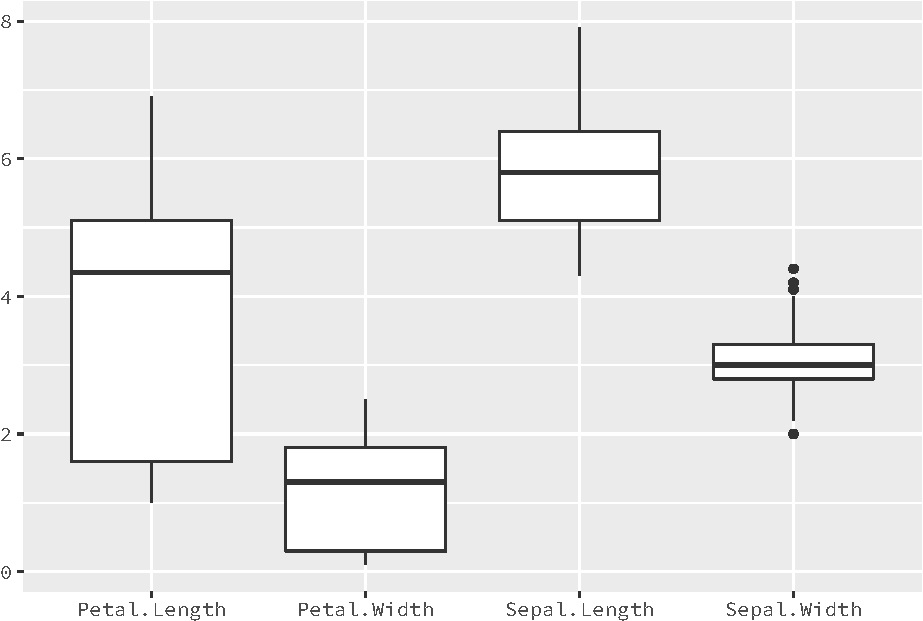
\includegraphics[width=0.9\linewidth,]{R_files/figure-latex/unnamed-chunk-4-1} 

}

\caption{花弁と萼片の分布}\label{fig:unnamed-chunk-4}
\end{figure}

 次に花弁(Petal)と萼片(Sepal)の幅と長さの関係を見てみます。

\begin{figure}[H]

{\centering \subfloat[花弁\label{fig:unnamed-chunk-5-1}]{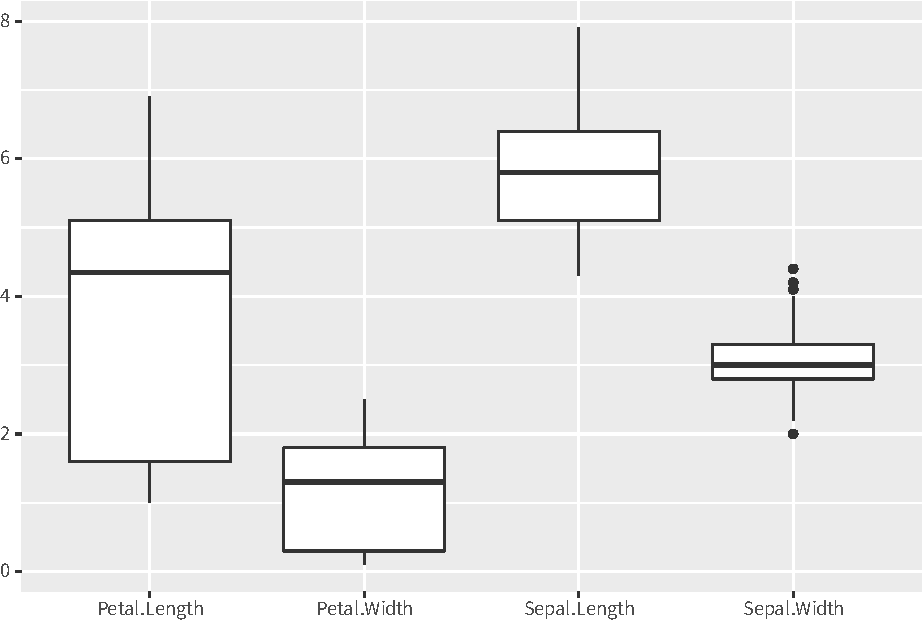
\includegraphics[width=0.4\linewidth,]{R_files/figure-latex/unnamed-chunk-5-1} }\subfloat[萼片\label{fig:unnamed-chunk-5-2}]{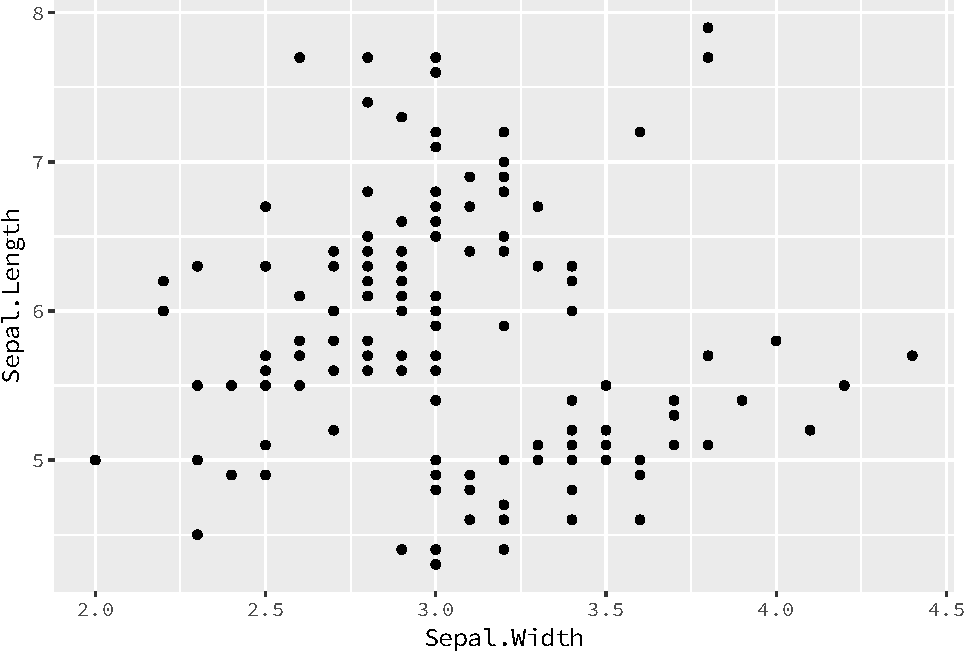
\includegraphics[width=0.4\linewidth,]{R_files/figure-latex/unnamed-chunk-5-2} }

}

\caption{幅と長さの関係}\label{fig:unnamed-chunk-5}
\end{figure}

 花弁(Petal)の幅と長さに相関関係があるように、萼片(Sepal)の方には相関関係がないように見えます。そこで、花弁(Petal)の幅(\texttt{Petal.Width})と長さ(\texttt{Petal.Length})の回帰式を求めます。

\begin{verbatim}
## 
## Call:
## lm(formula = Petal.Length ~ Petal.Width)
## 
## Residuals:
##      Min       1Q   Median       3Q      Max 
## -1.33542 -0.30347 -0.02955  0.25776  1.39453 
## 
## Coefficients:
##             Estimate Std. Error t value Pr(>|t|)    
## (Intercept)  1.08356    0.07297   14.85   <2e-16 ***
## Petal.Width  2.22994    0.05140   43.39   <2e-16 ***
## ---
## Signif. codes:  0 '***' 0.001 '**' 0.01 '*' 0.05 '.' 0.1 ' ' 1
## 
## Residual standard error: 0.4782 on 148 degrees of freedom
## Multiple R-squared:  0.9271, Adjusted R-squared:  0.9266 
## F-statistic:  1882 on 1 and 148 DF,  p-value: < 2.2e-16
\end{verbatim}

 回帰モデルの当てはまり具合がかなり良いので回帰モデルを可視化します。比較として萼片(Sepal)の回帰モデルも可視化します。

\begin{figure}[H]

{\centering \subfloat[花弁の回帰関係\label{fig:unnamed-chunk-7-1}]{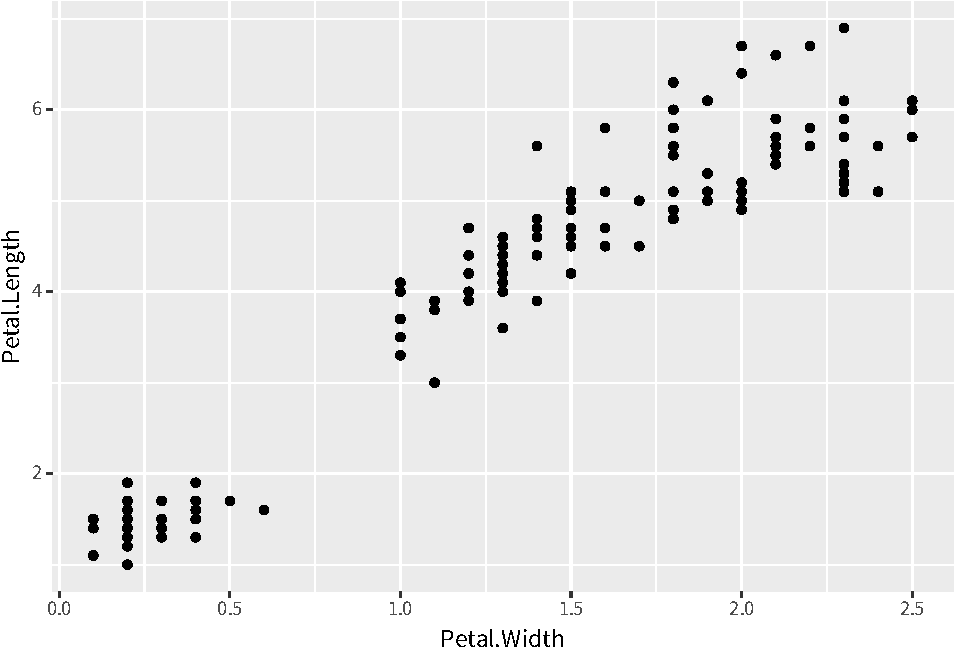
\includegraphics[width=0.4\linewidth,]{R_files/figure-latex/unnamed-chunk-7-1} }\subfloat[萼片の回帰関係\label{fig:unnamed-chunk-7-2}]{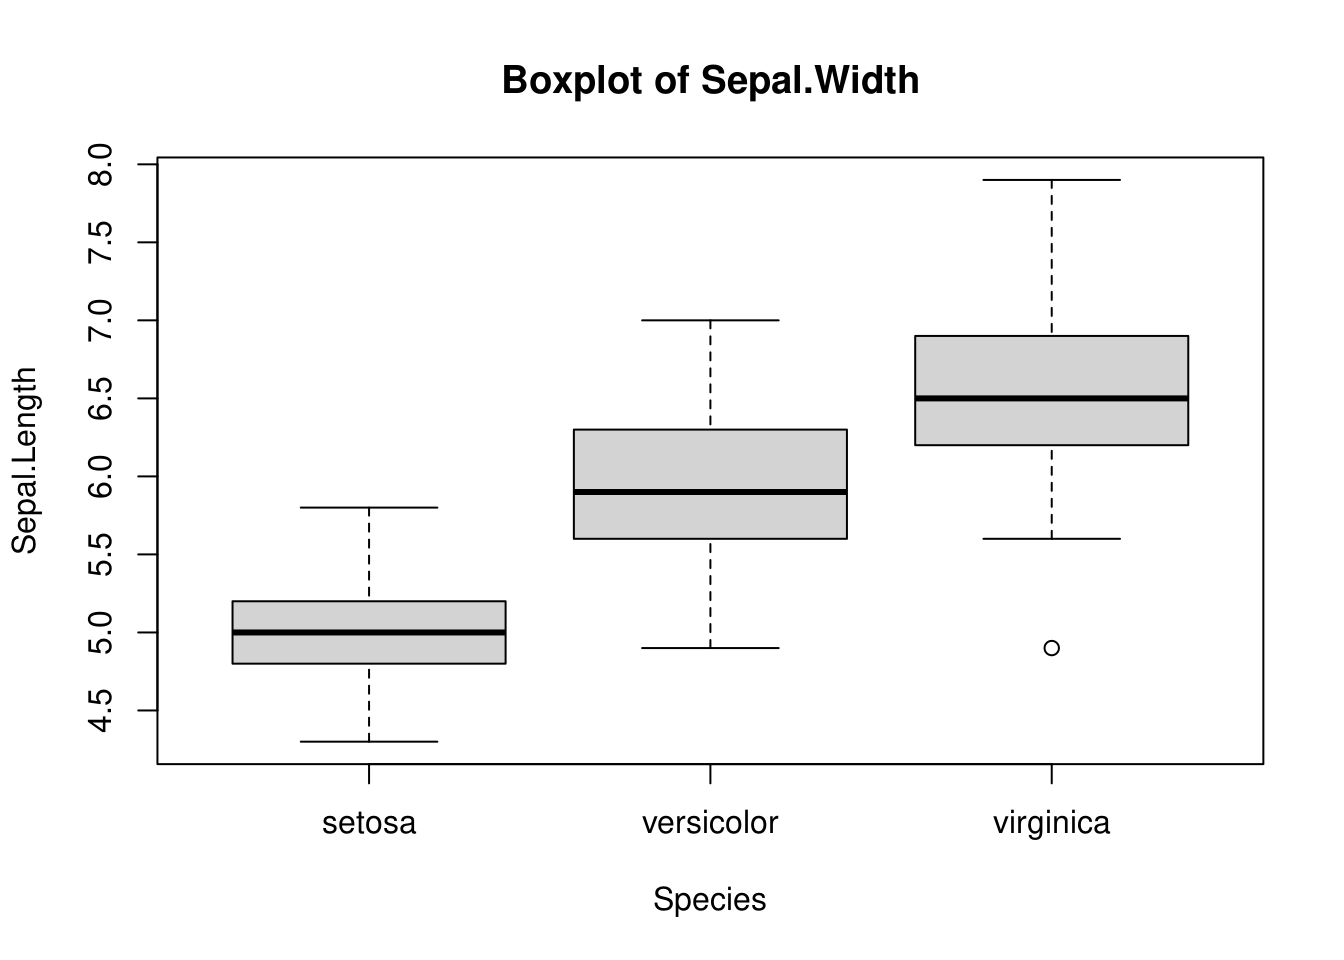
\includegraphics[width=0.4\linewidth,]{R_files/figure-latex/unnamed-chunk-7-2} }

}

\caption{幅と長さの関係}\label{fig:unnamed-chunk-7}
\end{figure}

 データ分析では、このような手順で対象のデータに対して可視化と変形、モデルの計算を繰り返すことで適切なモデルを探ります。これが基本となる分析プロセスです。

\begin{figure}[H]

{\centering 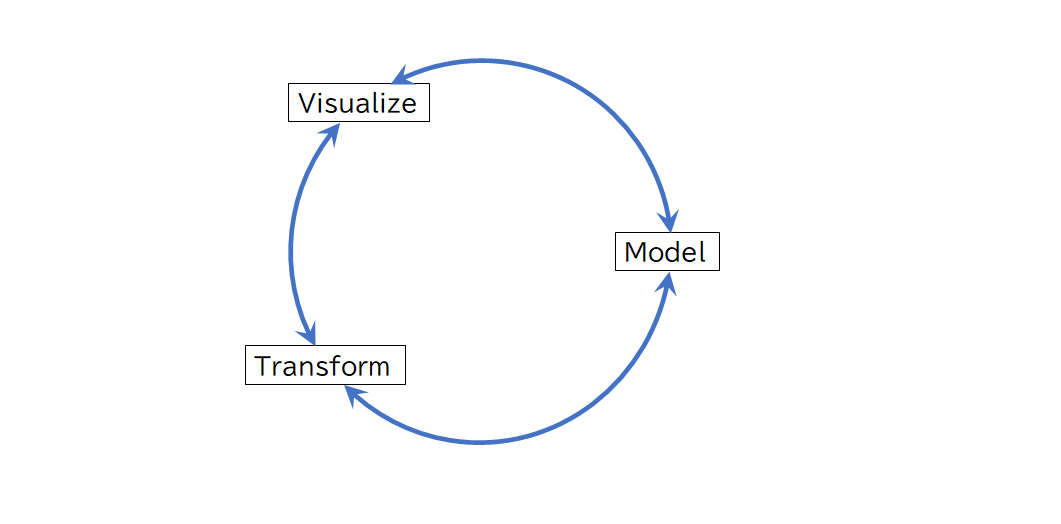
\includegraphics[width=0.9\linewidth,]{./fig/DSWF/data_science_workflow_step1} 

}

\caption{基本となる分析プロセス}\label{fig:unnamed-chunk-8}
\end{figure}

 実際には対象のデータが都合よく\textbf{R}に組み込まれている訳ではありませんので、対象となるデータを読み込み(インポート)、処理がしやすいように整形してから可視化などを行います。最後に分析結果を報告(レポート)しますので、分析プロセスは下図になります。

\begin{figure}[H]

{\centering 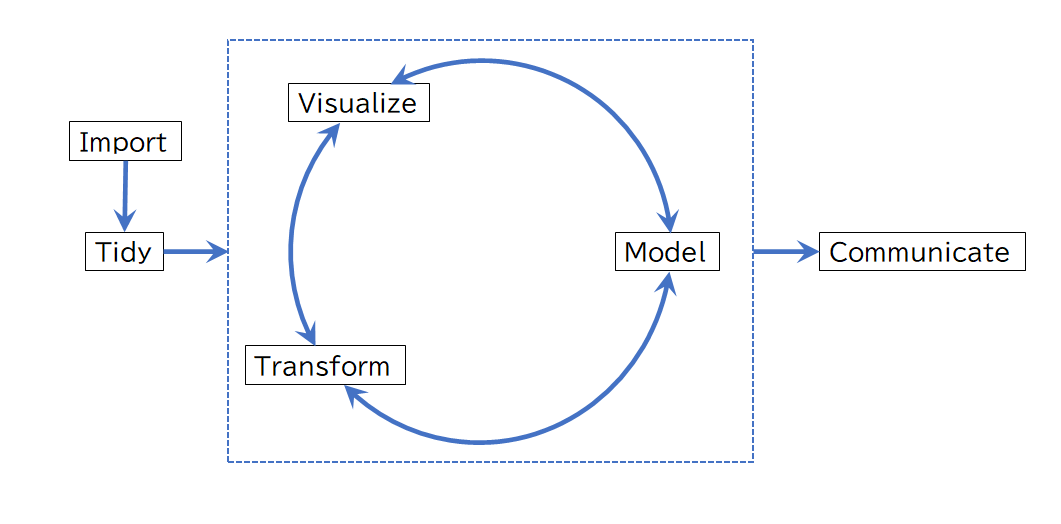
\includegraphics[width=0.9\linewidth,]{./fig/DSWF/data_science_workflow_step2} 

}

\caption{分析プロセス}\label{fig:unnamed-chunk-9}
\end{figure}

\hypertarget{data-science-workflow}{%
\section*{Data Science Workflow}\label{data-science-workflow}}
\addcontentsline{toc}{section}{Data Science Workflow}

実際には前節でのプロセスを\textbf{R}などのプログラム(プログラミング)でサポートすることによりプロセス全体を円滑に回せるよう仕組みも必要です。それを加えたものが「Data Science Workflow」と呼ばれるフロー図です。

\begin{figure}[H]

{\centering 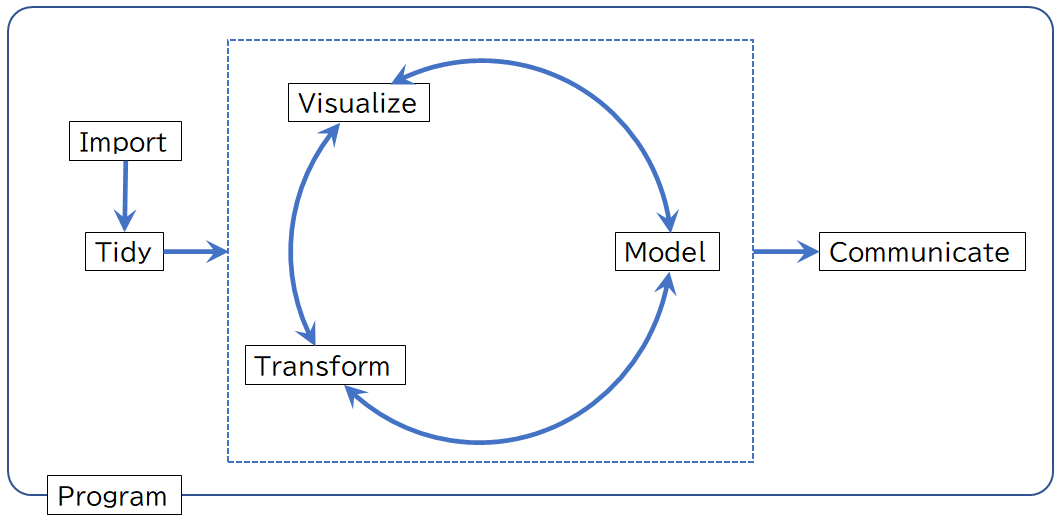
\includegraphics[width=0.9\linewidth,]{./fig/DSWF/data_science_workflow} 

}

\caption{Data Science Workflow}\label{fig:unnamed-chunk-10}
\end{figure}

「Data Science Workflow」自体は\textbf{R}コミュニティに多大な貢献をしている \href{http://hadley.nz/}{Hadley Wickham}が著書\href{https://r4ds.had.co.nz/}{『R for Data Science』}において提唱している概念です。

\begin{figure}[H]

{\centering 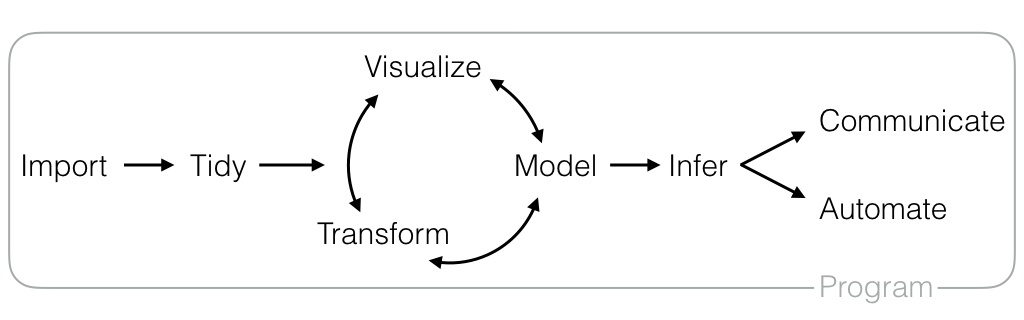
\includegraphics[width=0.9\linewidth,]{fig/data-science} 

}

\caption{Data Science Workflow, CC BY-NC-ND 3.0 US, Hadley Wickham}\label{fig:unnamed-chunk-11}
\end{figure}

Hadlyの図には前節の図にはない\textbf{Infer}と\textbf{Automate}すというプロセスが入っていますが、本書では\textbf{Infer}は\textbf{Model}に、\textbf{Automate}は\textbf{Communicate}に含まれるものとして考えています。

次章に移る前に個々のプロセスについて簡単な説明をしておきます。

\hypertarget{program}{%
\subsection*{Program}\label{program}}
\addcontentsline{toc}{subsection}{Program}

データ分析のすべてのプロセス(Import〜Communicate)で必要となるツールが\textbf{Program}です。\textbf{R}では様々なパッケージを使うことで外部アプリケーションとの連動を図り、\textbf{R}だけで全てのプロセスが完結するような「R Eco System」と呼べるような体型が出来上がりつつあります。この点は他のプログラミング言語と大きな違いです。

\hypertarget{import}{%
\subsection*{Import}\label{import}}
\addcontentsline{toc}{subsection}{Import}

分析対象となるデータを分析環境に取り込み分析をできるようにするのが\textbf{Import}プロセスです。データは様々な形式(文字コード、ファイル形式など)で保存されていますので、それらに見合った方法でインポートする必要があります。

\hypertarget{tidy}{%
\subsection*{Tidy}\label{tidy}}
\addcontentsline{toc}{subsection}{Tidy}

インポートしたデータは必ずしもデータ分析に適した形式になっているとは限りませんので、\textbf{R}で扱いやすいような形式(Tidy Data)にします。\href{https://www.jstatsoft.org/article/view/v059i10}{Tidy Data}\citep{R-TidyData}\index{Tidy Data}はデータ分析において非成に重要な概念で、以下の条件を満たしたデータを意味します。

\begin{itemize}
\tightlist
\item
  個々の変数が一つの列をなす
\item
  個々の観測が一つの行をなす
\item
  個々の観測の構成単位の累計が一つの表をなす
\item
  個々の値が一つのセルをなす
\end{itemize}

端的に表現すればデータの「構造と意味が合致する」と言えます。日本語では整然データと呼ばれることもあり、対義語は雑然データ(Messy Data)となります。

\hypertarget{transform}{%
\subsection*{Transform}\label{transform}}
\addcontentsline{toc}{subsection}{Transform}

整然データ(Tidy Data)に変換したとしても、データをそのまま状態で分析に使えることは稀です。実際のデータにはデータの一部が欠損していたり、分析には必要のないデータが含まれていたりしますので、不要なデータを削除したり(クレンジング)、必要なデータだけに絞り込んだり、新しい変数を計算したりする必要があります。これらの変換を事なうのが\textbf{Transform}プロセスです。

\textbf{Tidy}プロセスと合わせて\textbf{Wrangle}や\textbf{Data Wrangling}、前処理などと呼ばれることもあります。本書では\textbf{Import}、\textbf{Tidy}、\textbf{Transform}をあわせて\textbf{Wrangle}と称しています。

\hypertarget{visualize}{%
\subsection*{Visualize}\label{visualize}}
\addcontentsline{toc}{subsection}{Visualize}

文字通りデータの可視化を行うのが\textbf{Visualize}プロセスです。\textbf{R}には伝統的な\texttt{plot()}関数系を用いた可視化に加えて、\textbf{\texttt{ggplot2}}パッケージを用いた統一された文法による可視化があります。

\hypertarget{model}{%
\subsection*{Model}\label{model}}
\addcontentsline{toc}{subsection}{Model}

データを数式を用いてモデルにするのが\textbf{Model}プロセスです。本書では\textbf{Model}プロセスと\textbf{Infer}プロセスを合わせて\textbf{Model}プロセスと称しています。

\hypertarget{communicate}{%
\subsection*{Communicate}\label{communicate}}
\addcontentsline{toc}{subsection}{Communicate}

モデルが作成できましたら最後は分析結果を伝え(報告し)なければなりません。この報告のプロセスが\textbf{Communicate}で、プロセスにおいて重要な点が再現可能性(Reproducible research)です。再現可能性の重要性については\href{http://www.igaku-shoin.co.jp/paperDetail.do?id=PA03357_03}{「統計解析の再現可能性を高めるために」}をお読みください。

\hypertarget{tidyverse-ecosystem}{%
\section*{Tidyverse Ecosystem}\label{tidyverse-ecosystem}}
\addcontentsline{toc}{section}{Tidyverse Ecosystem}

Data Science Workflowを\textbf{R}で実現するための手段がHadley Wickhamが中心となって開発している\textbf{\texttt{tidyverse}}パッケージ群による「Tidyverse Ecosystem」です。

\begin{figure}[H]

{\centering 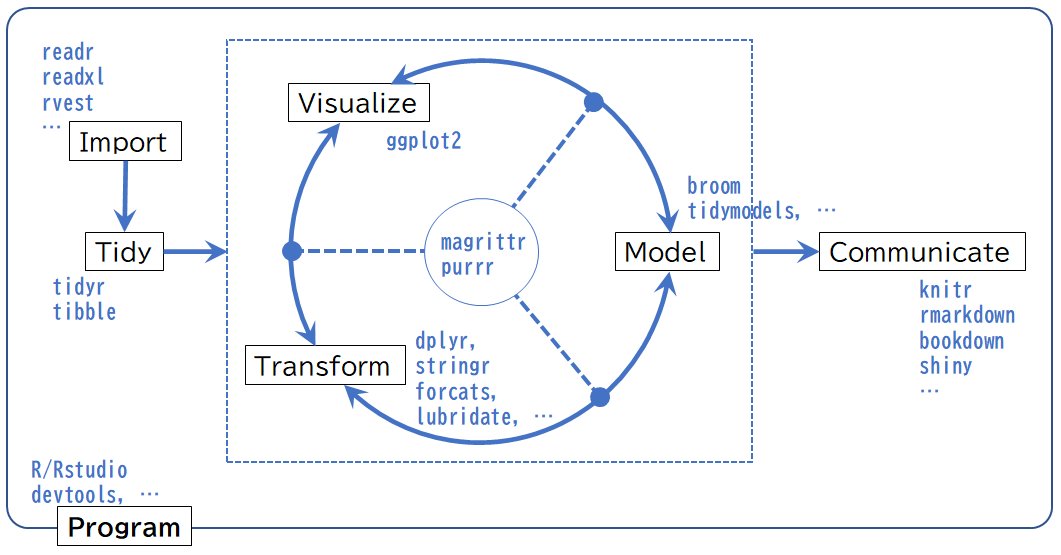
\includegraphics[width=0.9\linewidth,]{./fig/DSWF/tidyverse_eco_system} 

}

\caption{Tidyverse Ecosystem}\label{fig:unnamed-chunk-12}
\end{figure}

ここでは、主要なパッケージをいくつか紹介するに留めておきます。詳細は各分析プロセスの章、または、『RStartHere』\citep{RStartHere:GitHub}をご覧ください。

\begin{itemize}
\tightlist
\item
  \textbf{Import}

  \begin{itemize}
  \tightlist
  \item
    \textbf{\texttt{readr}} \citep{R-readr}

    \begin{itemize}
    \tightlist
    \item
      様々なテキスト形式テーブルを読み込むためのパッケージ
    \end{itemize}
  \item
    \textbf{\texttt{readxl}} \citep{R-readxl}

    \begin{itemize}
    \tightlist
    \item
      Microsoft Excelのファイルを読み込むためのパッケージ
    \end{itemize}
  \item
    \textbf{\texttt{rvest}} \citep{R-rvest}

    \begin{itemize}
    \tightlist
    \item
      Webスクレイピングのためのパッケージ
    \end{itemize}
  \item
    \textbf{\texttt{googlesheets4}} \citep{R-googlesheets4}

    \begin{itemize}
    \tightlist
    \item
      Google API v4 経由でスプレッドシートを読み込むためのパッケージ
    \end{itemize}
  \item
    \textbf{\texttt{DBI}} \citep{R-DBI}

    \begin{itemize}
    \tightlist
    \item
      SQL系の各種データベースと接続するためのパッケージ
    \end{itemize}
  \end{itemize}
\item
  \textbf{Tidy}

  \begin{itemize}
  \tightlist
  \item
    \textbf{\texttt{tidyr}} \citep{R-tidyr}

    \begin{itemize}
    \tightlist
    \item
      Tidy Dataの作成を強力にサポートしてくれるパッケージ
    \end{itemize}
  \item
    \textbf{\texttt{tibble}} \citep{R-tibble}

    \begin{itemize}
    \tightlist
    \item
      より厳密にTidy Dataを扱うためのパッケージ
    \end{itemize}
  \item
    \textbf{\texttt{zoo}} \citep{R-zoo}

    \begin{itemize}
    \tightlist
    \item
      時系列(TS)データを効率よく扱うためのパッケージ
    \end{itemize}
  \end{itemize}
\item
  \textbf{Visualize}

  \begin{itemize}
  \tightlist
  \item
    \textbf{\texttt{ggplot2}} \citep{R-ggplot2}

    \begin{itemize}
    \tightlist
    \item
      統一された文法で描画が行えるパッケージ
    \end{itemize}
  \item
    \textbf{\texttt{htmlwidgets}} \citep{R-htmlwidgets}

    \begin{itemize}
    \tightlist
    \item
      JavaScriptのウィジェットを利用できるパッケージ
    \end{itemize}
  \item
    \textbf{\texttt{patchwork}} \citep{R-patchwork}

    \begin{itemize}
    \tightlist
    \item
      \textbf{\texttt{ggplot2}}オブジェクトをひとつにまとめてレイアウトするためのパッケージ
    \end{itemize}
  \end{itemize}
\item
  \textbf{Transform}

  \begin{itemize}
  \tightlist
  \item
    \textbf{\texttt{dplyr}} \citep{R-dplyr}

    \begin{itemize}
    \tightlist
    \item
      Tidy Dataを様々な方法で操作するためのパッケージ
    \end{itemize}
  \item
    \textbf{\texttt{stringr}} \citep{R-stringr}

    \begin{itemize}
    \tightlist
    \item
      文字列処理をするためのパッケージ
    \end{itemize}
  \item
    \textbf{\texttt{forcats}} \citep{R-forcats}

    \begin{itemize}
    \tightlist
    \item
      因子型を操作するためのパッケージ
    \end{itemize}
  \item
    \textbf{\texttt{lubridate}} \citep{R-lubridate}

    \begin{itemize}
    \tightlist
    \item
      日付データを簡単に変換するためのパッケージ
    \end{itemize}
  \end{itemize}
\item
  \textbf{Model}

  \begin{itemize}
  \tightlist
  \item
    \textbf{\texttt{broom}} \citep{R-broom}

    \begin{itemize}
    \tightlist
    \item
      各種モデリング結果を整然データにするためのパッケージ
    \end{itemize}
  \item
    \textbf{\texttt{tidymodels}}\citep{tidymodels2020, R-tidymodels}

    \begin{itemize}
    \tightlist
    \item
      機械学習を中心としたモデリングフレームワーク
    \end{itemize}
  \end{itemize}
\item
  \textbf{Communicate}

  \begin{itemize}
  \tightlist
  \item
    \textbf{\texttt{knitr}} \citep{knitr2014, R-knitr}

    \begin{itemize}
    \tightlist
    \item
      \textbf{R}のコードと実行結果をPDFやHTMLなどに埋め込むためのパッケージ
    \end{itemize}
  \item
    \textbf{\texttt{rmarkdown}} \citep{R-rmarkdown}

    \begin{itemize}
    \tightlist
    \item
      マークダウン書式を用いてレポートを作成するためのパッケージ
    \end{itemize}
  \item
    \textbf{\texttt{bookdown}} \citep{bookdown2016, R-bookdown}

    \begin{itemize}
    \tightlist
    \item
      書籍や長いドキュメンを作成するためのパッケージ
    \end{itemize}
  \item
    \textbf{\texttt{shiny}} \citep{R-shiny}

    \begin{itemize}
    \tightlist
    \item
      インタラクティブなWebアプリケーションを作成するためのパッケージ
    \end{itemize}
  \end{itemize}
\item
  \textbf{Othres}

  \begin{itemize}
  \tightlist
  \item
    \textbf{\texttt{magrittr}} \citep{R-magrittr}

    \begin{itemize}
    \tightlist
    \item
      パイプ演算子(\texttt{\%\textgreater{}\%})によるスムースな処理を実現するパッケージ
    \end{itemize}
  \item
    \textbf{\texttt{purrr}} \citep{R-purrr}

    \begin{itemize}
    \tightlist
    \item
      関数型プログラミングによる反復処理を提供するパッケージ
    \end{itemize}
  \end{itemize}
\end{itemize}

 プロセスのハブ・スポークを担うパッケージもEcosystemの一部です。

\hypertarget{part-program}{%
\part{Program}\label{part-program}}

\hypertarget{ux5206ux6790ux74b0ux5883}{%
\chapter{分析環境}\label{ux5206ux6790ux74b0ux5883}}

\textbf{R}について学ぶ際には\textbf{R}が使えるような環境を用意しておくべきですが環境構築は初学者にとって最も厄介な作業です。そこで、初学者の方には環境構築の必要がない\textbf{Google Colab}の利用をおすゝめします。\textbf{RStudio}環境を構築できる方は、構築するのがベストです。

\hypertarget{ux4e3bux306aux5206ux6790ux74b0ux5883}{%
\section{主な分析環境}\label{ux4e3bux306aux5206ux6790ux74b0ux5883}}

\textbf{R}を利用した分析環境には以下のようなものがあります。

\begin{longtable}[]{@{}llccl@{}}
\caption{主な想定利用者と分析環境}\tabularnewline
\toprule
想定利用者 & 環境 & コード記述 & 再現可能性 & 備考 \\
\midrule
\endfirsthead
\toprule
想定利用者 & 環境 & コード記述 & 再現可能性 & 備考 \\
\midrule
\endhead
初学者 & R Commander & 不要 & 低 & 本書ではスコープ外 \\
初学者 & Exploratory & 不要 & 高 & 同上 \\
初学・中級者 & Google Colab & 要 & 高 & \\
中上級者 & RStudio Desktop & 要 & 高 & \\
中上級者 & RStudio Cloud & 要 & 高 & \\
中上級者 & RStudio Server & 要 & 高 & \\
開発者 & R + VS Code/Emacs & 要 & 高 & 本書ではスコープ外 \\
\bottomrule
\end{longtable}

\hypertarget{r-commander}{%
\subsection{R Commander}\label{r-commander}}

\href{https://socialsciences.mcmaster.ca/jfox/Misc/Rcmdr/}{R Commander(以降、\textbf{Rcmdr})}は、本書ではスコープ外ですが、\href{https://www.juse.or.jp/sqip/workshop/outline/index.html}{SQiP研究会の演習コース ソフトウエアメトリクス(以降、メトリクス演習コース)}におけるデフォルトツールですので簡単に紹介しておきます。 \textbf{Rcmdr}は\textbf{R}のパッケージとして提供されている GUIベースの対話型分析環境です。分析にあたって\textbf{R}のコードを記述する必要がありませんので、プログラミングの経験のない方でも利用することができます。ただし、実行できる機能(関数)が限定されている点と分析対象のデータの扱いに特有の考え方を用いてる点には注意が必要です。

\begin{figure}[H]

{\centering 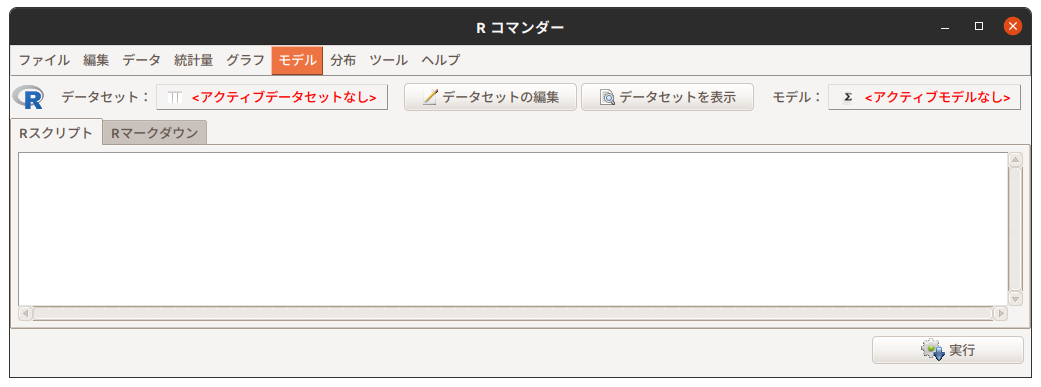
\includegraphics[width=0.9\linewidth,]{./fig/RCmdr} 

}

\caption{Rcmdr, Ubuntu}\label{fig:unnamed-chunk-13}
\end{figure}

\hypertarget{google-colab}{%
\subsection{Google Colab}\label{google-colab}}

\textbf{Google Colab}は Googleアカウントを持っていれば誰でも利用可能な\textbf{Python}向けの環境である\textbf{Jupyter Notebook}サービスです。\textbf{Jupyter Notebook}は\textbf{R}をエンジンとして利用することができますので、環境を構築することなく使い始めることができますので、初学者の演習環境としておすゝめです。

\begin{figure}[H]

{\centering 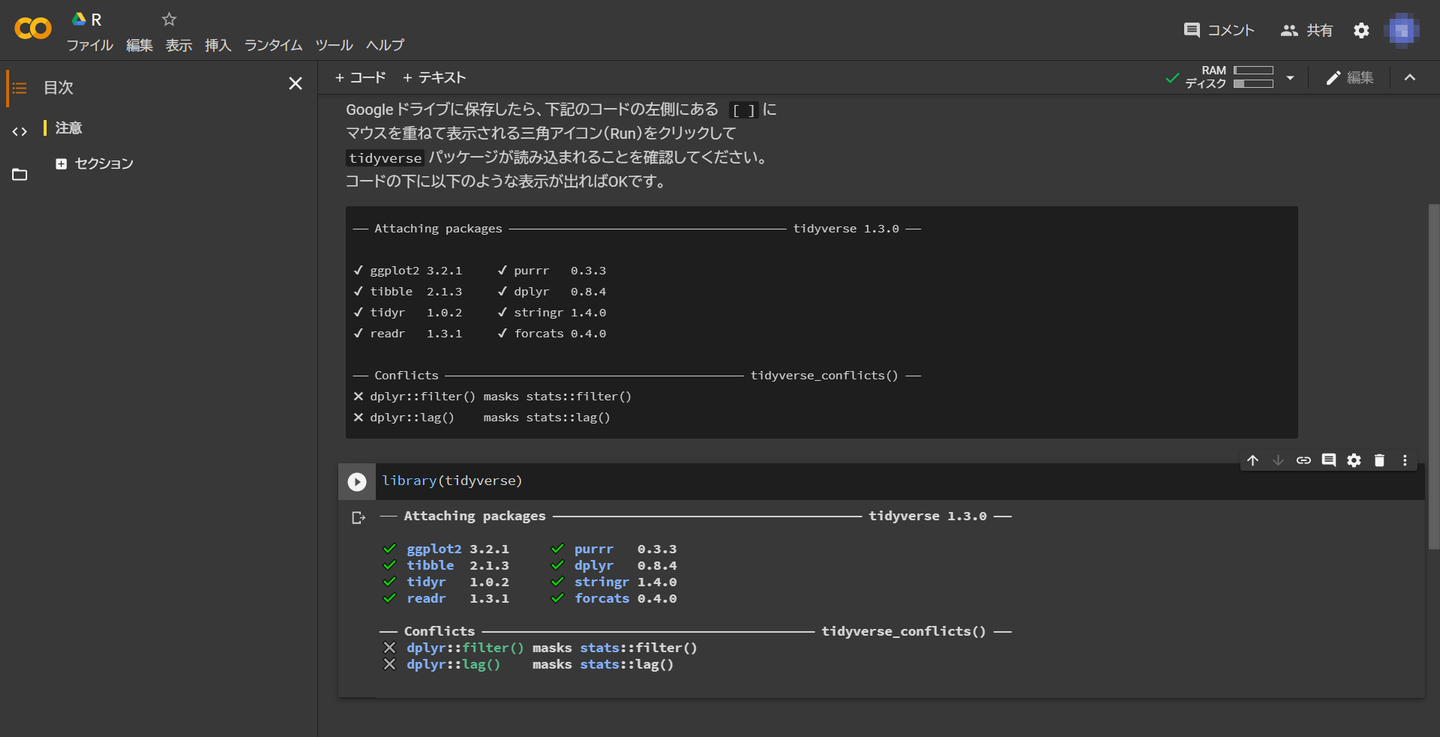
\includegraphics[width=0.9\linewidth,]{./fig/Colab/Firsttime} 

}

\caption{Google Colab}\label{fig:unnamed-chunk-14}
\end{figure}

\hypertarget{rstudio}{%
\subsection{RStudio}\label{rstudio}}

再現可能性を確保した探索的データ分析を行うのに最も適しているのが\textbf{RStudio}です。無償で使えるオープンソース版には、PC上のアプリケーションとして動作する\textbf{Desktop}と Webサーバとして動作する\textbf{Server}の二種類があります。 \textbf{RStudio}は\textbf{R}のデファクトスタンダード的な統合開発環境(IDE)であり、Tidyverse Eco Systemの中核とも言えます。その特徴として

\begin{itemize}
\tightlist
\item
  \textbf{R}のコードを記述するのに適したエディタを備えている
\item
  \textbf{R}のパッケージをインストール・管理するためのパッケージマネージャを備えている
\item
  \href{https://rmarkdown.rstudio.com/}{\textbf{R Markdown}}や \href{https://pandoc.org/}{\textbf{Pandoc}} との連携による再現可能性を確保するための仕組みを備えている
\item
  外部リソースからのデータを取り込む仕組み(\textbf{RStudio Connect})を備えている
\item
  複数の分析をプロジェクト単位で管理する仕組みを備えている
\item
  \href{https://git-scm.com/}{Git} などの外部プログラムと連携したソースの版管理の仕組みを備えている
\end{itemize}

などがあります。

\begin{figure}[H]

{\centering 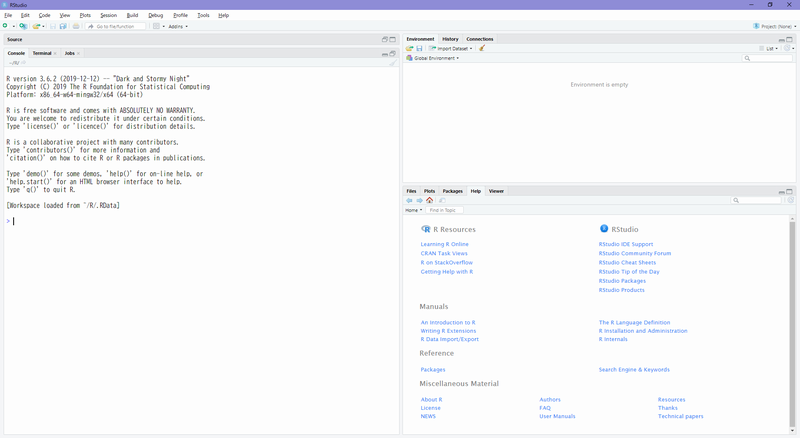
\includegraphics[width=0.9\linewidth,]{./fig/RStudio/DT} 

}

\caption{RStudio Desktop, Windows}\label{fig:unnamed-chunk-15}
\end{figure}

\textbf{RStudio Server}は\textbf{RStudio}をブラウザ経由で使う Linux 上で動作するサーバアプリケーションです。Dockerコンテナとして動作させることも可能ですので、個々の PC での分析環境を固定さたい場合には非常に便利です。

\begin{figure}[H]

{\centering 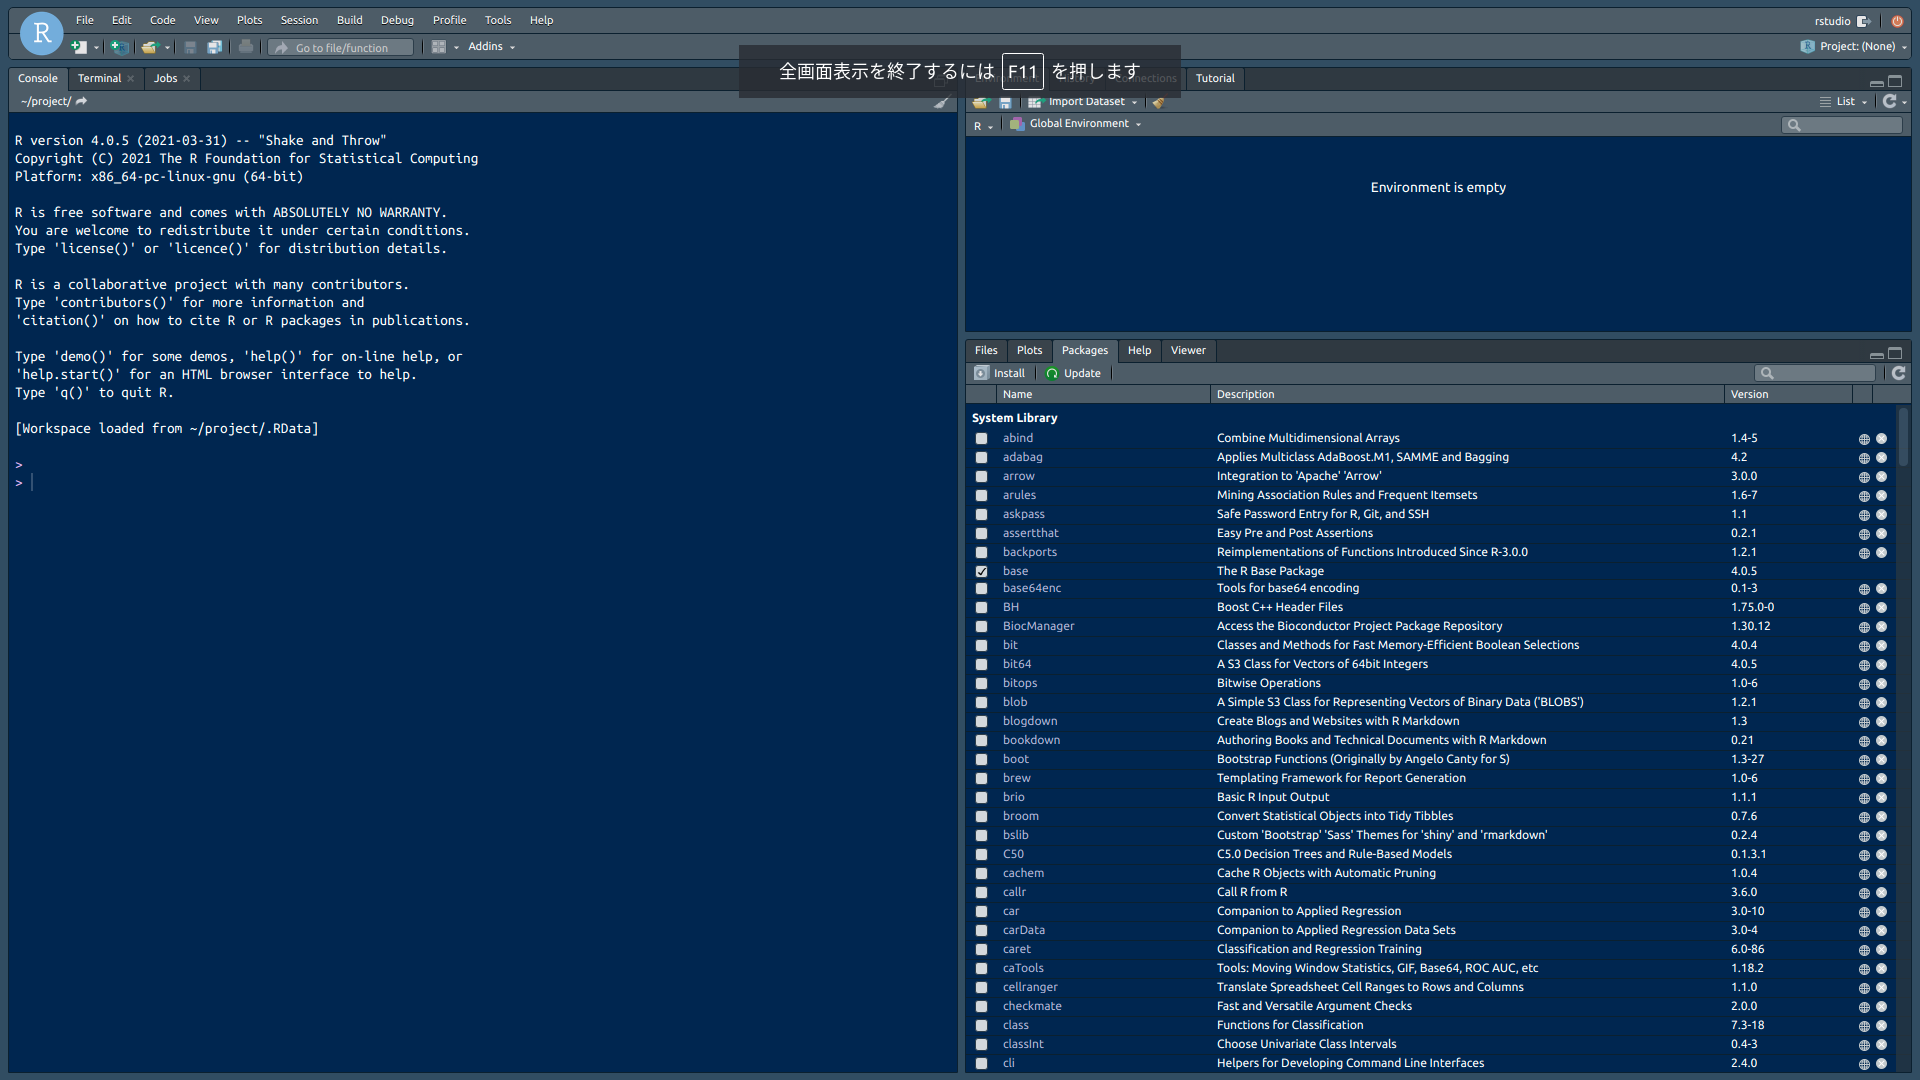
\includegraphics[width=0.9\linewidth,]{./fig/RStudio/RStudioServer} 

}

\caption{RStudio Server, Docker}\label{fig:unnamed-chunk-16}
\end{figure}

\hypertarget{rstudio-cloud}{%
\subsection{RStudio Cloud}\label{rstudio-cloud}}

\textbf{RStudio Cloud}は、その名の通りクラウド版の\textbf{RStudio}です。商用版の\textbf{RStudio Server Pro}をベースしていますので、任意のバージョンの\textbf{R}に切り替えて使うことや\textbf{RStduio Package Manager}とも連携しています。また、英語版ですがチュートリアル機能が充実しているのも特徴です。 無料プランが用意されていますが利用時間が15時間/月に限定されていますので、繋げっぱなしでの長時間利用には不向きです。

\begin{figure}[H]

{\centering 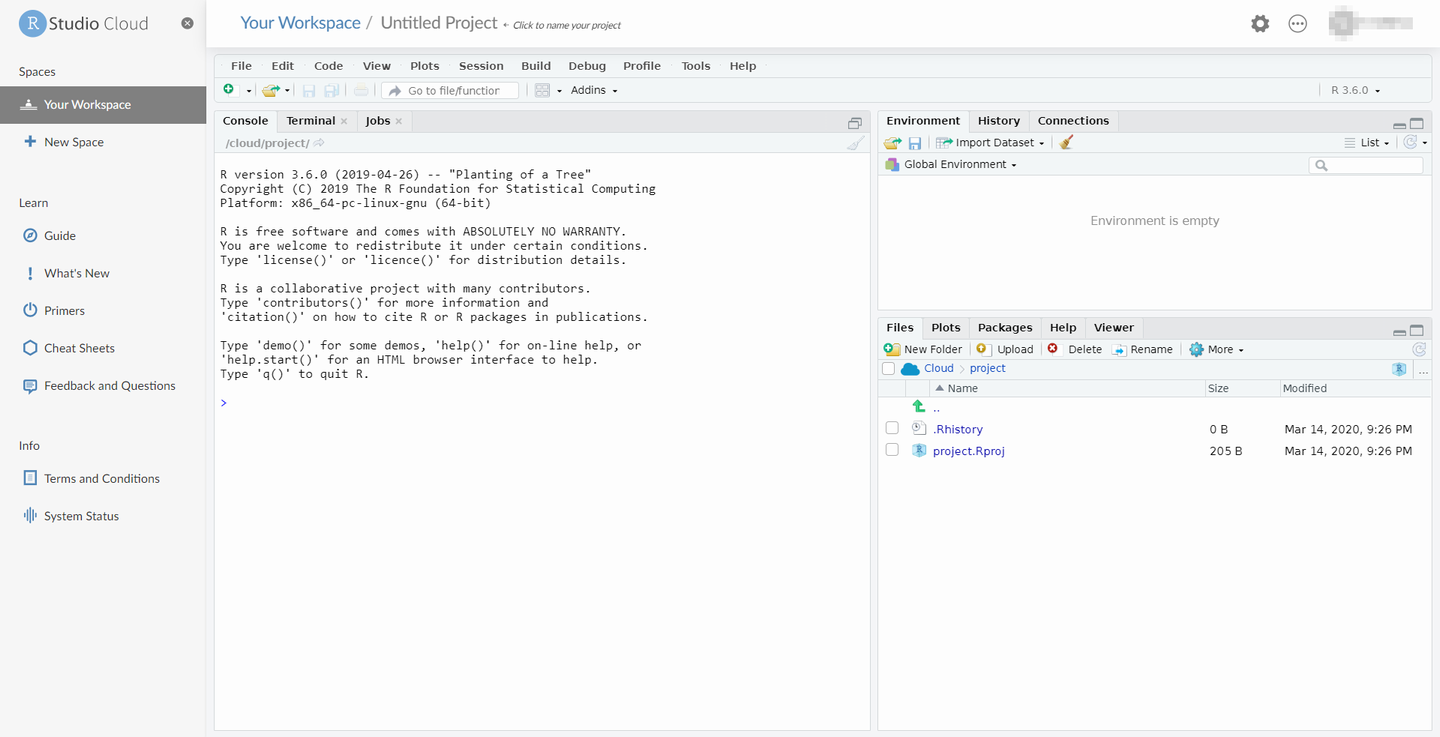
\includegraphics[width=0.9\linewidth,]{./fig/RStudio/RSCloud_01} 

}

\caption{RStudio Cloud}\label{fig:unnamed-chunk-17}
\end{figure}

\hypertarget{programing-editor}{%
\subsection{Programing Editor}\label{programing-editor}}

\textbf{R}の本体ははインタプリタ(対話的に逐次実行する処理系)として提供されていますので、\textbf{R}単体で動作させることが可能です。区別するために単体の\textbf{R}を\textbf{R Console}と呼ぶことがあります。 一部のプログラミングエディタでは機能拡張などを利用して直接\textbf{R Console}と連携してIDEのように\textbf{R}を利用することが可能です。古くはGNU Emacs用のESSや最近人気のあるMicrosoft VisualStudio Code用の機能拡張を使えば、お好みのエディタから直接\textbf{R}を使えるようになります。

\hypertarget{rux306eux57faux672c}{%
\chapter{Rの基本}\label{rux306eux57faux672c}}

\textbf{R}の文法説明が延々と続いてもつまらないので、本書では少し実用的な面から\textbf{R}のプログラミングを説明します。本チャプターでは『統計のはなし【改訂版】』\citep{ToukeinoHanashi}や『統計解析のはなし【改訂版】』\citep{ToukeiKaisekinoHanashi}を参考書として説明します。個々の詳細については、これらの書籍などを参照してください。 なお、基本文法については\protect\hyperlink{Appendix-RBasics}{Appendix R Basics}をご覧ください。

\hypertarget{ux5c3aux5ea6ux3068ux30c7ux30fcux30bfux578b}{%
\section{尺度とデータ型}\label{ux5c3aux5ea6ux3068ux30c7ux30fcux30bfux578b}}

分析対象となるデータは質的データと量的データに分類することができます。質的データは性別や品名、会社名など主に文字で表すことができる非数値データです。量的データは、温度や身長・体重、売上金額といった数値で表すことができるデータです。

\hypertarget{ux5c3aux5ea6ux6c34ux6e96}{%
\subsection{尺度水準}\label{ux5c3aux5ea6ux6c34ux6e96}}

質的データや量的データはデータ自体がもつ意味により下記のような尺度と呼ばれる水準で分類することができます。

\begin{itemize}
\tightlist
\item
  名義尺度

  \begin{itemize}
  \tightlist
  \item
    区別のためのラベルとしての意味を持つデータ
  \item
    同値か否かの比較しかできない
  \end{itemize}
\item
  順序尺度

  \begin{itemize}
  \tightlist
  \item
    区別のためのラベルとしての意味に加えて順番や大小関係の意味を持つデータ
  \item
    順番や大小の間隔には意味がない
  \item
    同値または大小比較の比較演算が可能
  \end{itemize}
\item
  間隔尺度

  \begin{itemize}
  \tightlist
  \item
    大小関係に加えて数値の差に意味をもつデータ
  \item
    数値の間隔には意味がありゼロは相対的な意味しかもたない
  \item
    比較演算に加えて加減算が可能
  \end{itemize}
\item
  比例尺度

  \begin{itemize}
  \tightlist
  \item
    大小関係、数値の差に加えて数値の比にも意味をもつデータ
  \item
    数値の間隔に意味がありゼロは原点としての(絶対的な)意味をもつ
  \item
    比較演算に加えて加減乗除が可能
  \item
    比尺度とも呼ばれる
  \end{itemize}
\end{itemize}

\begin{longtable}[]{@{}lll@{}}
\toprule
尺度水準 & 可能な演算 & データの例 \\
\midrule
\endhead
名義尺度 & 同値比較 & 名前、性別、背番号、血液型など \\
順序尺度 & 比較演算 & 着順、ランキング、段階評価など \\
間隔尺度 & 比較演算、加減算 & 温度、時刻、日付など \\
比例尺度 & 比較演算、加減乗除算 & 長さ、重さ、金額など \\
\bottomrule
\end{longtable}

\hypertarget{ux540dux7fa9ux5c3aux5ea6ux306eux30c7ux30fcux30bfux578b}{%
\subsubsection{名義尺度のデータ型}\label{ux540dux7fa9ux5c3aux5ea6ux306eux30c7ux30fcux30bfux578b}}

名義尺度を扱うには順序なし因子型(\texttt{factor})というデータ型を用いるのが便利です。因子型は文字でも数字でも扱えます。 ただ、因子型では水準の追加・削除操作が厄介ですので、文字型、数値型

\hypertarget{ux9806ux5e8fux5c3aux5ea6ux306eux30c7ux30fcux30bfux578b}{%
\subsubsection{順序尺度のデータ型}\label{ux9806ux5e8fux5c3aux5ea6ux306eux30c7ux30fcux30bfux578b}}

順序尺度は名義尺度のデータに順番や大小関係という属性を付与したデータと言えますので、順序付き因子型(\texttt{ordered})というデータ型を用いるのが便利です。

\hypertarget{ux9593ux9694ux5c3aux5ea6ux306eux30c7ux30fcux30bfux578b}{%
\subsubsection{間隔尺度のデータ型}\label{ux9593ux9694ux5c3aux5ea6ux306eux30c7ux30fcux30bfux578b}}

間隔尺度は数値のデータになりまので、データが取る値に合わせて、整数型(\texttt{integer})、実数型(\texttt{numeric})、日付型(\texttt{Date})のデータ型を用います。

\hypertarget{ux6bd4ux4f8bux5c3aux5ea6ux306eux30c7ux30fcux30bfux578b}{%
\subsubsection{比例尺度のデータ型}\label{ux6bd4ux4f8bux5c3aux5ea6ux306eux30c7ux30fcux30bfux578b}}

比例尺度は間隔尺度と同様に整数型(\texttt{integer})や実数型(\texttt{numeric})のデータ型を用います。

\hypertarget{ux8981ux7d04ux7d71ux8a08ux91cf}{%
\section{要約統計量}\label{ux8981ux7d04ux7d71ux8a08ux91cf}}

データを分析する前には分析対象となるデータがどのような特徴を持っているか確認しておくことが重要であるとよく言われます。この特徴を見るには要約統計量を使う場合が多いです。要約統計量はデータの分布の特徴を表すもので、記述統計量や基本統計量と呼ばれることもあります。

\hypertarget{ux5e73ux5747}{%
\subsection{平均}\label{ux5e73ux5747}}

算術平均(相加平均)は要約統計量の中でよく使われ、下式で求められます。

\begin{align}
  \bar{x} = \frac{x_1 + x_2 + \cdots + x_n}{n} = \frac{1}{n} \sum_{i = 1}^n x_i \label{eq:arithmetic-mean}
\end{align}

算術平均以外にも幾何平均(相乗平均)や \begin{align}
  \sqrt[n]{x_1 \times x_2 \times \cdots \times x_n} = \sqrt[n]{\prod_{i = 1}^n x_i} \label{eq:geometric-mean}
\end{align}

上記の他に値の下位・上位を任意の割合で除き平均(算術平均)を求めるトリム平均(刈込み平均・調整平均)という平均もあります。トリム平均は異常値や外れ値の影響を排除して平均を求めたい場合に利用されます。例えば体操競技で極端な点数を出す審査員の影響を排除するために使われます。この場合は全審査員の得点から最小と最大を除いたものから平均値を求め、その平均値を得点します。

平均といってもこのように様々な求め方がありますので、実際に\textbf{R}を使ってこれらの平均を求めてみます。

以降、灰色に網掛けされた部分が\textbf{R}のコード、コードの下の\texttt{\#\#}で始まる部分が実行結果(出力)になります。コードによっては実行結果が出力されない場合もあります。

\hypertarget{ux7b97ux8853ux5e73ux5747}{%
\subsubsection{算術平均}\label{ux7b97ux8853ux5e73ux5747}}

式\eqref{eq:arithmetic-mean}の算術平均は\texttt{mean()}関数で求めることができます。最初に平均の計算対象となるデータ(変数)を\texttt{c()}関数で作成します。\texttt{c()}関数はベクトル型の変数を作成する関数です。

\begin{Shaded}
\begin{Highlighting}[numbers=left,,]
\NormalTok{x }\OtherTok{\textless{}{-}} \FunctionTok{c}\NormalTok{(}\DecValTok{1}\NormalTok{, }\DecValTok{3}\NormalTok{, }\DecValTok{3}\NormalTok{, }\DecValTok{5}\NormalTok{, }\DecValTok{7}\NormalTok{)}
\end{Highlighting}
\end{Shaded}

\texttt{x}は値を代入(格納)する変数、\texttt{\textless{}-}は代入演算子\footnote{\textbf{R}では代入に\texttt{=}を使わないようにしてください}、\texttt{c()}関数はベクトルデータを作成する関数です。代入結果を確認するには以下を実行します。

\begin{Shaded}
\begin{Highlighting}[numbers=left,,]
\NormalTok{x}
\end{Highlighting}
\end{Shaded}

\begin{verbatim}
## [1] 1 3 3 5 7
\end{verbatim}

算出平均は\texttt{mean()}関数に計算対象となる\texttt{x}を指定して実行します。

\begin{Shaded}
\begin{Highlighting}[numbers=left,,]
\FunctionTok{mean}\NormalTok{(x)}
\end{Highlighting}
\end{Shaded}

\begin{verbatim}
## [1] 3.8
\end{verbatim}

\hypertarget{ux30c8ux30eaux30e0ux5e73ux5747}{%
\subsubsection{トリム平均}\label{ux30c8ux30eaux30e0ux5e73ux5747}}

トリム平均は算術平均のコードに引数\texttt{trim}を指定するだけです。引数\texttt{trim}は計算対象外にする割合を指定するオプションです。今回は五つのデータから最小値・最大値の二つを除いてトリム平均を求めますので\(\frac{2}{5} = 0.2\)を指定します。

\begin{Shaded}
\begin{Highlighting}[numbers=left,,]
\FunctionTok{mean}\NormalTok{(x, }\AttributeTok{trim =} \FloatTok{0.2}\NormalTok{)}
\end{Highlighting}
\end{Shaded}

\begin{verbatim}
## [1] 3.666667
\end{verbatim}

関数に指定できるオプションの引数を確認した場合場\texttt{?}に続いて関数名を\texttt{()}付きで打ち込んで実行してください。ヘルプが表示されます。

\begin{Shaded}
\begin{Highlighting}[numbers=left,,]
\NormalTok{?}\FunctionTok{mean}\NormalTok{()}
\end{Highlighting}
\end{Shaded}

\hypertarget{ux5e7eux4f55ux5e73ux5747}{%
\subsubsection{幾何平均}\label{ux5e7eux4f55ux5e73ux5747}}

式\eqref{eq:geometric-mean}の幾何平均(相乗平均)を求める関数は標準では用意されていません。パッケージを追加インストールする必要があります。ここでは\textbf{\texttt{psych}}パッケージを下記の手順でインストールして使います。なお、インストールに際してはインターネット接続が必要です。

\begin{enumerate}
\def\labelenumi{\arabic{enumi}.}
\tightlist
\item
  パッケージをインストールする
\item
  パッケージを読み込む
\end{enumerate}

パッケージのインストールは\texttt{install.packages()}関数を用います。\texttt{install.packages()}関数を実行すると環境によってはCRANミラーサイトの選択を促される場合があります。その場合は、最も近い地域のミラーサイトを選択してください。なお、パッケージのインストールは一度行えば次からのインストールは不要です。

\begin{Shaded}
\begin{Highlighting}[numbers=left,,]
\FunctionTok{install.packages}\NormalTok{(}\StringTok{"psych"}\NormalTok{)}
\end{Highlighting}
\end{Shaded}

インストールが完了しましたら\texttt{library()}関数を使ってパッケージを読み込みます。

\begin{Shaded}
\begin{Highlighting}[numbers=left,,]
\FunctionTok{library}\NormalTok{(psych)}
\end{Highlighting}
\end{Shaded}

使用している環境によっては他のパッケージの関数をマスクしているなどのメッセージが出力されますが、今は気にする必要ありません。

これで\textbf{\texttt{psych}}パッケージを使う準備が整いましたので、\texttt{geometric.mean()}関数で幾何平均を求めます。

\begin{Shaded}
\begin{Highlighting}[numbers=left,,]
\FunctionTok{geometric.mean}\NormalTok{(x)}
\end{Highlighting}
\end{Shaded}

\begin{verbatim}
## [1] 3.159818
\end{verbatim}

インストールしたパッケージの関数を使う場合、どのパッケージの関数を使っているかを明示的に示すために下記のように\texttt{::}演算子(名前空間へのアクセス演算子という)でパッケージ名と関数名をつなげて記述することもできます。

\begin{Shaded}
\begin{Highlighting}[numbers=left,,]
\NormalTok{psych}\SpecialCharTok{::}\FunctionTok{geometric.mean}\NormalTok{(x)}
\end{Highlighting}
\end{Shaded}

\begin{verbatim}
## [1] 3.159818
\end{verbatim}

この表記方法については賛否ありますが、どのパッケージの関数を使っているかが分かりやすいので本書ではこの記述方法を用います。

\hypertarget{ux9591ux8a71}{%
\subsubsection*{閑話}\label{ux9591ux8a71}}
\addcontentsline{toc}{subsubsection}{閑話}

\textbf{パッケージ四方山話}\\
 幾何平均を求めるために\texttt{psych}パッケージを利用しましたが、\textbf{R}には総積(\(x_1 \times x_2 \times \cdots \times x_n\))を求める\texttt{prod()}関数と累乗根(\(x^{\frac{1}{n}}\))を求めるべき乗演算子(\texttt{\^{}})がありますので、これを組み合わせれば幾何平均を求めることが可能です。

\begin{Shaded}
\begin{Highlighting}[numbers=left,,]
\FunctionTok{prod}\NormalTok{(x) }\SpecialCharTok{\^{}}\NormalTok{ (}\DecValTok{1} \SpecialCharTok{/} \FunctionTok{length}\NormalTok{(x))}
\end{Highlighting}
\end{Shaded}

\begin{verbatim}
## [1] 3.159818
\end{verbatim}

\texttt{length()}関数は変数\texttt{x}の長さ(変数\texttt{x}の中にある値の個数)を求める関数です。

幾何平均は全ての値を\texttt{prod()}関数で乗算しますのが、データの数が多い場合やデータの値が大きい(または、小さい)場合に\texttt{prod()}関数がオーバーフロー(または、アンダーフロー)を起こしてしまうことがあります。例えば、\(1\)から\(200\)までを乗算するとオーバーフローを起こします。

\begin{Shaded}
\begin{Highlighting}[numbers=left,,]
\FunctionTok{prod}\NormalTok{(}\FunctionTok{c}\NormalTok{(}\DecValTok{1}\SpecialCharTok{:}\DecValTok{200}\NormalTok{))}
\end{Highlighting}
\end{Shaded}

\begin{verbatim}
## [1] Inf
\end{verbatim}

一方、\texttt{geometric.mean()}関数は対策が施されていますのでオーバーフローを起こすことなく幾何平均を求めることができます。

\begin{Shaded}
\begin{Highlighting}[numbers=left,,]
\NormalTok{psych}\SpecialCharTok{::}\FunctionTok{geometric.mean}\NormalTok{(}\FunctionTok{c}\NormalTok{(}\DecValTok{1}\SpecialCharTok{:}\DecValTok{200}\NormalTok{))}
\end{Highlighting}
\end{Shaded}

\begin{verbatim}
## [1] 74.90045
\end{verbatim}

このように既にパッケージで提供されている関数があれば、自分でコードを組むよりはパッケージを導入した方が早くて確実です(ここでの本来の目的は幾何平均を求めることでなくデータの特徴を掴むことです)。特に\textbf{CRAN}に登録されているパッケージは審査が行われていますので、使わないよりは使った方が確実に目的を達成しやすくなります。\textbf{R}には先人の知恵が結集していますので、車輪の再発明に挑戦するより先人の知恵を活用する方をおすゝめします。

\hypertarget{ux5206ux6563ux6a19ux6e96ux504fux5dee}{%
\subsection{分散・標準偏差}\label{ux5206ux6563ux6a19ux6e96ux504fux5dee}}

データの散らばり具合を見るには分散・標準偏差がよく使われます。例えば、以下の\texttt{x}と\texttt{y}が取る値の範囲は同一ですが、同じ散らばり具合と言えるでしょうか?

\begin{Shaded}
\begin{Highlighting}[numbers=left,,]
\NormalTok{x }\OtherTok{\textless{}{-}} \FunctionTok{c}\NormalTok{(}\DecValTok{1}\NormalTok{, }\DecValTok{5}\NormalTok{, }\DecValTok{5}\NormalTok{, }\DecValTok{5}\NormalTok{, }\DecValTok{9}\NormalTok{)}
\FunctionTok{range}\NormalTok{(x)}
\end{Highlighting}
\end{Shaded}

\begin{verbatim}
## [1] 1 9
\end{verbatim}

\begin{Shaded}
\begin{Highlighting}[numbers=left,,]
\NormalTok{y }\OtherTok{\textless{}{-}} \FunctionTok{c}\NormalTok{(}\DecValTok{1}\NormalTok{, }\DecValTok{1}\NormalTok{, }\DecValTok{5}\NormalTok{, }\DecValTok{9}\NormalTok{, }\DecValTok{9}\NormalTok{)}
\FunctionTok{range}\NormalTok{(y)}
\end{Highlighting}
\end{Shaded}

\begin{verbatim}
## [1] 1 9
\end{verbatim}

散らばり具合を見るためにデータの個々の値と平均値との差の二乗の算術平均を分散(標本分散\(s^2\))、

\begin{align}
  s^2 = \frac{1}{n} \sum_{i = 1}^n (x_i - \bar{x})^2 \label{eq:variance}
\end{align}

単位を戻すために分散の平方根をとったものを標準偏差(標本標準偏差\(s\))と呼びます。

\begin{align}
  s = \sqrt{s^2} = \sqrt{\frac{1}{n} \sum_{i = 1}^n (x_i - \bar{x})^2} \label{eq:standatd-deviation}
\end{align}

しかし、\textbf{R}にはこの標本分散(\(s^2\))を求める関数は用意されていません。代わりに不偏分散(\(\hat{\sigma}^2\))を求める\texttt{var()}関数が用意されています。

\begin{align}
  \hat{\sigma}^2 &= \frac{1}{n - 1} \sum_{i = 1}^n (x_i - \bar{x})^2 \label{eq:var} \\
  &= var(x) \notag
\end{align}

式\eqref{eq:variance}\eqref{eq:var}から標本分散(\(s^2\))は\texttt{var()}関数を用いると

\begin{align}
  s^2 &= \frac{n - 1}{n}\hat{\sigma}^2 \label{eq:variance-var} \\
  &= \frac{length(x) - 1}{length(x)} \times var(x) \notag
\end{align}

のように求めることができます。標本標準偏差(\(s\))は式\eqref{eq:variance-var}の平方根を取ればいいこともわかります。

\hypertarget{ux30e2ux30fcux30e1ux30f3ux30c8}{%
\subsection{モーメント}\label{ux30e2ux30fcux30e1ux30f3ux30c8}}

本節の内容はデータ分析ではあまり使いませんので読み飛ばして頂いても結構です。

平均(分布の重心)と分散(分布の広がり)は、歪度(分布の左右非対称度合い)、尖度(分布の峰の尖り度合い)を含めて「モーメントから求められる要約統計量」と呼ぶことがあります。

\(n\)個のデータの平均値を

\begin{align}
  \bar{x} = \frac{1}{n}\sum_{i = 1}^{n}x_i \label{eq:moment1}
\end{align}

とした場合、平均値まわりの\(m\)次の中央モーメント\(\bar{x}_m\)を

\begin{align}
  \bar{x}_m = \frac{1}{n}\sum_{i = 1}^{n}(x_i - \bar{x})^m  (m = 2, 3, 4) \label{eq:moment}
\end{align}

と定義します。\(m = 2\)の場合、

\begin{align}
  \bar{x}_2 = \frac{1}{n}\sum_{i = 1}^{n}(x_i - \bar{x})^2 = s^2 \label{eq:moment2}
\end{align}

となりますので、\(\bar{x}_2\)は分散\(s^2\)であることがわかります。\(m = 3\)の場合、

\begin{align}
  \bar{x}_3 = \frac{1}{n}\sum_{i = 1}^{n}(x_i - \bar{x})^3 \label{eq:moment3}
\end{align}

となり、これを標準偏差の三乗(\(s^3\))で割ったもの

\begin{align}
  \gamma_1 = \frac{\bar{x}_3}{s^3} \label{eq:skewness}
\end{align}

を歪度(\(\gamma_1\))と呼びます。\(m = 4\)の場合、

\begin{align}
  \bar{x}_4 = \frac{1}{n}\sum_{i = 1}^{n}(x_i - \bar{x})^4  \label{eq:moment4}
\end{align}

となり、これを標準偏差の四乗、または、分散の二乗(\(s^4\))で割ったもの

\begin{align}
  \gamma_2 = \frac{\bar{x}_4}{s^4} \label{eq:kurtosise}
\end{align}

を尖度(\(\gamma_2\))と呼びます。

歪度や尖度を求める関数は標準では用意されていませんので\textbf{\texttt{e1071}}パッケージを用います。

\begin{Shaded}
\begin{Highlighting}[numbers=left,,]
\FunctionTok{install.packages}\NormalTok{(}\StringTok{"e1071"}\NormalTok{)}
\FunctionTok{library}\NormalTok{(e1071)}
\end{Highlighting}
\end{Shaded}

\hypertarget{ux6b6aux5ea6}{%
\subsubsection{歪度}\label{ux6b6aux5ea6}}

歪度はデータ分布の左右対象度合いです。左右対象となるデータ分布であれば\(0\)、右に歪んでいれば正の値を、左に歪んでいれば負の値を取ります。例えば下図のような分布では

\begin{figure}[H]

{\centering 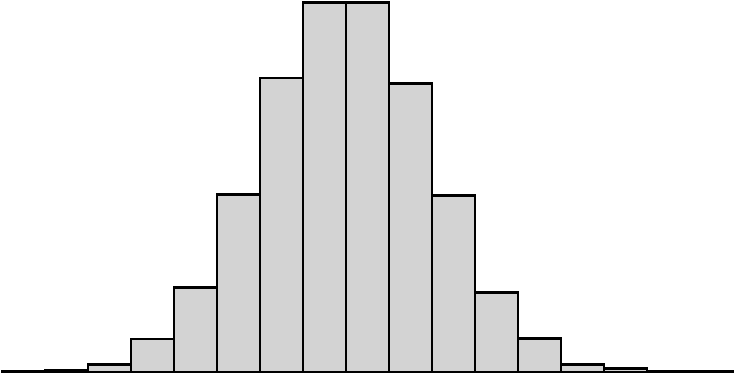
\includegraphics[width=0.9\linewidth,]{R_files/figure-latex/unnamed-chunk-32-1} 

}

\caption{正規分布に近い分布}\label{fig:unnamed-chunk-32}
\end{figure}

歪度はゼロに近い値となります。

\begin{Shaded}
\begin{Highlighting}[numbers=left,,]
\NormalTok{e1071}\SpecialCharTok{::}\FunctionTok{skewness}\NormalTok{(x)}
\end{Highlighting}
\end{Shaded}

\begin{verbatim}
## [1] 0.04548819
\end{verbatim}

次に下図のような分布では

\begin{figure}[H]

{\centering 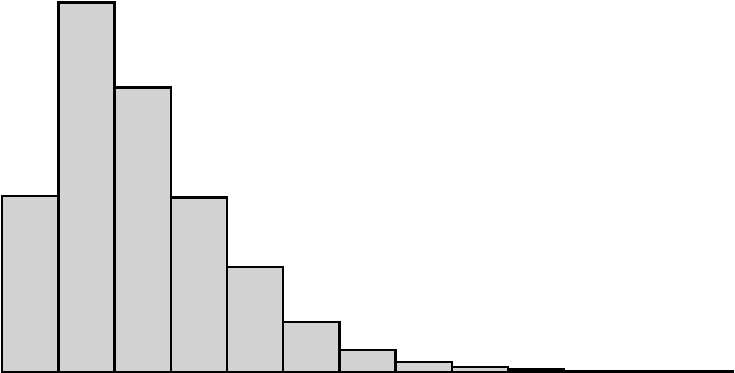
\includegraphics[width=0.9\linewidth,]{R_files/figure-latex/unnamed-chunk-34-1} 

}

\caption{右に歪んだ分布(左に偏った分布)}\label{fig:unnamed-chunk-34}
\end{figure}

歪度は正の値をとります。

\begin{Shaded}
\begin{Highlighting}[numbers=left,,]
\NormalTok{e1071}\SpecialCharTok{::}\FunctionTok{skewness}\NormalTok{(x)}
\end{Highlighting}
\end{Shaded}

\begin{verbatim}
## [1] 1.318739
\end{verbatim}

上図とは逆の分布では

\begin{figure}[H]

{\centering 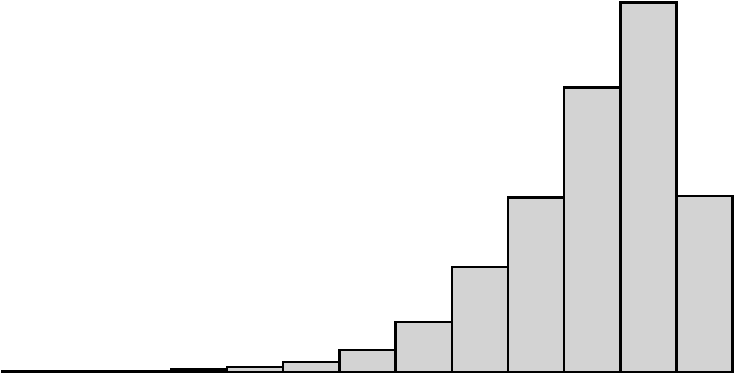
\includegraphics[width=0.9\linewidth,]{R_files/figure-latex/unnamed-chunk-36-1} 

}

\caption{左に歪んだ分布(右に偏った分布)}\label{fig:unnamed-chunk-36}
\end{figure}

歪度は負の値をとります。

\begin{Shaded}
\begin{Highlighting}[numbers=left,,]
\NormalTok{e1071}\SpecialCharTok{::}\FunctionTok{skewness}\NormalTok{(x)}
\end{Highlighting}
\end{Shaded}

\begin{verbatim}
## [1] -1.318739
\end{verbatim}

\hypertarget{ux5c16ux5ea6}{%
\subsubsection{尖度}\label{ux5c16ux5ea6}}

尖度はデータ分布の尖り具合です。標準正規分布と等しければ\(0\)、標準正規分布より尖ったt分布のような分布では正の値、広がった分布であれば負の値をとります。

\begin{figure}[H]

{\centering 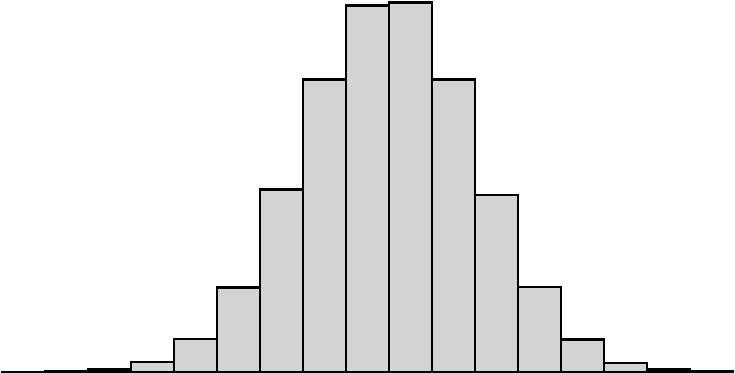
\includegraphics[width=0.9\linewidth,]{R_files/figure-latex/unnamed-chunk-38-1} 

}

\caption{正規分布に近い分布}\label{fig:unnamed-chunk-38}
\end{figure}

\begin{Shaded}
\begin{Highlighting}[numbers=left,,]
\NormalTok{e1071}\SpecialCharTok{::}\FunctionTok{kurtosis}\NormalTok{(x)}
\end{Highlighting}
\end{Shaded}

\begin{verbatim}
## [1] 0.01457407
\end{verbatim}

\begin{figure}[H]

{\centering 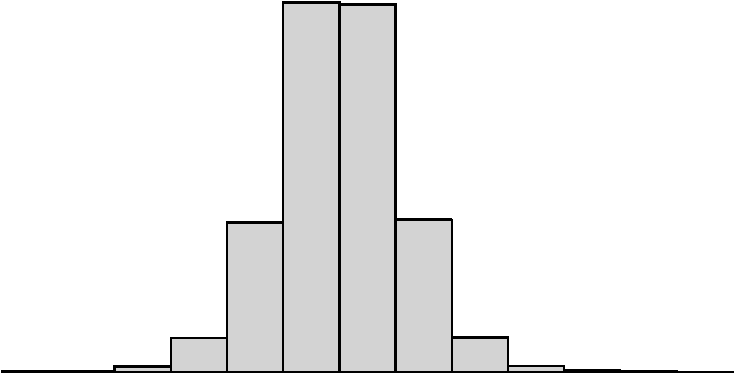
\includegraphics[width=0.9\linewidth,]{R_files/figure-latex/unnamed-chunk-40-1} 

}

\caption{中心部が高く幅の狭い尖った分布}\label{fig:unnamed-chunk-40}
\end{figure}

\begin{Shaded}
\begin{Highlighting}[numbers=left,,]
\NormalTok{e1071}\SpecialCharTok{::}\FunctionTok{kurtosis}\NormalTok{(x)}
\end{Highlighting}
\end{Shaded}

\begin{verbatim}
## [1] 0.7919764
\end{verbatim}

\begin{figure}[H]

{\centering 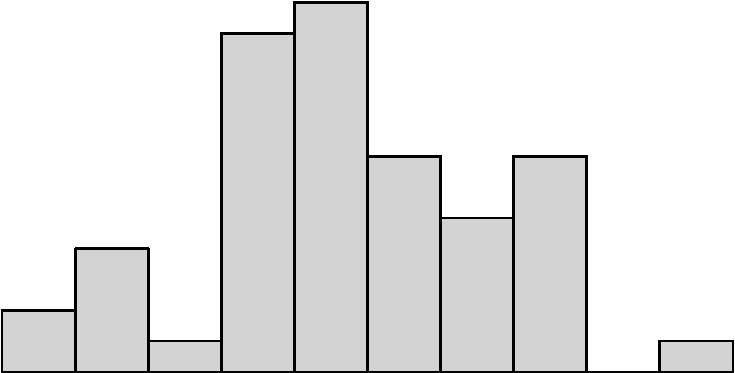
\includegraphics[width=0.9\linewidth,]{R_files/figure-latex/unnamed-chunk-42-1} 

}

\caption{中心部が低く横に広がった分布}\label{fig:unnamed-chunk-42}
\end{figure}

\begin{Shaded}
\begin{Highlighting}[numbers=left,,]
\NormalTok{e1071}\SpecialCharTok{::}\FunctionTok{kurtosis}\NormalTok{(x)}
\end{Highlighting}
\end{Shaded}

\begin{verbatim}
## [1] -0.3767132
\end{verbatim}

\hypertarget{ux4e2dux592eux5024}{%
\subsection{中央値}\label{ux4e2dux592eux5024}}

平均値や分散・標準偏差はデータの分布が平均値を中心に左右対象になっているような場合は有用な統計量ですが、データの分布が大きく歪んでいる対象に対しては適した統計量とは言えません。このような場合、平均値の代わりに中央値(中位数)や最頻値、分散・標準偏差に代わり範囲・分位範囲(分位値)を用いるます。これらの統計量はデータの中の位置を用いますので、データの分布に影響されることが少ないロバストネス(頑健性の高い)な統計量です。

中央値は文字通り中央(真ん中)に位置する値です。データを小さい順に並べて真ん中に位置する値で、\texttt{median()}関数を使って求めます。データが順番に並んでいなくても\texttt{median()}関数内でソート処理を行います。

\begin{Shaded}
\begin{Highlighting}[numbers=left,,]
\NormalTok{x }\OtherTok{\textless{}{-}} \FunctionTok{c}\NormalTok{(}\DecValTok{1}\NormalTok{, }\DecValTok{3}\NormalTok{, }\DecValTok{5}\NormalTok{, }\DecValTok{9}\NormalTok{, }\DecValTok{7}\NormalTok{)}
\FunctionTok{median}\NormalTok{(x)}
\end{Highlighting}
\end{Shaded}

\begin{verbatim}
## [1] 5
\end{verbatim}

データの長さ(値の数)が奇数の場合は、単純に中央の値(上記の場合は\(1, 3, 5, 7, 9\)なので中央に位置する\(5\))を返しますが、データの長さ偶数の場合は中央に近い両側の値の平均値(相加平均)を返します。

\begin{Shaded}
\begin{Highlighting}[numbers=left,,]
\NormalTok{x }\OtherTok{\textless{}{-}} \FunctionTok{c}\NormalTok{(}\DecValTok{1}\NormalTok{, }\DecValTok{3}\NormalTok{, }\DecValTok{5}\NormalTok{, }\DecValTok{9}\NormalTok{, }\DecValTok{7}\NormalTok{, }\DecValTok{6}\NormalTok{)}
\FunctionTok{median}\NormalTok{(x)}
\end{Highlighting}
\end{Shaded}

\begin{verbatim}
## [1] 5.5
\end{verbatim}

例えば、上記のようにデータの長さが偶数(\(6\))で\(1, 3, 5, 6, 7, 9\)というデータですので、中央に最も近い\(5, 6\)の平均値を中央値としています。

中央値と平均値を比較すると中央値がデータの分布に影響されにくい(ロバストネス)なことが分かります。

\begin{Shaded}
\begin{Highlighting}[numbers=left,,]
\NormalTok{x }\OtherTok{\textless{}{-}} \FunctionTok{c}\NormalTok{(}\DecValTok{1}\NormalTok{, }\DecValTok{3}\NormalTok{, }\DecValTok{5}\NormalTok{, }\DecValTok{9}\NormalTok{, }\DecValTok{7}\NormalTok{)}
\NormalTok{y }\OtherTok{\textless{}{-}} \FunctionTok{c}\NormalTok{(}\DecValTok{1}\NormalTok{, }\DecValTok{3}\NormalTok{, }\DecValTok{5}\NormalTok{, }\DecValTok{9}\NormalTok{, }\DecValTok{28}\NormalTok{)}
\end{Highlighting}
\end{Shaded}

\begin{Shaded}
\begin{Highlighting}[numbers=left,,]
\FunctionTok{median}\NormalTok{(x)                    }\CommentTok{\# 中央値の比較}
\end{Highlighting}
\end{Shaded}

\begin{verbatim}
## [1] 5
\end{verbatim}

\begin{Shaded}
\begin{Highlighting}[numbers=left,,]
\FunctionTok{median}\NormalTok{(y)                    }\CommentTok{\# 中央値の比較(大きい値には引っ張られない)}
\end{Highlighting}
\end{Shaded}

\begin{verbatim}
## [1] 5
\end{verbatim}

\begin{Shaded}
\begin{Highlighting}[numbers=left,,]
\FunctionTok{mean}\NormalTok{(x)                      }\CommentTok{\# 平均値の比較}
\end{Highlighting}
\end{Shaded}

\begin{verbatim}
## [1] 5
\end{verbatim}

\begin{Shaded}
\begin{Highlighting}[numbers=left,,]
\FunctionTok{mean}\NormalTok{(y)                      }\CommentTok{\# 平均値の比較(大きい値に引っ張られている)}
\end{Highlighting}
\end{Shaded}

\begin{verbatim}
## [1] 9.2
\end{verbatim}

\hypertarget{ux7bc4ux56f2}{%
\subsection{範囲}\label{ux7bc4ux56f2}}

前述の\texttt{x}と\texttt{y}は、中央値で見る限りと同じデータになってしまいます。この結論はいささか不合理ですので、データのばらつきを範囲(レンジ)で見てみます。範囲を求めるには、その名の通りの\texttt{range()}を用います。

\begin{Shaded}
\begin{Highlighting}[numbers=left,,]
\NormalTok{x}
\end{Highlighting}
\end{Shaded}

\begin{verbatim}
## [1] 1 3 5 9 7
\end{verbatim}

\begin{Shaded}
\begin{Highlighting}[numbers=left,,]
\FunctionTok{range}\NormalTok{(x)}
\end{Highlighting}
\end{Shaded}

\begin{verbatim}
## [1] 1 9
\end{verbatim}

\begin{Shaded}
\begin{Highlighting}[numbers=left,,]
\NormalTok{y}
\end{Highlighting}
\end{Shaded}

\begin{verbatim}
## [1]  1  3  5  9 28
\end{verbatim}

\begin{Shaded}
\begin{Highlighting}[numbers=left,,]
\FunctionTok{range}\NormalTok{(y)}
\end{Highlighting}
\end{Shaded}

\begin{verbatim}
## [1]  1 28
\end{verbatim}

範囲でみると\texttt{y}の方が\texttt{x}よりばらついていることが分かります。

\texttt{range()}関数は最小値と最大値を一度に取得しています。最小値は\texttt{min()}関数、最大値は\texttt{max()}関数で求められますので、\texttt{range()}関数は以下のように処理をしていることが分かります。

\begin{Shaded}
\begin{Highlighting}[numbers=left,,]
\FunctionTok{c}\NormalTok{(}\FunctionTok{min}\NormalTok{(x), }\FunctionTok{max}\NormalTok{(x))}
\end{Highlighting}
\end{Shaded}

\begin{verbatim}
## [1] 1 9
\end{verbatim}

最小値から最大値の幅を求めたい場合には\texttt{min()}関数と\texttt{max()}関数を用いるよりは\texttt{diff()}関数を用いた方が簡単です。

\begin{Shaded}
\begin{Highlighting}[numbers=left,,]
\FunctionTok{diff}\NormalTok{(}\FunctionTok{range}\NormalTok{(x))}
\end{Highlighting}
\end{Shaded}

\begin{verbatim}
## [1] 8
\end{verbatim}

\begin{Shaded}
\begin{Highlighting}[numbers=left,,]
\FunctionTok{diff}\NormalTok{(}\FunctionTok{range}\NormalTok{(y))}
\end{Highlighting}
\end{Shaded}

\begin{verbatim}
## [1] 27
\end{verbatim}

\hypertarget{ux56dbux5206ux4f4dux6570ux56dbux5206ux4f4dux7bc4ux56f2}{%
\subsection{四分位数・四分位範囲}\label{ux56dbux5206ux4f4dux6570ux56dbux5206ux4f4dux7bc4ux56f2}}

中央値は中位数と呼ばれるようにデータを二分の一にした場所にあるデータです。さらに細かくして全体を四分の一にしたの場所にあるデータを四分位数と呼びます。小さい方から見て最初の四分の一にある値を第一四分位数(\(25\%\)点、\(Q_1\))、次の四分の一にある値を第二四分位数(\(50\%\)点、\(Q_2\))、次の四分の一にある値を第三四分位数(\(75\%\)点、\(Q_3\))といいます。第二四分位数(\(50\%\)点、\(Q_2\))は中央値(中位数)とイコールです。 四分位数にも範囲があり、四分位範囲(\(IQR\), interquartile range)と呼ばれ以下のように定義されます、

\begin{align}
  IQR = Q_3 - Q_1 \label{eq:IQR}
\end{align}

四分位数は\texttt{quantile()}関数で求めることができます。オプションの引数を指定しなければ第一〜第三四分位数に加えて最小値(\(0\%点\))・最大値(\(100\%点\))を加えた五つの値が返ってきます。

\begin{Shaded}
\begin{Highlighting}[numbers=left,,]
\FunctionTok{quantile}\NormalTok{(x)}
\end{Highlighting}
\end{Shaded}

\begin{verbatim}
##   0%  25%  50%  75% 100% 
##    1    3    5    7    9
\end{verbatim}

任意の四分位数を求めたい場合は引数\texttt{prob}を指定します。\texttt{prob}は\(0\)〜\(1\)の間で指定する点に中位してください。

\begin{Shaded}
\begin{Highlighting}[numbers=left,,]
\FunctionTok{quantile}\NormalTok{(x, }\AttributeTok{prob =} \FloatTok{0.25}\NormalTok{)}
\end{Highlighting}
\end{Shaded}

\begin{verbatim}
## 25% 
##   3
\end{verbatim}

複数の四分位数を同時に求めことも可能です。

\begin{Shaded}
\begin{Highlighting}[numbers=left,,]
\FunctionTok{quantile}\NormalTok{(x, }\AttributeTok{prob =} \FunctionTok{c}\NormalTok{(}\FloatTok{0.25}\NormalTok{, }\FloatTok{0.75}\NormalTok{))}
\end{Highlighting}
\end{Shaded}

\begin{verbatim}
## 25% 75% 
##   3   7
\end{verbatim}

四分位範囲(\(IQR\))を求める場合は\texttt{IQR()}関数が便利です。

\begin{Shaded}
\begin{Highlighting}[numbers=left,,]
\FunctionTok{IQR}\NormalTok{(x)}
\end{Highlighting}
\end{Shaded}

\begin{verbatim}
## [1] 4
\end{verbatim}

\hypertarget{ux6700ux983bux5024}{%
\subsection{最頻値}\label{ux6700ux983bux5024}}

最頻値(モード)とは文字通り、最も頻繁に出てくる値のことです。例えば、以下の\texttt{x}と\texttt{y}は、平均値・中央値・範囲は全て同じ値になるデータです。

\begin{Shaded}
\begin{Highlighting}[numbers=left,,]
\NormalTok{x }\OtherTok{\textless{}{-}} \FunctionTok{c}\NormalTok{(}\DecValTok{1}\NormalTok{, }\DecValTok{1}\NormalTok{, }\DecValTok{3}\NormalTok{, }\DecValTok{5}\NormalTok{, }\DecValTok{9}\NormalTok{)}
\NormalTok{y }\OtherTok{\textless{}{-}} \FunctionTok{c}\NormalTok{(}\DecValTok{1}\NormalTok{, }\DecValTok{3}\NormalTok{, }\DecValTok{3}\NormalTok{, }\DecValTok{3}\NormalTok{, }\DecValTok{9}\NormalTok{)}
\FunctionTok{mean}\NormalTok{(x)}
\end{Highlighting}
\end{Shaded}

\begin{verbatim}
## [1] 3.8
\end{verbatim}

\begin{Shaded}
\begin{Highlighting}[numbers=left,,]
\FunctionTok{mean}\NormalTok{(y)}
\end{Highlighting}
\end{Shaded}

\begin{verbatim}
## [1] 3.8
\end{verbatim}

\begin{Shaded}
\begin{Highlighting}[numbers=left,,]
\FunctionTok{median}\NormalTok{(x)}
\end{Highlighting}
\end{Shaded}

\begin{verbatim}
## [1] 3
\end{verbatim}

\begin{Shaded}
\begin{Highlighting}[numbers=left,,]
\FunctionTok{median}\NormalTok{(y)}
\end{Highlighting}
\end{Shaded}

\begin{verbatim}
## [1] 3
\end{verbatim}

\begin{Shaded}
\begin{Highlighting}[numbers=left,,]
\FunctionTok{diff}\NormalTok{(}\FunctionTok{range}\NormalTok{(x))}
\end{Highlighting}
\end{Shaded}

\begin{verbatim}
## [1] 8
\end{verbatim}

\begin{Shaded}
\begin{Highlighting}[numbers=left,,]
\FunctionTok{diff}\NormalTok{(}\FunctionTok{range}\NormalTok{(y))}
\end{Highlighting}
\end{Shaded}

\begin{verbatim}
## [1] 8
\end{verbatim}

このようなデータに対しては最頻値を用いると平均値・中央値・範囲では見えなかった差異が見える場合があります。最頻値を求める関数は標準では用意されていませんので\texttt{modeest}パッケージを用います。

\begin{Shaded}
\begin{Highlighting}[numbers=left,,]
\FunctionTok{install.packages}\NormalTok{(}\StringTok{"modeest"}\NormalTok{)}
\FunctionTok{library}\NormalTok{(modeest)}
\end{Highlighting}
\end{Shaded}

\begin{Shaded}
\begin{Highlighting}[numbers=left,,]
\NormalTok{modeest}\SpecialCharTok{::}\FunctionTok{mfv}\NormalTok{(x)}
\end{Highlighting}
\end{Shaded}

\begin{verbatim}
## [1] 1
\end{verbatim}

\begin{Shaded}
\begin{Highlighting}[numbers=left,,]
\NormalTok{modeest}\SpecialCharTok{::}\FunctionTok{mfv}\NormalTok{(y)}
\end{Highlighting}
\end{Shaded}

\begin{verbatim}
## [1] 3
\end{verbatim}

\newpage

\hypertarget{ux307eux3068ux3081}{%
\subsection{まとめ}\label{ux307eux3068ux3081}}

本節に出てきた要約統計量と関数は下表の通りです。

\begin{longtable}[]{@{}lcl@{}}
\caption{要約統計量のまとめ}\tabularnewline
\toprule
要約統計量 & 表記 & \textbf{R}での求め方\footnote{引数\texttt{x}は計算対象となる数値データが格納されたベクトル型の変数} \\
\midrule
\endfirsthead
\toprule
要約統計量 & 表記 & \textbf{R}での求め方{} \\
\midrule
\endhead
標本平均 & \(\bar{x}\) & \texttt{mean(x)} \\
トリム平均 & & \texttt{mean(x,\ trim\ =\ t),\ t\ =\ 0\ to\ 0.5} \\
幾何平均 & & \texttt{psych::geometric.mean(x)} \\
標本分散 & \(s^2\) & \texttt{(length(x)\ -\ 1)\ /\ length(x)\ *\ var(x)} \\
不偏分散 & \(\hat{\sigma}^2\) & \texttt{var(x)} \\
標本標準偏差 & \(s\) & \texttt{sqrt((length(x)\ -\ 1)\ /\ length(x)\ *\ var(x))} \\
不偏標本偏差 & \(\hat{\sigma}\) & \texttt{sd(x)} \\
歪度 & \(\gamma_1\) & \texttt{e1071::skewness(x)} \\
尖度 & \(\gamma_2\) & \texttt{e1071::kurtosis(x)} \\
中央値 & & \texttt{median(x)} \\
範囲 & \(R\)\footnote{重相関計数を意味する場合もあり} & \texttt{range(x)} or \texttt{diff(range(x))} \\
四分位数 & \(Q_n\) & \texttt{quantile(x)} \\
第\(n\)四分位数 & \(Q_n\) & \texttt{quantile(x,\ probs\ =\ u),\ u\ =\ 0.25*n,\ n\ =\ 1,\ 2,\ 3}\footnote{引数\texttt{probs}はベクトル指定も可能(例:\texttt{probs\ =\ c(0.25,\ 0.75)})} \\
四分位範囲 & \(IQR\) & \texttt{IQR(x)} \\
最頻値 & & \texttt{modeest::mfv(x)} \\
\bottomrule
\end{longtable}

\newpage

\hypertarget{ux6f14ux7fd2}{%
\subsection{演習}\label{ux6f14ux7fd2}}

\hypertarget{ux6f14ux7fd2-1}{%
\subsubsection*{演習 1}\label{ux6f14ux7fd2-1}}
\addcontentsline{toc}{subsubsection}{演習 1}

標本分散(\(s^2\))と不偏分散(\(\hat{\sigma}^2\))の関係式\eqref{eq:variance-var}を用いて以下の二つのデータの標本分散(\(s^2\))を求めなさい。

\begin{Shaded}
\begin{Highlighting}[numbers=left,,]
\NormalTok{x }\OtherTok{\textless{}{-}} \FunctionTok{c}\NormalTok{(}\DecValTok{1}\NormalTok{, }\DecValTok{5}\NormalTok{, }\DecValTok{5}\NormalTok{, }\DecValTok{5}\NormalTok{, }\DecValTok{9}\NormalTok{)}
\NormalTok{y }\OtherTok{\textless{}{-}} \FunctionTok{c}\NormalTok{(}\DecValTok{1}\NormalTok{, }\DecValTok{1}\NormalTok{, }\DecValTok{5}\NormalTok{, }\DecValTok{9}\NormalTok{, }\DecValTok{9}\NormalTok{)}
\end{Highlighting}
\end{Shaded}

\hypertarget{ux6f14ux7fd2-2}{%
\subsubsection*{演習 2}\label{ux6f14ux7fd2-2}}
\addcontentsline{toc}{subsubsection}{演習 2}

欠損値を含む以下のデータの平均値(\(\bar{x}\))、不偏分散(\(\hat{\sigma}^2\))ならびに標本分散(\(s^2\))を求めなさい。

\begin{Shaded}
\begin{Highlighting}[numbers=left,,]
\NormalTok{z }\OtherTok{\textless{}{-}} \FunctionTok{c}\NormalTok{(}\DecValTok{1}\NormalTok{, }\DecValTok{5}\NormalTok{, }\ConstantTok{NA}\NormalTok{, }\DecValTok{7}\NormalTok{, }\DecValTok{9}\NormalTok{)}
\end{Highlighting}
\end{Shaded}

\begin{quote}
引数\texttt{na.rm}を指定します
\end{quote}

\hypertarget{ux6f14ux7fd2-3}{%
\subsubsection*{演習 3}\label{ux6f14ux7fd2-3}}
\addcontentsline{toc}{subsubsection}{演習 3}

\texttt{iris}データセットの各変量に対する四分位数を求めなさい。

\newpage

\hypertarget{ux30b3ux30e9ux30e0}{%
\subsection*{コラム}\label{ux30b3ux30e9ux30e0}}
\addcontentsline{toc}{subsection}{コラム}

\begin{rmdnote}
\textbf{英字?ギリシャ文字?}\\
 統計の書籍では様々な統計量を英字で表記する場合とギリシャ文字で表記する場合があり混乱しやすいのですが、英字(アルファベット)で表記されている場合は標本統計量、ギリシャ文字で表記されている場合は母集団の統計量もしくは母集団の推定統計量を意味しています。\\
 推定統計量を表記する場合、推定であることを意味するハット( \(\hat{}\) )という記号をつけます。平均と分散・標準偏差を使って整理すると下表のようになります。

\begin{longtable}[]{@{}lcccl@{}}
\caption{統計量の表記ルール}\tabularnewline
\toprule
統計量 & 平均 & 分散 & 標準偏差 & 備考 \\
\midrule
\endfirsthead
\toprule
統計量 & 平均 & 分散 & 標準偏差 & 備考 \\
\midrule
\endhead
母集団の統計量 & \(\mu\) & \(\sigma^2\) & \(\sigma\) & 神のみぞ知る統計量 \\
(不偏)推定量 & \(\hat{\mu}\) & \(\hat{\sigma}^2\) & \(\hat{\sigma}\) & 標本から母集団を推定した統計量 \\
標本統計量 & \(\bar{x}\) & \(s^2\) & \(s\) & 標本から求める統計量 \\
\bottomrule
\end{longtable}
 ハット( \(\hat{}\) )を省略している書籍や資料も散見されますので混乱しないように注意してください。詳しくは『統計的方法のしくみ』\citep{ToukeitekiHouhounoSikumi:jbook}の「3. 母数と統計量の区別」や『統計解析のはなし』\citep{ToukeiKaisekinoHanashi}の「2. 素人探偵物語」などを参照してください。 \end{rmdnote}

\newpage

\hypertarget{ux63a8ux5b9a}{%
\section{推定}\label{ux63a8ux5b9a}}

 前節で扱った要約統計量は与えられたデータに関する特徴を求めるもので、一般的には\textbf{記述統計}と呼ばれる手法に分類されます。一部、不偏推定量の記述がありますが、こちらは確率変数と確率分布の確率論をベースとした\textbf{推測統計}と呼ばれる手法に分類されます。推測統計は大きく統計的推定と統計的仮説検定に二分されます。本節では前者の統計的\textbf{推定}を扱います。

\hypertarget{ux6bcdux96c6ux56e3ux3068ux6a19ux672c}{%
\subsection{母集団と標本}\label{ux6bcdux96c6ux56e3ux3068ux6a19ux672c}}

 母集団とは分析の結果をもって説明したいデータの全体集合です。母集団の全てのデータを調べることができれば前述の記述統計の手法を適用することができますが、大抵の場合、母集団はとてつもなく大きな集団であったり、全数調査が困難\footnote{例えばテレビの世帯視聴率のように全世帯のデータを集めるとコスト的に見合わないような調査}だったりします。 そこで、標本と呼ばれる母集団から抽出した部分集合のデータが示す特徴を用いて母集団の特徴を推測することになります。しかしながら、標本のとり方よってはデータが偏ってしまい母集団の特徴からずれてしまう可能性がありす。そこで、確率論を用いて標本と母集団とのずれ(誤差の大きさ)を評価し信頼度つきで母集団の特徴を推測する推測統計の出番です。

\hypertarget{ux70b9ux63a8ux5b9a}{%
\subsection{点推定}\label{ux70b9ux63a8ux5b9a}}

 点推定は標本から求められる一つの推定値をもって母集団の特徴となる統計量の推定値とする方法です。例えば、前節で出てきた不偏分散は、まさにこの点推定の結果です。不偏推定値と言われることもあります。

母平均、母分散

\hypertarget{ux533aux9593ux63a8ux5b9a}{%
\subsection{区間推定}\label{ux533aux9593ux63a8ux5b9a}}

 一方、区間推定は文字通り幅を持たせて母集団の特徴となる統計量を推定する方法です。この幅を信頼区間(CI: Confidence Interval)と呼びます。

母平均、母比率、母分散

母平均の区間推定には大きく以下の二つの方法があります。

\begin{itemize}
\tightlist
\item
  母分散が既知の場合
\item
  母分散が未知の場合
\end{itemize}

通常は

\hypertarget{ux307eux3068ux3081-1}{%
\subsection{まとめ}\label{ux307eux3068ux3081-1}}

\hypertarget{ux6f14ux7fd2-4}{%
\subsection{演習}\label{ux6f14ux7fd2-4}}

\hypertarget{ux6f14ux7fd2-4-1}{%
\subsubsection*{演習 4}\label{ux6f14ux7fd2-4-1}}
\addcontentsline{toc}{subsubsection}{演習 4}

\hypertarget{ux6f14ux7fd2-5}{%
\subsubsection*{演習 5}\label{ux6f14ux7fd2-5}}
\addcontentsline{toc}{subsubsection}{演習 5}

\hypertarget{ux6f14ux7fd2-6}{%
\subsubsection*{演習 6}\label{ux6f14ux7fd2-6}}
\addcontentsline{toc}{subsubsection}{演習 6}

\hypertarget{ux691cux5b9a}{%
\section{検定}\label{ux691cux5b9a}}

データを分析する前には分析対象となるデータがどのような特徴を持っているか確認しておくことが重要であるとよく言われます。この特徴を見るには要約統計量を使う場合が多いです。要約統計量はデータの分布の特徴を表すもので、記述統計量や基本統計量と呼ばれることもあります。

\hypertarget{fux691cux5b9a}{%
\subsection{F検定}\label{fux691cux5b9a}}

\hypertarget{ux4e8cux9805ux691cux5b9a}{%
\subsection{二項検定}\label{ux4e8cux9805ux691cux5b9a}}

\hypertarget{ux307eux3068ux3081-2}{%
\subsection{まとめ}\label{ux307eux3068ux3081-2}}

\hypertarget{ux6f14ux7fd2-7}{%
\subsection{演習}\label{ux6f14ux7fd2-7}}

\hypertarget{ux6f14ux7fd2-7-1}{%
\subsubsection*{演習 7}\label{ux6f14ux7fd2-7-1}}
\addcontentsline{toc}{subsubsection}{演習 7}

\hypertarget{ux6f14ux7fd2-8}{%
\subsubsection*{演習 8}\label{ux6f14ux7fd2-8}}
\addcontentsline{toc}{subsubsection}{演習 8}

\hypertarget{ux6f14ux7fd2-9}{%
\subsubsection*{演習 9}\label{ux6f14ux7fd2-9}}
\addcontentsline{toc}{subsubsection}{演習 9}

\hypertarget{ux5206ux6563ux5206ux6790}{%
\section{分散分析}\label{ux5206ux6563ux5206ux6790}}

\hypertarget{ux307eux3068ux3081-3}{%
\subsection{まとめ}\label{ux307eux3068ux3081-3}}

\hypertarget{ux6f14ux7fd2-10}{%
\subsection{演習}\label{ux6f14ux7fd2-10}}

\hypertarget{ux6f14ux7fd2-10-1}{%
\subsubsection*{演習 10}\label{ux6f14ux7fd2-10-1}}
\addcontentsline{toc}{subsubsection}{演習 10}

\hypertarget{ux6f14ux7fd2-11}{%
\subsubsection*{演習 11}\label{ux6f14ux7fd2-11}}
\addcontentsline{toc}{subsubsection}{演習 11}

\hypertarget{ux6f14ux7fd2-12}{%
\subsubsection*{演習 12}\label{ux6f14ux7fd2-12}}
\addcontentsline{toc}{subsubsection}{演習 12}

\hypertarget{ux56deux5e30ux5206ux6790}{%
\section{回帰分析}\label{ux56deux5e30ux5206ux6790}}

\hypertarget{ux307eux3068ux3081-4}{%
\subsection{まとめ}\label{ux307eux3068ux3081-4}}

\hypertarget{ux6f14ux7fd2-13}{%
\subsection{演習}\label{ux6f14ux7fd2-13}}

\hypertarget{ux6f14ux7fd2-13-1}{%
\subsubsection*{演習 13}\label{ux6f14ux7fd2-13-1}}
\addcontentsline{toc}{subsubsection}{演習 13}

\hypertarget{ux6f14ux7fd2-14}{%
\subsubsection*{演習 14}\label{ux6f14ux7fd2-14}}
\addcontentsline{toc}{subsubsection}{演習 14}

\hypertarget{ux6f14ux7fd2-15}{%
\subsubsection*{演習 15}\label{ux6f14ux7fd2-15}}
\addcontentsline{toc}{subsubsection}{演習 15}

\hypertarget{part-wrangle}{%
\part{Wrangle}\label{part-wrangle}}

\hypertarget{import-1}{%
\chapter{Import}\label{import-1}}

 Import は

\begin{quote}
 Google Colab を利用する場合は[+コード]([Ctrl]+[M]+[Ctrl]+[B])ボタンでコードを追加してコードブロックを挿入してからコードを記載します。コードブロックの移動や削除はブロック右側に表示されているサブメニューで行います。[+テキスト]ボタンでテキストブロックを挿入すればコメントなどを書き込むことができます。
\end{quote}

 

\begin{quote}
 RStudio を利用する場合はメニューから[File]-[New File]-[R Notebook]を実行してR Notebook を作成します。キーボードショートカット[Ctrl/Cmd]+[Alt/Option]+[I]でコードチャンクを挿入しチャンクにコードを記述します。チャング以外にコメントなどを書き込むことができます。
\end{quote}

 

\hypertarget{readr}{%
\section{readr}\label{readr}}

\hypertarget{readxl}{%
\section{readxl}\label{readxl}}

\hypertarget{pdftools}{%
\section{pdftools}\label{pdftools}}

\hypertarget{tidy-1}{%
\chapter{Tidy}\label{tidy-1}}

\hypertarget{tidy-data}{%
\section{Tidy Data}\label{tidy-data}}

\hypertarget{longer}{%
\section{longer}\label{longer}}

\hypertarget{wider}{%
\section{wider}\label{wider}}

\hypertarget{transform-1}{%
\chapter{Transform}\label{transform-1}}

\hypertarget{filter}{%
\section{filter}\label{filter}}

\hypertarget{rename}{%
\section{rename}\label{rename}}

\hypertarget{select}{%
\section{select}\label{select}}

\hypertarget{select-helpers}{%
\subsection{select helpers}\label{select-helpers}}

\hypertarget{mutate}{%
\section{mutate}\label{mutate}}

\hypertarget{summarize}{%
\section{summarize}\label{summarize}}

\hypertarget{part-visualize}{%
\part{Visualize}\label{part-visualize}}

\hypertarget{base-r}{%
\chapter{Base R}\label{base-r}}

\hypertarget{plot}{%
\section{plot}\label{plot}}

\hypertarget{boxplot}{%
\section{boxplot}\label{boxplot}}

\hypertarget{hist}{%
\section{hist}\label{hist}}

\hypertarget{ggplot2}{%
\chapter{ggplot2}\label{ggplot2}}

\hypertarget{part-modelinfer}{%
\part{Model/Infer}\label{part-modelinfer}}

\hypertarget{test}{%
\chapter{Test}\label{test}}

\hypertarget{linear-model}{%
\chapter{Linear model}\label{linear-model}}

\hypertarget{machine-learning}{%
\chapter{Machine Learning}\label{machine-learning}}

\hypertarget{part-communicate}{%
\part{Communicate}\label{part-communicate}}

\hypertarget{r-markdown}{%
\chapter{R Markdown}\label{r-markdown}}

\hypertarget{part-automate}{%
\part{Automate}\label{part-automate}}

\hypertarget{shiny}{%
\chapter{shiny}\label{shiny}}

\hypertarget{part-appendix}{%
\part{APPENDIX}\label{part-appendix}}

\hypertarget{appendix-appendix}{%
\appendix \addcontentsline{toc}{chapter}{\appendixname}}


\hypertarget{references}{%
\chapter{References}\label{references}}

 文中で参照している文献・資料に関しては文献一覧のページを参照してください。なお、文献一覧はPDF版では巻末に「Bibliography」として、HTML版では参照ページの下部の「References」項にまとめてあります。

\begin{itemize}
\tightlist
\item
  RとRStudioのインストールと初期設定(PDF), 矢内 高知工科大学

  \begin{itemize}
  \tightlist
  \item
    \href{https://yukiyanai.github.io/jp/resources/docs/install-R_ubuntu.pdf}{Windows編}
  \item
    \href{https://yukiyanai.github.io/jp/resources/docs/install-R_macOS.pdf}{macOS編}
  \item
    \href{https://yukiyanai.github.io/jp/resources/docs/install-R_ubuntu.pdf}{Linux(Ubuntu)編}
  \end{itemize}
\item
  \href{https://www.soumu.go.jp/ict_skill/}{総務省 ICTスキル総合習得プログラム}

  \begin{itemize}
  \tightlist
  \item
    2017年度総務省「総務省 ICTスキル総合習得プログラム」事業の成果資料
  \end{itemize}
\item
  \href{https://github.com/tokyor/r-wakalang}{r-wakalang}

  \begin{itemize}
  \tightlist
  \item
    国内最大?のslackコミュニティ
  \end{itemize}
\end{itemize}

\hypertarget{Appendix-RBasics}{%
\chapter{R Basics}\label{Appendix-RBasics}}

\begin{quote}
Rの一番良いところは統計学者が作っているところだ。\\
Rの一番悪いところは統計学者が作っているところだ。
\end{quote}

\href{https://www.slideshare.net/shuyo/r-4022379}{出典}

\textbf{R}は統計的コンピューティングに特化している言語ですが、その開発は上記にもあるように統計学者が中心となって行われてきました。このような背景があるため他のコンピュータ言語を知っている方が使うと奇妙に感じる言語仕様があるかも知れません。 しかし、\textbf{R}の便利な点は統計的コンピューティングを行うに際して必須と言えるベクトル演算がデフォルトで使えることにあります。 まずは、このベクトル演算に慣れることから始めます。

コードの表記は以下のように灰色で網掛けされた部分が実行するコード、\texttt{\#\#} から始まる部分が実行結果となります。実行結果の表示がない場合は、次に実行するコードとあわせてコードが表示されます。なお、コード内の\texttt{\#}で始まる部分はコメントですので実行されません。

\begin{Shaded}
\begin{Highlighting}[numbers=left,,]
\NormalTok{x }\OtherTok{\textless{}{-}} \DecValTok{1}        \CommentTok{\# 変数への代入時は実行結果は表示されない}
\NormalTok{x             }\CommentTok{\# 表示させたい場合は、別途、変数のみで実行する}
\end{Highlighting}
\end{Shaded}

\begin{verbatim}
## [1] 1
\end{verbatim}

\begin{Shaded}
\begin{Highlighting}[numbers=left,,]
\FunctionTok{print}\NormalTok{(x)      }\CommentTok{\# もしくはprint()関数を用いる}
\end{Highlighting}
\end{Shaded}

\begin{verbatim}
## [1] 1
\end{verbatim}

実行結果の \texttt{\#\#} の後に表示されている \texttt{{[}{]}} 内の数値は実行結果の出力の数を示すためのインデックスです。実行環境の表示幅により表示される値が変わります。例えば 1 から 100 までの数字を表示した場合

\begin{verbatim}
##   [1]   1   2   3   4   5   6   7   8   9  10  11  12  13  14  15  16  17  18
##  [19]  19  20  21  22  23  24  25  26  27  28  29  30  31  32  33  34  35  36
##  [37]  37  38  39  40  41  42  43  44  45  46  47  48  49  50  51  52  53  54
##  [55]  55  56  57  58  59  60  61  62  63  64  65  66  67  68  69  70  71  72
##  [73]  73  74  75  76  77  78  79  80  81  82  83  84  85  86  87  88  89  90
##  [91]  91  92  93  94  95  96  97  98  99 100
\end{verbatim}

このように1行目は最初の値から表示されるので\texttt{{[}1{]}}に、2行目は1行目で18個表示されており19個目からの表示となるため\texttt{{[}19{]}}になっていることが分かります。

なお、以降に出てくるコードは\textbf{RStudio}上で動作するチュートリアルとしてパッケージ化してあります。興味のある方は \href{https://github.com/k-metrics/kmetrics}{パッケージ kmetrics} をインストールして使ってみてください。なお、パッケージ概要や動作環境はリンク先のページでご確認ください。

\hypertarget{ux57faux672cux7684ux306aux6f14ux7b97}{%
\section{基本的な演算}\label{ux57faux672cux7684ux306aux6f14ux7b97}}

最初に\textbf{R}の演算がどのような形式で行われるのかを紹介します。

\hypertarget{ux7b97ux8853ux6f14ux7b97}{%
\subsection{算術演算}\label{ux7b97ux8853ux6f14ux7b97}}

算術演算の基本である加減乗除算の四則演算は他のプログラミング言語や OS に付属の電卓アプリなどと同じです。

\begin{Shaded}
\begin{Highlighting}[numbers=left,,]
\DecValTok{1} \SpecialCharTok{+} \DecValTok{2}     \CommentTok{\# 加算}
\end{Highlighting}
\end{Shaded}

\begin{verbatim}
## [1] 3
\end{verbatim}

\begin{Shaded}
\begin{Highlighting}[numbers=left,,]
\DecValTok{2} \SpecialCharTok{{-}} \DecValTok{3}     \CommentTok{\# 減算}
\end{Highlighting}
\end{Shaded}

\begin{verbatim}
## [1] -1
\end{verbatim}

\begin{Shaded}
\begin{Highlighting}[numbers=left,,]
\DecValTok{3} \SpecialCharTok{*} \DecValTok{4}     \CommentTok{\# 乗算}
\end{Highlighting}
\end{Shaded}

\begin{verbatim}
## [1] 12
\end{verbatim}

\begin{Shaded}
\begin{Highlighting}[numbers=left,,]
\DecValTok{4} \SpecialCharTok{/} \DecValTok{5}     \CommentTok{\# 除算}
\end{Highlighting}
\end{Shaded}

\begin{verbatim}
## [1] 0.8
\end{verbatim}

\hypertarget{ux4ee3ux5165}{%
\subsection{代入}\label{ux4ee3ux5165}}

上記の演算結果を変数に代入してみます。代入には代入演算子(\texttt{\textless{}-})を用います。変数を使うための変数宣言は不要です。

\begin{Shaded}
\begin{Highlighting}[numbers=left,,]
\NormalTok{w }\OtherTok{\textless{}{-}} \DecValTok{1} \SpecialCharTok{+} \DecValTok{2}
\NormalTok{x }\OtherTok{\textless{}{-}} \DecValTok{2} \SpecialCharTok{*} \DecValTok{3}
\NormalTok{y }\OtherTok{\textless{}{-}} \DecValTok{3} \SpecialCharTok{{-}} \DecValTok{4}
\NormalTok{z }\OtherTok{\textless{}{-}} \DecValTok{4} \SpecialCharTok{/} \DecValTok{5}
\end{Highlighting}
\end{Shaded}

\hypertarget{ux4ee3ux5165ux7d50ux679cux306eux78baux8a8d}{%
\subsection{代入結果の確認}\label{ux4ee3ux5165ux7d50ux679cux306eux78baux8a8d}}

代入結果を確認するには変数名だけで実行するか \texttt{print()} 関数を用います。

\begin{Shaded}
\begin{Highlighting}[numbers=left,,]
\NormalTok{w}
\end{Highlighting}
\end{Shaded}

\begin{verbatim}
## [1] 3
\end{verbatim}

\begin{Shaded}
\begin{Highlighting}[numbers=left,,]
\NormalTok{x}
\end{Highlighting}
\end{Shaded}

\begin{verbatim}
## [1] 6
\end{verbatim}

\begin{Shaded}
\begin{Highlighting}[numbers=left,,]
\NormalTok{y}
\end{Highlighting}
\end{Shaded}

\begin{verbatim}
## [1] -1
\end{verbatim}

\begin{Shaded}
\begin{Highlighting}[numbers=left,,]
\NormalTok{z}
\end{Highlighting}
\end{Shaded}

\begin{verbatim}
## [1] 0.8
\end{verbatim}

\begin{Shaded}
\begin{Highlighting}[numbers=left,,]
\FunctionTok{print}\NormalTok{(w)}
\end{Highlighting}
\end{Shaded}

\begin{verbatim}
## [1] 3
\end{verbatim}

\begin{Shaded}
\begin{Highlighting}[numbers=left,,]
\FunctionTok{print}\NormalTok{(x)}
\end{Highlighting}
\end{Shaded}

\begin{verbatim}
## [1] 6
\end{verbatim}

\begin{Shaded}
\begin{Highlighting}[numbers=left,,]
\FunctionTok{print}\NormalTok{(y)}
\end{Highlighting}
\end{Shaded}

\begin{verbatim}
## [1] -1
\end{verbatim}

\begin{Shaded}
\begin{Highlighting}[numbers=left,,]
\FunctionTok{print}\NormalTok{(z)}
\end{Highlighting}
\end{Shaded}

\begin{verbatim}
## [1] 0.8
\end{verbatim}

\hypertarget{ux5408ux7b97}{%
\subsection{合算}\label{ux5408ux7b97}}

全ての変数を合算します。単純に加算演算子(\texttt{+})を用いても構いませんが、\texttt{sum()}という関数が用意されていますので、これを使います。

\begin{Shaded}
\begin{Highlighting}[numbers=left,,]
\FunctionTok{sum}\NormalTok{(w, x, y, z)    }\CommentTok{\# 3 + 6 + {-}1 + 0.8}
\end{Highlighting}
\end{Shaded}

\begin{verbatim}
## [1] 8.8
\end{verbatim}

\hypertarget{ux5e73ux5747-1}{%
\subsection{平均}\label{ux5e73ux5747-1}}

全ての変数の平均値を求めます。平均には

\begin{itemize}
\tightlist
\item
  算術平均(相加平均)
\item
  幾何平均(相乗平均)
\item
  トリム平均
\end{itemize}

がありますが、ここでは算術平均の値を求めます。算術平均の値を求めるには\texttt{mean()}という関数を用います。

\begin{Shaded}
\begin{Highlighting}[numbers=left,,]
\FunctionTok{mean}\NormalTok{(w, x, y, z)   }\CommentTok{\# (3 + 6 + {-}1 + 0.8) / 4}
\end{Highlighting}
\end{Shaded}

\begin{verbatim}
## [1] 3
\end{verbatim}

\texttt{sum()}関数と同じ指定をすると計算結果が期待と違います。これは\texttt{mean()}関数がとる引数が\texttt{sum()}関数と異なりひとつに限られるためです。そこで、ベクトル変数を作成する\texttt{c()}関数を用いて以下のように記述します。

\begin{Shaded}
\begin{Highlighting}[numbers=left,,]
\NormalTok{x }\OtherTok{\textless{}{-}} \FunctionTok{c}\NormalTok{(w, x, y, z)}
\FunctionTok{mean}\NormalTok{(x)}
\end{Highlighting}
\end{Shaded}

\begin{verbatim}
## [1] 2.2
\end{verbatim}

これで期待通りの値を得ることができました。

\hypertarget{ux5909ux6570ux306eux4e0aux66f8ux304d}{%
\subsection{変数の上書き}\label{ux5909ux6570ux306eux4e0aux66f8ux304d}}

さて、最初に\texttt{x}に代入した値は\texttt{6}でしたが、この時点では以下のように複数の値が代入されています。

\begin{Shaded}
\begin{Highlighting}[numbers=left,,]
\NormalTok{x}
\end{Highlighting}
\end{Shaded}

\begin{verbatim}
## [1]  3.0  6.0 -1.0  0.8
\end{verbatim}

これは平均値を求める際に\texttt{x}という変数を再利用したためですが、このように\textbf{R}では警告なしに既存の変数を上書きすることができます。注意してください。

このように\textbf{R}での演算は、他の言語と同様に何らかの値を変数に入れたり、何らかの値を関数で処理したりします。

\hypertarget{ux5909ux6570}{%
\section{変数}\label{ux5909ux6570}}

変数の命名規則は \href{https://style.tidyverse.org/syntax.html\#object-names}{tidyverse スタイルガイド(以降、スタイルガイド)} と呼ばれる記述ルールに準拠することをおすゝめします。スタイルガイドでは変数名に使える文字を以下の組合せであることを推奨しています。

\begin{itemize}
\tightlist
\item
  英数小文字(\texttt{A-Z}, \texttt{a-z})
\item
  数字(\texttt{0\ 1\ 2\ 3\ 4\ 5\ 6\ 7\ 8\ 9})
\item
  アンダースコア(\texttt{\_})
\end{itemize}

ただし、数字から始まる変数名は\textbf{R}の仕様により使うことができません(エラーになります)。また、日本語の変数名を使うことは可能ですが、様々な環境を考慮すると変数名に日本語を使用することはおすゝめできません。本書はスタイルガイドに準拠した記述になっています。

\hypertarget{ux4e88ux7d04ux8a9e}{%
\subsection{予約語}\label{ux4e88ux7d04ux8a9e}}

プログラミング言語には予約語(Reserved Word)といわれるものがあり予約語は変数名として使えません。\textbf{R}では以下が予約語になっています。

\texttt{if}, \texttt{else}, \texttt{for}, \texttt{while}, \texttt{repeat}, \texttt{in}, \texttt{next}, \texttt{break}, \texttt{function},\\
\texttt{TRUE}, \texttt{FALSE}, \texttt{NULL}, \texttt{NA}, \texttt{NaN}, \texttt{Inf}

また、予約語以外でも変数型や関数に使われている名前を変数名として使うことはおすゝめできません。

\hypertarget{ux30c7ux30fcux30bfux578b}{%
\subsection{データ型}\label{ux30c7ux30fcux30bfux578b}}

他の言語でも同じですが変数には値を入れることができます。データ型はどのような値のデータが入っているかを識別するためのものです。\textbf{R}の代表的なデータ型には以下のようなものがあります。

\begin{longtable}[]{@{}llllll@{}}
\toprule
型 & クラス & タイプ & モード & 格納モード & 備考 \\
\midrule
\endhead
実数型 & \texttt{numeric} & \texttt{double} & \texttt{numeric} & \texttt{double} & 倍精度浮動小数点 \\
整数型 & \texttt{integer} & \texttt{integer} & \texttt{numeric} & \texttt{integer} & \\
複素数型 & \texttt{complex} & \texttt{complex} & \texttt{complex} & \texttt{complex} & \\
論理型 & \texttt{logical} & \texttt{logical} & \texttt{logical} & \texttt{logical} & Boolean型 \\
文字型 & \texttt{character} & \texttt{character} & \texttt{character} & \texttt{character} & \\
日付型 & \texttt{Date} & \texttt{double} & \texttt{numeric} & \texttt{double} & Date型\textsuperscript{b} \\
\bottomrule
\end{longtable}

\textsuperscript{b} 日付型にはPOSIX型もあります

\textbf{R}は開発の経緯から様々な型の見かたがありますが、基本的に同じようなものだとと考えてください。書籍などでよく出てくる\texttt{str()}関数が返す型は上表におけるクラスです。

\hypertarget{ux5909ux6570ux578b}{%
\subsection{変数型}\label{ux5909ux6570ux578b}}

変数型はどのような形でデータを格納できるかを識別するためのものです。

\begin{longtable}[]{@{}lll@{}}
\toprule
変数型 & クラス & 説明 \\
\midrule
\endhead
ベクトル型 & データ型に同じ & 基本となる変数型 \\
因子型 & \texttt{factor}, \texttt{ordered} & インデックスを持つ変数型 \\
マトリクス型(行列型) & \texttt{matrix} & 二次元のベクトル型 \\
アレイ型(配列型) & \texttt{array} & 多次元のベクトル型 \\
データフレーム型 & \texttt{data.frame} & \textbf{等長}なベクトル型 \\
リスト型 & \texttt{list} & 自由度が最も高い変数型 \\
\bottomrule
\end{longtable}

\hypertarget{ux30d9ux30afux30c8ux30ebux578b}{%
\subsubsection{ベクトル型}\label{ux30d9ux30afux30c8ux30ebux578b}}

ベクトル型は基本となる変数型です。ベクトル型には一種類のデータ型のデータ(値)しか格納することができません。格納できる個数は任意です。 ベクトル型の変数を作成するには\texttt{c()}関数を用います。代入して\texttt{str()}関数でクラス、長さ(値の個数)と値を確認してみます。長さが1の場合は\texttt{c()}関数を省略することができます。

\begin{Shaded}
\begin{Highlighting}[numbers=left,,]
\NormalTok{x }\OtherTok{\textless{}{-}}\NormalTok{ 2L                 }\CommentTok{\# 一つだけ代入する場合 \textasciigrave{}c()\textasciigrave{} は省略可能}
\FunctionTok{str}\NormalTok{(x)                  }\CommentTok{\# 値が一つだけの場合は長さ表示が省略}
\end{Highlighting}
\end{Shaded}

\begin{verbatim}
##  int 2
\end{verbatim}

 

\begin{Shaded}
\begin{Highlighting}[numbers=left,,]
\NormalTok{x }\OtherTok{\textless{}{-}} \FunctionTok{c}\NormalTok{(}\DecValTok{1}\NormalTok{, }\DecValTok{2}\NormalTok{, }\DecValTok{3}\NormalTok{)         }\CommentTok{\# 実数の 1 から 3 の三つの値が代入}
\FunctionTok{str}\NormalTok{(x)                  }\CommentTok{\# []の部分が長さ表示}
\end{Highlighting}
\end{Shaded}

\begin{verbatim}
##  num [1:3] 1 2 3
\end{verbatim}

文字(型)を代入する場合はクォート(ダブルまはたシングル)で囲みます。

\begin{Shaded}
\begin{Highlighting}[numbers=left,,]
\NormalTok{x }\OtherTok{\textless{}{-}} \FunctionTok{c}\NormalTok{(}\StringTok{"1"}\NormalTok{, }\StringTok{\textquotesingle{}2\textquotesingle{}}\NormalTok{, }\StringTok{"3"}\NormalTok{)   }\CommentTok{\# 文字として数字を代入}
\FunctionTok{str}\NormalTok{(x)}
\end{Highlighting}
\end{Shaded}

\begin{verbatim}
##  chr [1:3] "1" "2" "3"
\end{verbatim}

では文字(型)と数字(型)を混在させたらどうなるでしょう?

\begin{Shaded}
\begin{Highlighting}[numbers=left,,]
\NormalTok{x }\OtherTok{\textless{}{-}} \FunctionTok{c}\NormalTok{(1L, }\DecValTok{2}\NormalTok{, }\StringTok{"3"}\NormalTok{)      }\CommentTok{\# 整数、実数、文字としての数字を代入}
\FunctionTok{str}\NormalTok{(x)                  }\CommentTok{\# 強制型変換により最も柔軟度の高い文字型に}
\end{Highlighting}
\end{Shaded}

\begin{verbatim}
##  chr [1:3] "1" "2" "3"
\end{verbatim}

エラーにはならずベクトル型変数は文字型の変数として作成されます。これは強制型変換という処理が行われるためです。強制型変換は複数のデータ型が混在した場合により柔軟度の高いデータ型に自動的に変換する処理で、論理型、整数型、実数型、複素数型、文字型の順に変換されます。 強制型変換は便利ですが意図しない変換結果を招く場合もありますので、このような変換が行われることは憶えてください。

\hypertarget{ux56e0ux5b50ux578b}{%
\subsubsection{因子型}\label{ux56e0ux5b50ux578b}}

因子型は名義尺度や順序尺度の変数を扱う際に便利な変数型です。前述のベクトル型変数に格納された値を識別するためのインデックスがついたデータベーステーブルのような仕組みを持っています。 因子型を作成するには\texttt{factor()}関数を使う順序なしの因子型と\texttt{ordered()}関数を使う順序ありの因子型があります。どちらも\texttt{levels}(水準)という属性がつきます。この水準にインデックスとしての役割があります。後述のデータフレーム型の中で使うと「層別」という処理が楽になります。

\begin{Shaded}
\begin{Highlighting}[numbers=left,,]
\NormalTok{x }\OtherTok{\textless{}{-}} \FunctionTok{factor}\NormalTok{(}\FunctionTok{c}\NormalTok{(}\StringTok{"A"}\NormalTok{, }\StringTok{"B"}\NormalTok{, }\StringTok{"AB"}\NormalTok{, }\StringTok{"O"}\NormalTok{, }\StringTok{"A"}\NormalTok{, }\StringTok{"A"}\NormalTok{, }\StringTok{"A"}\NormalTok{, }\StringTok{"B"}\NormalTok{))}
\FunctionTok{str}\NormalTok{(x)}
\end{Highlighting}
\end{Shaded}

\begin{verbatim}
##  Factor w/ 4 levels "A","AB","B","O": 1 3 2 4 1 1 1 3
\end{verbatim}

\begin{Shaded}
\begin{Highlighting}[numbers=left,,]
\FunctionTok{levels}\NormalTok{(x)}
\end{Highlighting}
\end{Shaded}

\begin{verbatim}
## [1] "A"  "AB" "B"  "O"
\end{verbatim}

\texttt{ordered}型は\texttt{levels}に順序がついている点が\texttt{factor}型と異なる点です。

\begin{Shaded}
\begin{Highlighting}[numbers=left,,]
\NormalTok{x }\OtherTok{\textless{}{-}} \FunctionTok{ordered}\NormalTok{(}\FunctionTok{c}\NormalTok{(}\StringTok{"A"}\NormalTok{, }\StringTok{"B"}\NormalTok{, }\StringTok{"AB"}\NormalTok{, }\StringTok{"O"}\NormalTok{, }\StringTok{"A"}\NormalTok{, }\StringTok{"A"}\NormalTok{, }\StringTok{"A"}\NormalTok{, }\StringTok{"B"}\NormalTok{))}
\FunctionTok{str}\NormalTok{(x)}
\end{Highlighting}
\end{Shaded}

\begin{verbatim}
##  Ord.factor w/ 4 levels "A"<"AB"<"B"<"O": 1 3 2 4 1 1 1 3
\end{verbatim}

\begin{Shaded}
\begin{Highlighting}[numbers=left,,]
\FunctionTok{levels}\NormalTok{(x)}
\end{Highlighting}
\end{Shaded}

\begin{verbatim}
## [1] "A"  "AB" "B"  "O"
\end{verbatim}

\hypertarget{ux30deux30c8ux30eaux30afux30b9ux578b}{%
\subsubsection{マトリクス型}\label{ux30deux30c8ux30eaux30afux30b9ux578b}}

マトリクス型は文字通り二次元配列を扱うための変数型です。作成するには\texttt{matrix()}関数を利用します。引数のベクトル型を列方向から二次元に展開します。

\begin{Shaded}
\begin{Highlighting}[numbers=left,,]
\FunctionTok{matrix}\NormalTok{(}\FunctionTok{c}\NormalTok{(}\DecValTok{10}\NormalTok{, }\DecValTok{20}\NormalTok{, }\DecValTok{30}\NormalTok{, }\DecValTok{40}\NormalTok{, }\DecValTok{50}\NormalTok{, }\DecValTok{60}\NormalTok{), }\DecValTok{2}\NormalTok{, }\DecValTok{3}\NormalTok{)     }\CommentTok{\# 2行3列のマトリクス型}
\end{Highlighting}
\end{Shaded}

\begin{verbatim}
##      [,1] [,2] [,3]
## [1,]   10   30   50
## [2,]   20   40   60
\end{verbatim}

展開方向を変えるには引数自体を変える方法もありますが\texttt{byrow}オプションを利用する方がスマートです。

\begin{Shaded}
\begin{Highlighting}[numbers=left,,]
\FunctionTok{matrix}\NormalTok{(}\FunctionTok{c}\NormalTok{(}\DecValTok{10}\NormalTok{, }\DecValTok{20}\NormalTok{, }\DecValTok{30}\NormalTok{, }\DecValTok{40}\NormalTok{, }\DecValTok{50}\NormalTok{, }\DecValTok{60}\NormalTok{), }\DecValTok{2}\NormalTok{, }\DecValTok{3}\NormalTok{, }\AttributeTok{byrow =} \ConstantTok{TRUE}\NormalTok{)}
\end{Highlighting}
\end{Shaded}

\begin{verbatim}
##      [,1] [,2] [,3]
## [1,]   10   20   30
## [2,]   40   50   60
\end{verbatim}

整数型や実数型の数値だけでなく文字型など他のデータ型も扱えます。

\begin{Shaded}
\begin{Highlighting}[numbers=left,,]
\FunctionTok{matrix}\NormalTok{(}\FunctionTok{c}\NormalTok{(}\StringTok{"a"}\NormalTok{, }\StringTok{"b"}\NormalTok{, }\StringTok{"x"}\NormalTok{, }\StringTok{"y"}\NormalTok{), }\DecValTok{2}\NormalTok{, }\DecValTok{2}\NormalTok{)}
\end{Highlighting}
\end{Shaded}

\begin{verbatim}
##      [,1] [,2]
## [1,] "a"  "x" 
## [2,] "b"  "y"
\end{verbatim}

\begin{Shaded}
\begin{Highlighting}[numbers=left,,]
\FunctionTok{matrix}\NormalTok{(}\FunctionTok{c}\NormalTok{(}\StringTok{"a"}\NormalTok{, }\StringTok{"b"}\NormalTok{, }\StringTok{"x"}\NormalTok{, }\StringTok{"y"}\NormalTok{), }\DecValTok{2}\NormalTok{, }\DecValTok{2}\NormalTok{, }\AttributeTok{byrow =} \ConstantTok{TRUE}\NormalTok{)}
\end{Highlighting}
\end{Shaded}

\begin{verbatim}
##      [,1] [,2]
## [1,] "a"  "b" 
## [2,] "x"  "y"
\end{verbatim}

マトリクス型を使う機会はあまり多くありませんが、関数の引数や返り値として使われることがありますので、どういう変数型なのかを憶えておいてください。

\hypertarget{ux30a2ux30ecux30a4ux578b}{%
\subsubsection{アレイ型}\label{ux30a2ux30ecux30a4ux578b}}

アレイ型はマトリクス型を複数ならべたような多次元配列を扱うための変数型です。作成するには\texttt{array()}関数を利用します。第一引数で指定したベクトル型のデータを第二引数で指定した構造(行数, 列数, 次元数)にしたがって多次元配列に展開します。展開は列方向のみで\texttt{matrix()}関数がもつ\texttt{byrow}オプションはありません。

\begin{Shaded}
\begin{Highlighting}[numbers=left,,]
\FunctionTok{array}\NormalTok{(}\FunctionTok{c}\NormalTok{(}\DecValTok{1}\SpecialCharTok{:}\DecValTok{12}\NormalTok{), }\FunctionTok{c}\NormalTok{(}\DecValTok{2}\NormalTok{, }\DecValTok{3}\NormalTok{, }\DecValTok{2}\NormalTok{))}
\end{Highlighting}
\end{Shaded}

\begin{verbatim}
## , , 1
## 
##      [,1] [,2] [,3]
## [1,]    1    3    5
## [2,]    2    4    6
## 
## , , 2
## 
##      [,1] [,2] [,3]
## [1,]    7    9   11
## [2,]    8   10   12
\end{verbatim}

なお、第一引数のデータ数が第二引数で指定した総数(\(\mbox{行数} \times \mbox{列数} \times \mbox{次元数}\))より少ない場合は警告メッセージ(以降、ワーニング)を出力して第一引数のデータを先頭からリサイクルして埋めます。これは\texttt{matrix()}関数でも同様です。 アレイ型もマトリクス型同様に使うと機会はあまり多くありません。

\hypertarget{ux30c7ux30fcux30bfux30d5ux30ecux30fcux30e0ux578b}{%
\subsubsection{データフレーム型}\label{ux30c7ux30fcux30bfux30d5ux30ecux30fcux30e0ux578b}}

データフレーム型はデータベースのテーブルのような形式の変数型で最も使われる変数型と言えます。制約として全ての列の行数が等しい必要があります。すなわち、等長のベクトル型変数を列方向にならべた変数型と言えます。例えば前出の\texttt{iris}データセットはデータフレーム型変数です。

\begin{table}[H]
\centering
\begin{tabular}[t]{lllll}
\toprule
Sepal.Length & Sepal.Width & Petal.Length & Petal.Width & Species\\
\midrule
\cellcolor{gray!6}{5.1} & \cellcolor{gray!6}{3.5} & \cellcolor{gray!6}{1.4} & \cellcolor{gray!6}{0.2} & \cellcolor{gray!6}{setosa}\\
4.9 & 3 & 1.4 & 0.2 & setosa\\
\cellcolor{gray!6}{4.7} & \cellcolor{gray!6}{3.2} & \cellcolor{gray!6}{1.3} & \cellcolor{gray!6}{0.2} & \cellcolor{gray!6}{setosa}\\
... & ... & ... & ... & NA\\
\bottomrule
\end{tabular}
\end{table}

150のデータを持つ実数型のベクトル型変数が四つ、150のデータを持つ因子型のベクトル型変数が一つ、計五つのベクトル型変数から構成されています。加えて個々の行がひとつの計測結果になっています。 様々な車の諸元をまとめた\texttt{mtcars}データセットの方がイメージを掴みやすいかも知れません。

\begin{table}[H]
\centering
\resizebox{\linewidth}{!}{
\begin{tabular}[t]{llllllllllll}
\toprule
  & mpg & cyl & disp & hp & drat & wt & qsec & vs & am & gear & carb\\
\midrule
\cellcolor{gray!6}{Mazda RX4} & \cellcolor{gray!6}{21} & \cellcolor{gray!6}{6} & \cellcolor{gray!6}{160} & \cellcolor{gray!6}{110} & \cellcolor{gray!6}{3.9} & \cellcolor{gray!6}{2.62} & \cellcolor{gray!6}{16.46} & \cellcolor{gray!6}{0} & \cellcolor{gray!6}{1} & \cellcolor{gray!6}{4} & \cellcolor{gray!6}{4}\\
Mazda RX4 Wag & 21 & 6 & 160 & 110 & 3.9 & 2.88 & 17.02 & 0 & 1 & 4 & 4\\
\cellcolor{gray!6}{Datsun 710} & \cellcolor{gray!6}{22.8} & \cellcolor{gray!6}{4} & \cellcolor{gray!6}{108} & \cellcolor{gray!6}{93} & \cellcolor{gray!6}{3.85} & \cellcolor{gray!6}{2.32} & \cellcolor{gray!6}{18.61} & \cellcolor{gray!6}{1} & \cellcolor{gray!6}{1} & \cellcolor{gray!6}{4} & \cellcolor{gray!6}{1}\\
... & ... & ... & ... & ... & ... & ... & ... & ... & ... & ... & ...\\
\bottomrule
\end{tabular}}
\end{table}

このようにデータフレーム型は表形式のデータを扱うのに非常に便利な変数型です。データフレーム型を作成するには\texttt{data.frame()}関数を用います。

\begin{Shaded}
\begin{Highlighting}[numbers=left,,]
\NormalTok{x }\OtherTok{\textless{}{-}} \FunctionTok{data.frame}\NormalTok{(}\AttributeTok{col1 =} \FunctionTok{c}\NormalTok{(}\DecValTok{1}\SpecialCharTok{:}\DecValTok{5}\NormalTok{),}
                \AttributeTok{col2 =} \FunctionTok{c}\NormalTok{(}\StringTok{"A"}\NormalTok{, }\StringTok{"B"}\NormalTok{, }\StringTok{"C"}\NormalTok{, }\StringTok{"D"}\NormalTok{, }\StringTok{"E"}\NormalTok{),}
                \AttributeTok{col3 =} \FunctionTok{c}\NormalTok{(}\DecValTok{10}\NormalTok{, }\DecValTok{11}\NormalTok{, }\DecValTok{12}\NormalTok{, }\DecValTok{13}\NormalTok{, }\DecValTok{14}\NormalTok{),}
                \AttributeTok{col4 =} \FunctionTok{c}\NormalTok{(}\ConstantTok{TRUE}\NormalTok{, }\ConstantTok{TRUE}\NormalTok{, }\ConstantTok{FALSE}\NormalTok{, }\ConstantTok{TRUE}\NormalTok{, }\ConstantTok{FALSE}\NormalTok{))}
\FunctionTok{str}\NormalTok{(x)}
\end{Highlighting}
\end{Shaded}

\begin{verbatim}
## 'data.frame':    5 obs. of  4 variables:
##  $ col1: int  1 2 3 4 5
##  $ col2: chr  "A" "B" "C" "D" ...
##  $ col3: num  10 11 12 13 14
##  $ col4: logi  TRUE TRUE FALSE TRUE FALSE
\end{verbatim}

\begin{Shaded}
\begin{Highlighting}[numbers=left,,]
\NormalTok{x}
\end{Highlighting}
\end{Shaded}

\begin{verbatim}
##   col1 col2 col3  col4
## 1    1    A   10  TRUE
## 2    2    B   11  TRUE
## 3    3    C   12 FALSE
## 4    4    D   13  TRUE
## 5    5    E   14 FALSE
\end{verbatim}

なお、\texttt{data.frame()}関数では\textbf{R}のバージョンによっては文字型のデータを因子型として扱うことがあります。このよう場合には\texttt{stringsAsFactors\ =\ FALSE}オプションを指定すると強制的に文字型として扱えるようになります。逆に因子型として扱いたい場合には\texttt{stringsAsFactors\ =\ TRUE}を指定することで因子型になりますがこちらは非推奨なオプション指定です。

\hypertarget{ux30eaux30b9ux30c8ux578b}{%
\subsubsection{リスト型}\label{ux30eaux30b9ux30c8ux578b}}

リスト型はデータ格納の自由度が高いため関数の返り値として使われることが多い変数型です。データフレーム型との大きな違いは不等長のベクトル型を複数格納できる点にあります。さらにマトリクス型やデータフレーム型、リスト型など基本的に全ての変数型をリスト型内に格納可能です。

\begin{Shaded}
\begin{Highlighting}[numbers=left,,]
\NormalTok{x }\OtherTok{\textless{}{-}} \FunctionTok{list}\NormalTok{(}\FunctionTok{c}\NormalTok{(}\DecValTok{1}\SpecialCharTok{:}\DecValTok{10}\NormalTok{), }\FunctionTok{c}\NormalTok{(}\FloatTok{0.5}\SpecialCharTok{:}\FloatTok{5.5}\NormalTok{), }\FunctionTok{seq}\NormalTok{(}\DecValTok{1}\NormalTok{, }\DecValTok{4}\NormalTok{, }\FloatTok{0.2}\NormalTok{), }\FunctionTok{c}\NormalTok{(}\StringTok{"A"}\NormalTok{, }\StringTok{"B"}\NormalTok{, }\StringTok{"AB"}\NormalTok{, }\StringTok{"O"}\NormalTok{), x)}
\FunctionTok{str}\NormalTok{(x)}
\end{Highlighting}
\end{Shaded}

\begin{verbatim}
## List of 5
##  $ : int [1:10] 1 2 3 4 5 6 7 8 9 10
##  $ : num [1:6] 0.5 1.5 2.5 3.5 4.5 5.5
##  $ : num [1:16] 1 1.2 1.4 1.6 1.8 2 2.2 2.4 2.6 2.8 ...
##  $ : chr [1:4] "A" "B" "AB" "O"
##  $ :'data.frame':    5 obs. of  4 variables:
##   ..$ col1: int [1:5] 1 2 3 4 5
##   ..$ col2: chr [1:5] "A" "B" "C" "D" ...
##   ..$ col3: num [1:5] 10 11 12 13 14
##   ..$ col4: logi [1:5] TRUE TRUE FALSE TRUE FALSE
\end{verbatim}

\begin{Shaded}
\begin{Highlighting}[numbers=left,,]
\NormalTok{x}
\end{Highlighting}
\end{Shaded}

\begin{verbatim}
## [[1]]
##  [1]  1  2  3  4  5  6  7  8  9 10
## 
## [[2]]
## [1] 0.5 1.5 2.5 3.5 4.5 5.5
## 
## [[3]]
##  [1] 1.0 1.2 1.4 1.6 1.8 2.0 2.2 2.4 2.6 2.8 3.0 3.2 3.4 3.6 3.8 4.0
## 
## [[4]]
## [1] "A"  "B"  "AB" "O" 
## 
## [[5]]
##   col1 col2 col3  col4
## 1    1    A   10  TRUE
## 2    2    B   11  TRUE
## 3    3    C   12 FALSE
## 4    4    D   13  TRUE
## 5    5    E   14 FALSE
\end{verbatim}

\hypertarget{ux5b9aux6570}{%
\section{定数}\label{ux5b9aux6570}}

変数はその名の通り値を変更できますが、定数は特別な意味を持った値を保持するためもので予約語になっています。定数にもクラスがあり、下表のようになっています。

\begin{longtable}[]{@{}lll@{}}
\toprule
定数 & クラス & 意味・説明 \\
\midrule
\endhead
\texttt{TRUE} & \texttt{logical} & Booleanの真を意味する(\(1\)と等価) \\
\texttt{FALSE} & \texttt{logical} & Booleanの偽を意味する(\(0\)と等価) \\
\texttt{NULL} & \texttt{NULL} & 空(何も存在しない)を意味する(\(0\)や\texttt{NA}とは異なる) \\
\texttt{NA} & \texttt{logical} & 欠損値(Not Availabl で、データの欠損を意味する) \\
\texttt{NaN} & \texttt{numeric} & 非数(Not a Numberで非数\textsuperscript{c}を表す) \\
\texttt{Inf} & \texttt{numeric} & 無限大(\(0\)除算時等は\texttt{NaN}ではなく\texttt{Inf/-Inf}) \\
\bottomrule
\end{longtable}

\textsuperscript{c} \(\frac{0}{0}\)のような数値では表現できないものを意味する

\texttt{NULL}を除く定数はデータ型のクラスですので強制型変換の対象となります。

\begin{Shaded}
\begin{Highlighting}[numbers=left,,]
\FunctionTok{c}\NormalTok{(10L, }\FloatTok{2.5}\NormalTok{, }\DecValTok{3} \SpecialCharTok{+}\NormalTok{ 4i, }\ConstantTok{TRUE}\NormalTok{, }\ConstantTok{NaN}\NormalTok{, }\ConstantTok{NA}\NormalTok{, }\ConstantTok{Inf}\NormalTok{, }\SpecialCharTok{{-}}\ConstantTok{Inf}\NormalTok{)}
\end{Highlighting}
\end{Shaded}

\begin{verbatim}
## [1] 10.0+0i  2.5+0i  3.0+4i  1.0+0i  NaN+0i      NA  Inf+0i -Inf+0i
\end{verbatim}

\hypertarget{naux306eux578b}{%
\subsection{\texorpdfstring{\texttt{NA}の型}{NAの型}}\label{naux306eux578b}}

欠損値を示す\texttt{NA}にはデータ型を明示的に示すためのバリエーションがあります。関数によっては明示的な\texttt{NA}を指定する必要があります。

\begin{longtable}[]{@{}ll@{}}
\toprule
NA & データ型 \\
\midrule
\endhead
\texttt{NA\_integer\_} & 整数型 \\
\texttt{NA\_real\_} & 実数型 \\
\texttt{NA\_complex\_} & 複素数型 \\
\texttt{NA\_character\_} & 文字型 \\
\bottomrule
\end{longtable}

\hypertarget{ux691cux67fbux5909ux63db}{%
\section{検査・変換}\label{ux691cux67fbux5909ux63db}}

\textbf{R}では変数内に複数のデータ型が混在している場合は前述のような強制型変換が行われますので、タイポなどがあると知らぬ間に意図しないデータ型になっていることがあります。作成した変数のデータ型を検査するために\texttt{is.()}関数群が用意されています。

\begin{longtable}[]{@{}lll@{}}
\toprule
データ型 & 関数 & 備考 \\
\midrule
\endhead
論理型 & \texttt{is.logical()} & \\
整数型 & \texttt{is.integer()} & \\
実数型 & \texttt{is.double()} & \\
数値型 & \texttt{is.numeric()} & 整数型または実数型の場合\texttt{TRUE}が返る \\
複素数型 & \texttt{is.complex()} & \\
文字型 & \texttt{is.character()} & \\
\bottomrule
\end{longtable}

同様に変数型を検査するための\texttt{is.()}関数軍も用意されています。

\begin{longtable}[]{@{}lll@{}}
\toprule
変数型 & 関数 & 備考 \\
\midrule
\endhead
ベクトル型 & \texttt{is.vector()} & \\
因子型 & \texttt{is.factor()},\texttt{is.ordered()} & \\
マトリクス型 & \texttt{is.matrix()} & \\
アレイ型 & \texttt{is.array()} & \\
データフレーム型 & \texttt{is.data.frame()} & \\
リスト型 & \texttt{is.list()} & \\
\bottomrule
\end{longtable}

定数は比較演算子(\texttt{==}や\texttt{!=})では比較できませんので判別には\texttt{is.()}関数群を使います。

\begin{longtable}[]{@{}lll@{}}
\toprule
定数 & 関数 & 備考 \\
\midrule
\endhead
\texttt{NULL} & \texttt{id.null()} & NULL値か否か \\
\texttt{NA} & \texttt{is.na()} & 欠損値か否か \\
\texttt{NaN} & \texttt{is.nan()} & 非数か否か \\
\texttt{inf} & \texttt{is.infinit()} & 無限値か否か \\
  & \texttt{is.finit()} & 有限値か否か \\
\bottomrule
\end{longtable}

\hypertarget{ux6f14ux7b97ux5b50}{%
\section{演算子}\label{ux6f14ux7b97ux5b50}}

\textbf{R}の演算子には算術的・論理的な演算子だけでなく変数内の特定位置を参照のための演算子や任意の定義が可能な特殊演算子があります。

\hypertarget{ux53c2ux7167ux6f14ux7b97ux5b50}{%
\subsection{参照演算子}\label{ux53c2ux7167ux6f14ux7b97ux5b50}}

変数の中の値を参照する方法は変数型により異なりますが、基本的には参照演算子もしくはアクセス演算子と呼ばれる演算子を用います。

\hypertarget{ux6f14ux7b97ux5b50-1}{%
\subsubsection{\texorpdfstring{\texttt{{[}}演算子}{{[}演算子}}\label{ux6f14ux7b97ux5b50-1}}

ベクトル型の特定位置の値を参照する演算子です。記述の際は\texttt{{[}{]}}と閉じる必要があります。

演算子はベクトル型系の要素を参照するための演算子です。例えば \(5\) 番目の値を参照するには以下のようにします。

\begin{Shaded}
\begin{Highlighting}[numbers=left,,]
\NormalTok{x }\OtherTok{\textless{}{-}} \FunctionTok{c}\NormalTok{(}\DecValTok{1}\SpecialCharTok{:}\DecValTok{10}\NormalTok{)}
\NormalTok{x}
\end{Highlighting}
\end{Shaded}

\begin{verbatim}
##  [1]  1  2  3  4  5  6  7  8  9 10
\end{verbatim}

\begin{Shaded}
\begin{Highlighting}[numbers=left,,]
\NormalTok{x[}\DecValTok{5}\NormalTok{]}
\end{Highlighting}
\end{Shaded}

\begin{verbatim}
## [1] 5
\end{verbatim}

 マトリクス型では、行・列・セルの三通りの参照が可能です。

\begin{Shaded}
\begin{Highlighting}[numbers=left,,]
\NormalTok{x }\OtherTok{\textless{}{-}} \FunctionTok{matrix}\NormalTok{(}\FunctionTok{c}\NormalTok{(}\DecValTok{1}\SpecialCharTok{:}\DecValTok{12}\NormalTok{), }\AttributeTok{nrow =} \DecValTok{3}\NormalTok{)}
\NormalTok{x}
\end{Highlighting}
\end{Shaded}

\begin{verbatim}
##      [,1] [,2] [,3] [,4]
## [1,]    1    4    7   10
## [2,]    2    5    8   11
## [3,]    3    6    9   12
\end{verbatim}

\begin{Shaded}
\begin{Highlighting}[numbers=left,,]
\NormalTok{x[}\DecValTok{1}\NormalTok{, ]}
\end{Highlighting}
\end{Shaded}

\begin{verbatim}
## [1]  1  4  7 10
\end{verbatim}

\begin{Shaded}
\begin{Highlighting}[numbers=left,,]
\NormalTok{x[, }\DecValTok{1}\NormalTok{]}
\end{Highlighting}
\end{Shaded}

\begin{verbatim}
## [1] 1 2 3
\end{verbatim}

\begin{Shaded}
\begin{Highlighting}[numbers=left,,]
\NormalTok{x[}\DecValTok{2}\NormalTok{, }\DecValTok{3}\NormalTok{]}
\end{Highlighting}
\end{Shaded}

\begin{verbatim}
## [1] 8
\end{verbatim}

 \\
 アレイ型でも同様の参照が可能です。ただし、マトリクス型とは異なり次元が絡んできますので、表示は少しややこしくなります。以下の \(2 \times 2\) の \(4\) 次元アレイで説明します。

\begin{Shaded}
\begin{Highlighting}[numbers=left,,]
\NormalTok{x }\OtherTok{\textless{}{-}} \FunctionTok{array}\NormalTok{(}\FunctionTok{c}\NormalTok{(}\DecValTok{1}\SpecialCharTok{:}\DecValTok{16}\NormalTok{), }\AttributeTok{dim =} \FunctionTok{c}\NormalTok{(}\DecValTok{2}\NormalTok{, }\DecValTok{2}\NormalTok{, }\DecValTok{4}\NormalTok{))}
\NormalTok{x}
\end{Highlighting}
\end{Shaded}

\begin{verbatim}
## , , 1
## 
##      [,1] [,2]
## [1,]    1    3
## [2,]    2    4
## 
## , , 2
## 
##      [,1] [,2]
## [1,]    5    7
## [2,]    6    8
## 
## , , 3
## 
##      [,1] [,2]
## [1,]    9   11
## [2,]   10   12
## 
## , , 4
## 
##      [,1] [,2]
## [1,]   13   15
## [2,]   14   16
\end{verbatim}

 第 \(1\) 次元を参照します。

\begin{Shaded}
\begin{Highlighting}[numbers=left,,]
\NormalTok{x[, , }\DecValTok{1}\NormalTok{]}
\end{Highlighting}
\end{Shaded}

\begin{verbatim}
##      [,1] [,2]
## [1,]    1    3
## [2,]    2    4
\end{verbatim}

 第 \(1\) 次元の \(1\) 行目を参照します。

\begin{Shaded}
\begin{Highlighting}[numbers=left,,]
\NormalTok{x[}\DecValTok{1}\NormalTok{, , }\DecValTok{1}\NormalTok{]}
\end{Highlighting}
\end{Shaded}

\begin{verbatim}
## [1] 1 3
\end{verbatim}

 第 \(1\) 次元の \(1\) 列目を参照します。

\begin{Shaded}
\begin{Highlighting}[numbers=left,,]
\NormalTok{x[,}\DecValTok{1}\NormalTok{ , }\DecValTok{1}\NormalTok{]}
\end{Highlighting}
\end{Shaded}

\begin{verbatim}
## [1] 1 2
\end{verbatim}

 全次元の \(1\) 行目を参照します。参照結果は列が各次元になる点に注意してください。

\begin{Shaded}
\begin{Highlighting}[numbers=left,,]
\NormalTok{x[}\DecValTok{1}\NormalTok{, , ]}
\end{Highlighting}
\end{Shaded}

\begin{verbatim}
##      [,1] [,2] [,3] [,4]
## [1,]    1    5    9   13
## [2,]    3    7   11   15
\end{verbatim}

 全次元の \(1\) 列目を参照します。行の参照と同様に参照結果は列が各次元になります。

\begin{Shaded}
\begin{Highlighting}[numbers=left,,]
\NormalTok{x[, }\DecValTok{1}\NormalTok{, ]}
\end{Highlighting}
\end{Shaded}

\begin{verbatim}
##      [,1] [,2] [,3] [,4]
## [1,]    1    5    9   13
## [2,]    2    6   10   14
\end{verbatim}

 全次元の \(1\) 行 \(1\) 列目を参照します。

\begin{Shaded}
\begin{Highlighting}[numbers=left,,]
\NormalTok{x[}\DecValTok{1}\NormalTok{, }\DecValTok{1}\NormalTok{, ]}
\end{Highlighting}
\end{Shaded}

\begin{verbatim}
## [1]  1  5  9 13
\end{verbatim}

 

\hypertarget{ux6f14ux7b97ux5b50-2}{%
\subsubsection{\texorpdfstring{\texttt{\$}演算子}{\$演算子}}\label{ux6f14ux7b97ux5b50-2}}

\texttt{\$} 演算子はデータフレーム型やリスト型の要素を参照するための演算子です。

\begin{Shaded}
\begin{Highlighting}[numbers=left,,]
\NormalTok{x }\OtherTok{\textless{}{-}} \FunctionTok{data.frame}\NormalTok{(}\AttributeTok{blood =} \FunctionTok{c}\NormalTok{(}\StringTok{"A"}\NormalTok{, }\StringTok{"B"}\NormalTok{, }\StringTok{"A"}\NormalTok{, }\StringTok{"O"}\NormalTok{, }\StringTok{"A"}\NormalTok{), }\AttributeTok{age =} \FunctionTok{c}\NormalTok{(}\DecValTok{18}\NormalTok{, }\DecValTok{25}\NormalTok{, }\DecValTok{22}\NormalTok{, }\DecValTok{35}\NormalTok{, }\DecValTok{19}\NormalTok{))}
\NormalTok{x}
\end{Highlighting}
\end{Shaded}

\begin{verbatim}
##   blood age
## 1     A  18
## 2     B  25
## 3     A  22
## 4     O  35
## 5     A  19
\end{verbatim}

\begin{Shaded}
\begin{Highlighting}[numbers=left,,]
\NormalTok{x}\SpecialCharTok{$}\NormalTok{blood}
\end{Highlighting}
\end{Shaded}

\begin{verbatim}
## [1] "A" "B" "A" "O" "A"
\end{verbatim}

 さらに要素内を参照するには前述の \texttt{{[}} 演算子と組み合わせます。

\begin{Shaded}
\begin{Highlighting}[numbers=left,,]
\NormalTok{x}\SpecialCharTok{$}\NormalTok{blood[}\DecValTok{3}\NormalTok{]}
\end{Highlighting}
\end{Shaded}

\begin{verbatim}
## [1] "A"
\end{verbatim}

\begin{Shaded}
\begin{Highlighting}[numbers=left,,]
\DocumentationTok{\#\#\#\#\# Operators \#\#\#\#\#\#\#\#\#\#\#\#\#\#\#\#\#\#\#\#\#\#\#\#\#\#\#\#\#\#\#\#\#\#\#\#\#\#\#\#\#\#\#\#\#\#\#\#\#\#\#\#\#\#\#\#\#\#\#\#\#\#\#}
\end{Highlighting}
\end{Shaded}

 リスト型を \texttt{\$} 演算子で参照するの場合は 要素が \texttt{names} 属性を持っていることが前提です。以下のリスト型変数では \texttt{\$} 表示の後ろに要素名が表示されいている \texttt{blood}, \texttt{data} が \texttt{\$} 演算子で参照可能です。

\begin{Shaded}
\begin{Highlighting}[numbers=left,,]
\NormalTok{x }\OtherTok{\textless{}{-}} \FunctionTok{list}\NormalTok{(}\AttributeTok{blood =} \FunctionTok{c}\NormalTok{(}\StringTok{"A"}\NormalTok{, }\StringTok{"B"}\NormalTok{, }\StringTok{"AB"}\NormalTok{, }\StringTok{"O"}\NormalTok{), }\FunctionTok{c}\NormalTok{(}\StringTok{"M"}\NormalTok{, }\StringTok{"F"}\NormalTok{),}
          \AttributeTok{data =} \FunctionTok{data.frame}\NormalTok{(}\AttributeTok{blood =} \FunctionTok{c}\NormalTok{(}\StringTok{"A"}\NormalTok{, }\StringTok{"B"}\NormalTok{, }\StringTok{"A"}\NormalTok{, }\StringTok{"O"}\NormalTok{, }\StringTok{"A"}\NormalTok{),}
                            \AttributeTok{age =} \FunctionTok{c}\NormalTok{(}\DecValTok{18}\NormalTok{, }\DecValTok{25}\NormalTok{, }\DecValTok{22}\NormalTok{, }\DecValTok{35}\NormalTok{, }\DecValTok{19}\NormalTok{)))}
\FunctionTok{str}\NormalTok{(x)}
\end{Highlighting}
\end{Shaded}

\begin{verbatim}
## List of 3
##  $ blood: chr [1:4] "A" "B" "AB" "O"
##  $      : chr [1:2] "M" "F"
##  $ data :'data.frame':   5 obs. of  2 variables:
##   ..$ blood: chr [1:5] "A" "B" "A" "O" ...
##   ..$ age  : num [1:5] 18 25 22 35 19
\end{verbatim}

 要素名が表示されていない二番目の要素を参照するには \texttt{{[}{[}} 演算子を用います。

\begin{Shaded}
\begin{Highlighting}[numbers=left,,]
\NormalTok{x[[}\DecValTok{2}\NormalTok{]]}
\end{Highlighting}
\end{Shaded}

\begin{verbatim}
## [1] "M" "F"
\end{verbatim}

 さらに要素内の値を参照する場合は前述のデータフレーム型同様に \texttt{{[}} 演算子を用います。

\begin{Shaded}
\begin{Highlighting}[numbers=left,,]
\NormalTok{x}\SpecialCharTok{$}\NormalTok{blood[}\DecValTok{2}\NormalTok{]}
\end{Highlighting}
\end{Shaded}

\begin{verbatim}
## [1] "B"
\end{verbatim}

\begin{Shaded}
\begin{Highlighting}[numbers=left,,]
\NormalTok{x[[}\DecValTok{2}\NormalTok{]][}\DecValTok{1}\NormalTok{]}
\end{Highlighting}
\end{Shaded}

\begin{verbatim}
## [1] "M"
\end{verbatim}

\hypertarget{ux5358ux9805ux6f14ux7b97ux5b50}{%
\subsection{単項演算子}\label{ux5358ux9805ux6f14ux7b97ux5b50}}

単項演算子は文字通り一つの項に作用する演算子です。単項演算子には算術演算子の\texttt{-}(マイナス)と論理型演算子の\texttt{!}(否定, NOT)があります。

\begin{Shaded}
\begin{Highlighting}[numbers=left,,]
\NormalTok{x }\OtherTok{\textless{}{-}} \FunctionTok{c}\NormalTok{(}\DecValTok{1}\SpecialCharTok{:}\DecValTok{5}\NormalTok{)}
\NormalTok{x}
\end{Highlighting}
\end{Shaded}

\begin{verbatim}
## [1] 1 2 3 4 5
\end{verbatim}

\begin{Shaded}
\begin{Highlighting}[numbers=left,,]
\SpecialCharTok{{-}}\NormalTok{x}
\end{Highlighting}
\end{Shaded}

\begin{verbatim}
## [1] -1 -2 -3 -4 -5
\end{verbatim}

\begin{Shaded}
\begin{Highlighting}[numbers=left,,]
\NormalTok{x }\OtherTok{\textless{}{-}} \FunctionTok{c}\NormalTok{(}\ConstantTok{TRUE}\NormalTok{, }\ConstantTok{TRUE}\NormalTok{, }\ConstantTok{TRUE}\NormalTok{, }\ConstantTok{FALSE}\NormalTok{, }\ConstantTok{TRUE}\NormalTok{)}
\NormalTok{x}
\end{Highlighting}
\end{Shaded}

\begin{verbatim}
## [1]  TRUE  TRUE  TRUE FALSE  TRUE
\end{verbatim}

\begin{Shaded}
\begin{Highlighting}[numbers=left,,]
\SpecialCharTok{!}\NormalTok{x}
\end{Highlighting}
\end{Shaded}

\begin{verbatim}
## [1] FALSE FALSE FALSE  TRUE FALSE
\end{verbatim}

単項演算子

\hypertarget{ux4e8cux9805ux6f14ux7b97ux5b50}{%
\subsection{二項演算子}\label{ux4e8cux9805ux6f14ux7b97ux5b50}}

二項演算子とは二つの項に作用する演算子です。

\hypertarget{ux7b97ux8853ux6f14ux7b97ux5b50}{%
\subsubsection{算術演算子}\label{ux7b97ux8853ux6f14ux7b97ux5b50}}

演算子は四則演算(加算、減算、乗算、除算)ならびに、べき算(べき乗算)、整数除算(商、剰余)の六つがあります。

\begin{Shaded}
\begin{Highlighting}[numbers=left,,]
\NormalTok{a }\OtherTok{\textless{}{-}} \FunctionTok{c}\NormalTok{(}\DecValTok{1}\SpecialCharTok{:}\DecValTok{10}\NormalTok{)}
\NormalTok{b }\OtherTok{\textless{}{-}} \FunctionTok{c}\NormalTok{(}\DecValTok{10}\SpecialCharTok{:}\DecValTok{1}\NormalTok{)}
\NormalTok{a}
\end{Highlighting}
\end{Shaded}

\begin{verbatim}
##  [1]  1  2  3  4  5  6  7  8  9 10
\end{verbatim}

\begin{Shaded}
\begin{Highlighting}[numbers=left,,]
\NormalTok{b}
\end{Highlighting}
\end{Shaded}

\begin{verbatim}
##  [1] 10  9  8  7  6  5  4  3  2  1
\end{verbatim}

\begin{Shaded}
\begin{Highlighting}[numbers=left,,]
\NormalTok{a }\SpecialCharTok{+}\NormalTok{ b         }\CommentTok{\# 加算}
\end{Highlighting}
\end{Shaded}

\begin{verbatim}
##  [1] 11 11 11 11 11 11 11 11 11 11
\end{verbatim}

\begin{Shaded}
\begin{Highlighting}[numbers=left,,]
\NormalTok{a }\SpecialCharTok{{-}}\NormalTok{ b         }\CommentTok{\# 減算}
\end{Highlighting}
\end{Shaded}

\begin{verbatim}
##  [1] -9 -7 -5 -3 -1  1  3  5  7  9
\end{verbatim}

\begin{Shaded}
\begin{Highlighting}[numbers=left,,]
\NormalTok{a }\SpecialCharTok{*}\NormalTok{ b         }\CommentTok{\# 乗算}
\end{Highlighting}
\end{Shaded}

\begin{verbatim}
##  [1] 10 18 24 28 30 30 28 24 18 10
\end{verbatim}

\begin{Shaded}
\begin{Highlighting}[numbers=left,,]
\NormalTok{a }\SpecialCharTok{/}\NormalTok{ b         }\CommentTok{\# 除算}
\end{Highlighting}
\end{Shaded}

\begin{verbatim}
##  [1]  0.1000000  0.2222222  0.3750000  0.5714286  0.8333333  1.2000000
##  [7]  1.7500000  2.6666667  4.5000000 10.0000000
\end{verbatim}

\begin{Shaded}
\begin{Highlighting}[numbers=left,,]
\NormalTok{a }\SpecialCharTok{\^{}}\NormalTok{ b         }\CommentTok{\# べき乗算}
\end{Highlighting}
\end{Shaded}

\begin{verbatim}
##  [1]     1   512  6561 16384 15625  7776  2401   512    81    10
\end{verbatim}

\begin{Shaded}
\begin{Highlighting}[numbers=left,,]
\NormalTok{a }\SpecialCharTok{\%/\%}\NormalTok{ b       }\CommentTok{\# 整数除算(商)}
\end{Highlighting}
\end{Shaded}

\begin{verbatim}
##  [1]  0  0  0  0  0  1  1  2  4 10
\end{verbatim}

\begin{Shaded}
\begin{Highlighting}[numbers=left,,]
\NormalTok{a }\SpecialCharTok{\%\%}\NormalTok{ b        }\CommentTok{\# 整数除算(剰余)}
\end{Highlighting}
\end{Shaded}

\begin{verbatim}
##  [1] 1 2 3 4 5 1 3 2 1 0
\end{verbatim}

\hypertarget{ux6bd4ux8f03ux6f14ux7b97ux5b50}{%
\subsubsection{比較演算子}\label{ux6bd4ux8f03ux6f14ux7b97ux5b50}}

比較演算子は関係演算子とも呼ばれ、二変数の関係を調べる演算子です。同値関係を調べる等号記号や大小関係を調べる不等号などがこれにあたります。返り値は論理型となります。

\begin{longtable}[]{@{}cccccc@{}}
\toprule
小なり & 大なり & 小なりイコール & 大なりイコール & イコール & ノットイコール \\
\midrule
\endhead
\texttt{\textless{}} & \texttt{\textgreater{}} & \texttt{\textless{}=} & \texttt{\textgreater{}=} & \texttt{==} & \texttt{!=} \\
\bottomrule
\end{longtable}

例えば以下の二つのベクトル型変数に対する比較を行ってみます。

\begin{Shaded}
\begin{Highlighting}[numbers=left,,]
\NormalTok{a}
\end{Highlighting}
\end{Shaded}

\begin{verbatim}
##  [1]  1  2  3  4  5  6  7  8  9 10
\end{verbatim}

\begin{Shaded}
\begin{Highlighting}[numbers=left,,]
\NormalTok{b}
\end{Highlighting}
\end{Shaded}

\begin{verbatim}
##  [1] 10  9  8  7  6  5  4  3  2  1
\end{verbatim}

\begin{Shaded}
\begin{Highlighting}[numbers=left,,]
\NormalTok{a }\SpecialCharTok{\textless{}}\NormalTok{ b}
\end{Highlighting}
\end{Shaded}

\begin{verbatim}
##  [1]  TRUE  TRUE  TRUE  TRUE  TRUE FALSE FALSE FALSE FALSE FALSE
\end{verbatim}

\begin{Shaded}
\begin{Highlighting}[numbers=left,,]
\NormalTok{a }\SpecialCharTok{\textgreater{}}\NormalTok{ b}
\end{Highlighting}
\end{Shaded}

\begin{verbatim}
##  [1] FALSE FALSE FALSE FALSE FALSE  TRUE  TRUE  TRUE  TRUE  TRUE
\end{verbatim}

\begin{Shaded}
\begin{Highlighting}[numbers=left,,]
\NormalTok{a }\SpecialCharTok{\textless{}=}\NormalTok{ b}
\end{Highlighting}
\end{Shaded}

\begin{verbatim}
##  [1]  TRUE  TRUE  TRUE  TRUE  TRUE FALSE FALSE FALSE FALSE FALSE
\end{verbatim}

\begin{Shaded}
\begin{Highlighting}[numbers=left,,]
\NormalTok{a }\SpecialCharTok{\textgreater{}=}\NormalTok{ b}
\end{Highlighting}
\end{Shaded}

\begin{verbatim}
##  [1] FALSE FALSE FALSE FALSE FALSE  TRUE  TRUE  TRUE  TRUE  TRUE
\end{verbatim}

\begin{Shaded}
\begin{Highlighting}[numbers=left,,]
\NormalTok{a }\SpecialCharTok{==}\NormalTok{ b}
\end{Highlighting}
\end{Shaded}

\begin{verbatim}
##  [1] FALSE FALSE FALSE FALSE FALSE FALSE FALSE FALSE FALSE FALSE
\end{verbatim}

\begin{Shaded}
\begin{Highlighting}[numbers=left,,]
\NormalTok{a }\SpecialCharTok{!=}\NormalTok{ b}
\end{Highlighting}
\end{Shaded}

\begin{verbatim}
##  [1] TRUE TRUE TRUE TRUE TRUE TRUE TRUE TRUE TRUE TRUE
\end{verbatim}

 

\hypertarget{ux8ad6ux7406ux6f14ux7b97ux5b50}{%
\subsubsection{論理演算子}\label{ux8ad6ux7406ux6f14ux7b97ux5b50}}

論理演算子はブール関数を評価するものです。論理積(AND)・論理和(OR)は演算対象により二種類の演算子があります。  

\begin{longtable}[]{@{}lll@{}}
\toprule
演算 & 演算子 & 説明 \\
\midrule
\endhead
論理積 & \texttt{\&} & AND(ベクトル演算用) \\
論理和 & \texttt{\textbar{}} & OR,(ベクトル演算用) \\
排他的論理和 & \texttt{xor} & eXclusive OR(ベクトル演算用) \\
否定 & \texttt{!} & NOT(単項演算子, ベクトル演算可) \\
論理積 & \texttt{\&\&} & 条件式における論理積 \\
論理和 & \texttt{\textbar{}\textbar{}} & 条件式における論理和 \\
\bottomrule
\end{longtable}

 

\hypertarget{ux7279ux6b8aux6f14ux7b97ux5b50}文字と\texttt{\%}文字で任意の文字を挟んだ演算子で二項演算子の一種です。算術演算子で出てきた整数除算(商、剰余)は厳密に言えば特殊演算子に分類されますが、本書では算術演算子として分類しています。 また、任意の特殊演算子を定義することも可能で、パッケージによっては様々な特殊演算子を用意しているものもあります。

\begin{longtable}[]{@{}ll@{}}
\toprule
特殊演算子 & 演算内容 \\
\midrule
\endhead
\texttt{\%*\%} & 内積(スカラー積) \\
\texttt{\%in\%} & マッチング \\
\texttt{\%o\%} & 外積(ベクトル積) \\
\texttt{\%x\%} & クロネッカー積 \\
\bottomrule
\end{longtable}

 

\hypertarget{ux512aux5148ux9806ux4f4d}{%
\subsection{優先順位}\label{ux512aux5148ux9806ux4f4d}}

演算子には下表のような優先順位があります。優先順位を変えたい場合は数学と同様に\texttt{()}を利用して明示的に優先順位を指定をしてください。下記以外はコンソールで\texttt{?\ Syntax}+{[}\texttt{Enter}{]}と打てばヘルプが表示され確認できます。

\begin{longtable}[]{@{}llr@{}}
\toprule
演算子 & 説明 & 順位 \\
\midrule
\endhead
\texttt{::} & 名前空間へのアクセス(パッケージ内への明示的アクセス) & 高 \\
\texttt{\$} & 要素へのアクセス(データフレーム型、リスト型) & \\
\texttt{{[}{]}}, \texttt{{[}{[}{]}{]}} & 要素へのアクセス(ベクトル型、マトリクス型、アレイ型、リスト型) & \\
\texttt{\^{}} & べき乗 & \\
\texttt{-} & マイナス(単項演算子、\texttt{+}も単項演算子として使用可) & \\
\texttt{:} & 等差数列(\texttt{c(1:10})のような数列) & \\
\texttt{\%nay\%} & 特殊演算子(二項演算子) & \\
\texttt{*}, \texttt{/} & 乗算、除算(二項演算子) & \\
\texttt{+}, \texttt{-} & 加算、減算(二項演算子) & \\
\texttt{\textless{}}, \texttt{\textgreater{}}, \texttt{\textless{}=}, \texttt{\textgreater{}=} & 比較演算子(大小関係) & \\
\texttt{==}, \texttt{!=} & 比較演算子(同値関係、大小関係と優先順位は同列) & \\
\texttt{!} & 否定(単項演算子) & \\
\texttt{\&}, \texttt{\&\&}, \texttt{\textbar{}}, \texttt{\textbar{}\textbar{}} & 論理積、論理和(論理演算子) & \\
\texttt{\textasciitilde{}} & フォーミュラ & \\
\texttt{\textless{}-} & 代入演算子 & 低 \\
\bottomrule
\end{longtable}

 

\hypertarget{ux5236ux5fa1ux6587}{%
\section{制御文}\label{ux5236ux5fa1ux6587}}

制御文はプログラムの流れをコントロールするためのもので大抵の言語で予約語になっています。制御文には条件分岐と繰り返し(ループ)の二種類があります。\\
あ

\hypertarget{ux6761ux4ef6ux5206ux5c90}{%
\subsection{条件分岐}\label{ux6761ux4ef6ux5206ux5c90}}

条件分岐には以下のようなものがあります。その他、パッケージなどで条件分岐のための関数が提供されています。

\begin{longtable}[]{@{}ll@{}}
\toprule
文・関数 & 説明 \\
\midrule
\endhead
\texttt{if\ else} & 基本的な条件分岐(予約語) \\
\texttt{switch} & 条件が多数に分岐する場合に便利(予約語) \\
\texttt{ifelse} & ExcelのIF関数に似た条件分岐(関数) \\
\bottomrule
\end{longtable}

 

\hypertarget{if-else}{%
\subsubsection{if, else}\label{if-else}}

\texttt{if} 文と \texttt{else} 文は最も基本的な条件分岐です。評価式には論理演算子または論理型変数を用います。コーディングスタイルとして以下のどちらも可能です。

\begin{Shaded}
\begin{Highlighting}[numbers=left,,]
\NormalTok{x }\OtherTok{\textless{}{-}} \ConstantTok{FALSE}

\ControlFlowTok{if}\NormalTok{ (x }\SpecialCharTok{!=} \ConstantTok{TRUE}\NormalTok{) }\FunctionTok{print}\NormalTok{(}\StringTok{"TRUE"}\NormalTok{) }\ControlFlowTok{else} \FunctionTok{print}\NormalTok{(}\StringTok{"FALSE"}\NormalTok{)}
\end{Highlighting}
\end{Shaded}

\begin{verbatim}
## [1] "TRUE"
\end{verbatim}

\begin{Shaded}
\begin{Highlighting}[numbers=left,,]
\ControlFlowTok{if}\NormalTok{ (x }\SpecialCharTok{==} \ConstantTok{TRUE}\NormalTok{) \{}
  \FunctionTok{print}\NormalTok{(}\StringTok{"TRUE"}\NormalTok{)}
\NormalTok{\} }\ControlFlowTok{else}\NormalTok{ \{}
  \FunctionTok{print}\NormalTok{(}\StringTok{"FALSE"}\NormalTok{)}
\NormalTok{\}}
\end{Highlighting}
\end{Shaded}

\begin{verbatim}
## [1] "FALSE"
\end{verbatim}

\texttt{if} 文は入れ子にしたり \texttt{else\ if} 文として組み合わせて使うことも可能です。

\begin{Shaded}
\begin{Highlighting}[numbers=left,,]
\NormalTok{x }\OtherTok{\textless{}{-}}\NormalTok{ 10L}
\NormalTok{y }\OtherTok{\textless{}{-}} \DecValTok{5}

\ControlFlowTok{if}\NormalTok{ ((x }\SpecialCharTok{\textgreater{}} \DecValTok{5}\NormalTok{) }\SpecialCharTok{\&\&}\NormalTok{ (y }\SpecialCharTok{\textless{}}\NormalTok{ x)) \{}
   \FunctionTok{print}\NormalTok{(}\StringTok{"match, (x \textgreater{} 5) \&\& (y \textless{} x)"}\NormalTok{)}
\NormalTok{\} }\ControlFlowTok{else} \ControlFlowTok{if}\NormalTok{ ((x }\SpecialCharTok{\textgreater{}} \DecValTok{5}\NormalTok{) }\SpecialCharTok{\&\&}\NormalTok{ (y }\SpecialCharTok{\textgreater{}=}\NormalTok{ x)) \{}
   \FunctionTok{print}\NormalTok{(}\StringTok{"match, (x \textgreater{} 5) \&\& (y \textgreater{}= x)"}\NormalTok{)}
\NormalTok{\} }\ControlFlowTok{else}\NormalTok{ \{}
   \FunctionTok{print}\NormalTok{(}\StringTok{"else"}\NormalTok{)}
\NormalTok{\}}
\end{Highlighting}
\end{Shaded}

\begin{verbatim}
## [1] "match, (x > 5) && (y < x)"
\end{verbatim}

 

\hypertarget{switch}{%
\subsubsection{switch}\label{switch}}

分岐する条件の数が多い場合は\texttt{if}文でなく\texttt{switch}文を利用するのが便利です。\texttt{if}文と同じで評価式は\texttt{TRUE}か\texttt{FALSE}が単一で返るようにしなければなりません。注意しなければならないのは、引数により構文が異なる点です。\\
 

\hypertarget{ux5f15ux6570ux304cux6574ux6570ux306eux5834ux5408}{%
\paragraph{引数が整数の場合}\label{ux5f15ux6570ux304cux6574ux6570ux306eux5834ux5408}}

引数に整数 \(n\) を指定した場合、\(n\) 番目の処理文の結果が返ります。

\begin{Shaded}
\begin{Highlighting}[numbers=left,,]
\NormalTok{x }\OtherTok{\textless{}{-}} \DecValTok{2}
\ControlFlowTok{switch}\NormalTok{(x,                 }\CommentTok{\# 分岐のための引数}
       \StringTok{"x is 1"}\NormalTok{,          }\CommentTok{\# 1番目の処理文}
       \StringTok{"x is 2"}\NormalTok{,          }\CommentTok{\# 2番目の処理文}
       \StringTok{"Error"}\NormalTok{)           }\CommentTok{\# 3番目の処理文}
\end{Highlighting}
\end{Shaded}

\begin{verbatim}
## [1] "x is 2"
\end{verbatim}

注意しなければならないのは条件分岐数と一致しない場合は\texttt{NULL}が返される点です。

\begin{Shaded}
\begin{Highlighting}[numbers=left,,]
\NormalTok{x }\OtherTok{\textless{}{-}}\NormalTok{ 5L}
\FunctionTok{is.null}\NormalTok{(}\ControlFlowTok{switch}\NormalTok{(x,         }\CommentTok{\# 分岐のための引数}
               \StringTok{"x is 1"}\NormalTok{,  }\CommentTok{\# 1番目の処理文}
               \StringTok{"x is 2"}\NormalTok{,  }\CommentTok{\# 2番目の処理文}
               \StringTok{"Error"}\NormalTok{))  }\CommentTok{\# 3番目の処理文}
\end{Highlighting}
\end{Shaded}

\begin{verbatim}
## [1] TRUE
\end{verbatim}

 

\hypertarget{ux5f15ux6570ux304cux6587ux5b57ux306eux5834ux5408}{%
\paragraph{引数が文字の場合}\label{ux5f15ux6570ux304cux6587ux5b57ux306eux5834ux5408}}

一方、引数が文字の場合、\texttt{if/else}文と同様の処理が行われます。\texttt{if/else}文と異なるのは\texttt{else}文に相当する分岐が途中になっていても正しく処理してくれる点です。

\begin{Shaded}
\begin{Highlighting}[numbers=left,,]
\NormalTok{x }\OtherTok{\textless{}{-}} \StringTok{"2"}
\ControlFlowTok{switch}\NormalTok{(x,}
       \StringTok{"1"} \OtherTok{=} \StringTok{"x is 1"}\NormalTok{,    }\CommentTok{\# 引数が"1"と一致する場合(\textasciigrave{}if (x == "1")\textasciigrave{} に等価)}
       \StringTok{"x is others"}\NormalTok{,     }\CommentTok{\# 一致するものがない場合(\textasciigrave{}else\textasciigrave{} に等価)}
       \StringTok{"2"} \OtherTok{=} \StringTok{"x is 2"}\NormalTok{)    }\CommentTok{\# 引数が"2"と一致する場合(\textasciigrave{}if (x == "2")\textasciigrave{} に等価)}
\end{Highlighting}
\end{Shaded}

\begin{verbatim}
## [1] "x is 2"
\end{verbatim}

 \\
引数に整数を指定しても動作しますが、引数が整数の場合と同様の動きをします。

\begin{Shaded}
\begin{Highlighting}[numbers=left,,]
\NormalTok{x }\OtherTok{\textless{}{-}} \DecValTok{3}
\ControlFlowTok{switch}\NormalTok{(x,                 }\CommentTok{\# 分岐のための引数が整数になると}
       \StringTok{"1"} \OtherTok{=} \StringTok{"x is 1"}\NormalTok{,    }\CommentTok{\# 1番目の処理文}
       \StringTok{"x is others"}\NormalTok{,     }\CommentTok{\# 2番目の処理文}
       \StringTok{"2"} \OtherTok{=} \StringTok{"x is 2"}\NormalTok{)    }\CommentTok{\# 3番目の処理文}
\end{Highlighting}
\end{Shaded}

\begin{verbatim}
## [1] "x is 2"
\end{verbatim}

 

\hypertarget{ifelse}{%
\subsubsection{ifelse}\label{ifelse}}

\texttt{base::ifelse()}は予約語でなく関数です。\texttt{if/else}文と異なるのはベクトル型の評価が一度に行える点です。第一引数に\texttt{TRUE}か\texttt{FALSE}が返る評価式であればベクトル型でも構いません。

\begin{Shaded}
\begin{Highlighting}[numbers=left,,]
\FunctionTok{ifelse}\NormalTok{(}\ConstantTok{TRUE}\NormalTok{, }\DecValTok{1}\NormalTok{, }\DecValTok{0}\NormalTok{)}
\end{Highlighting}
\end{Shaded}

 

\hypertarget{ux7e70ux308aux8fd4ux3057}{%
\subsection{繰り返し}\label{ux7e70ux308aux8fd4ux3057}}

繰り返しは文字通り処理を任意の回数繰り返す場合に用いるもので予約語になっています。繰り返し文の処理は時間がかかるため R においては好ましくなく繰り返しは使わずベクトル演算で処理すべきと言われていますが、R-3.4.0 から JIT コンパイラと呼ばれる繰り返し処理の高速化がデフォルトで有効化されており今後は処理記述の流れが変わる可能性があります。処理の高速化についてはこちらの\href{http://masato-613.hatenablog.com/entry/2017/04/25/064632}{参考資料}で確認してください。なお、繰り返し処理で注意すべき点は繰り返し文中では明示的に出力を指定しないと出力がなされない点です。

\begin{longtable}[]{@{}ll@{}}
\toprule
文 & 説明 \\
\midrule
\endhead
\texttt{for} & 条件式に与えたベクトルやリストが空になるまで任意の回数繰り返す \\
\texttt{while} & 条件式に与えた条件が成立している限り繰り返す \\
\texttt{repeat} & 無限に繰り返すが繰り返し処理中の\texttt{break}文で繰り返しを終了できる \\
\bottomrule
\end{longtable}

 \\
また、繰り返しを条件式以外で変更する処理用の文として以下が用意されています。これらも予約語です。\\
 

\begin{longtable}[]{@{}ll@{}}
\toprule
文 & 説明 \\
\midrule
\endhead
\texttt{next} & この文が実行された時点で強制的に次の繰り返し処理に入ります \\
\texttt{break} & この文が実行された時点で繰り返し処理を終了します \\
\bottomrule
\end{longtable}

 

\hypertarget{for}{%
\subsubsection{for}\label{for}}

\texttt{for}文は最も基本となる繰り返し処理で、条件式としてベクトルやリストを指定できる点が他の言語と異なる点です。

\begin{Shaded}
\begin{Highlighting}[numbers=left,,]
\ControlFlowTok{for}\NormalTok{ (i }\ControlFlowTok{in} \FunctionTok{c}\NormalTok{(}\DecValTok{1}\SpecialCharTok{:}\DecValTok{5}\NormalTok{, }\DecValTok{7}\NormalTok{, }\DecValTok{9}\SpecialCharTok{:}\DecValTok{15}\NormalTok{)) \{}
  \ControlFlowTok{if}\NormalTok{ (i }\SpecialCharTok{==} \DecValTok{4}\NormalTok{) \{}
    \ControlFlowTok{next}
\NormalTok{  \} }\ControlFlowTok{else} \ControlFlowTok{if}\NormalTok{ (i }\SpecialCharTok{\textgreater{}=} \DecValTok{10}\NormalTok{) \{}
    \ControlFlowTok{break}
\NormalTok{  \} }\ControlFlowTok{else}\NormalTok{ \{}
    \FunctionTok{print}\NormalTok{(}\FunctionTok{as.character}\NormalTok{(i))}
\NormalTok{  \}}
\NormalTok{\}}
\end{Highlighting}
\end{Shaded}

\begin{verbatim}
## [1] "1"
## [1] "2"
## [1] "3"
## [1] "5"
## [1] "7"
## [1] "9"
\end{verbatim}

\hypertarget{while-repeat}{%
\subsubsection{while, repeat}\label{while-repeat}}

\texttt{while}文と\texttt{repeat}文については、あまり使うこともないと思いますので省略します。

\hypertarget{ux6f14ux7fd2ux89e3ux7b54ux4f8b}{%
\chapter{演習解答例}\label{ux6f14ux7fd2ux89e3ux7b54ux4f8b}}

\hypertarget{ux6f14ux7fd2-1-1}{%
\section*{演習 1}\label{ux6f14ux7fd2-1-1}}
\addcontentsline{toc}{section}{演習 1}

標本分散(\(s^2\))と不偏分散(\(\hat{\sigma}^2\))の関係式\eqref{eq:variance}を用いて\textbf{R}で以下の二つのデータの標本分散を求めなさい。

\begin{Shaded}
\begin{Highlighting}[numbers=left,,]
\NormalTok{x }\OtherTok{\textless{}{-}} \FunctionTok{c}\NormalTok{(}\DecValTok{1}\NormalTok{, }\DecValTok{5}\NormalTok{, }\DecValTok{5}\NormalTok{, }\DecValTok{5}\NormalTok{, }\DecValTok{9}\NormalTok{)}
\NormalTok{y }\OtherTok{\textless{}{-}} \FunctionTok{c}\NormalTok{(}\DecValTok{1}\NormalTok{, }\DecValTok{1}\NormalTok{, }\DecValTok{5}\NormalTok{, }\DecValTok{9}\NormalTok{, }\DecValTok{9}\NormalTok{)}
\end{Highlighting}
\end{Shaded}

\hypertarget{ux89e3ux7b54ux4f8b}{%
\subsection*{解答例}\label{ux89e3ux7b54ux4f8b}}
\addcontentsline{toc}{subsection}{解答例}

\begin{Shaded}
\begin{Highlighting}[numbers=left,,]
\NormalTok{n }\OtherTok{\textless{}{-}} \FunctionTok{length}\NormalTok{(x)}
\NormalTok{(n }\SpecialCharTok{{-}} \DecValTok{1}\NormalTok{) }\SpecialCharTok{/}\NormalTok{ n }\SpecialCharTok{*} \FunctionTok{var}\NormalTok{(x)}
\end{Highlighting}
\end{Shaded}

\begin{verbatim}
## [1] 6.4
\end{verbatim}

\begin{Shaded}
\begin{Highlighting}[numbers=left,,]
\NormalTok{n }\OtherTok{\textless{}{-}} \FunctionTok{length}\NormalTok{(y)}
\NormalTok{(n }\SpecialCharTok{{-}} \DecValTok{1}\NormalTok{) }\SpecialCharTok{/}\NormalTok{ n }\SpecialCharTok{*} \FunctionTok{var}\NormalTok{(y)}
\end{Highlighting}
\end{Shaded}

\begin{verbatim}
## [1] 12.8
\end{verbatim}

参考までに不偏分散は以下の通りです。

\begin{Shaded}
\begin{Highlighting}[numbers=left,,]
\FunctionTok{var}\NormalTok{(x)}
\end{Highlighting}
\end{Shaded}

\begin{verbatim}
## [1] 8
\end{verbatim}

\begin{Shaded}
\begin{Highlighting}[numbers=left,,]
\FunctionTok{var}\NormalTok{(y)}
\end{Highlighting}
\end{Shaded}

\begin{verbatim}
## [1] 16
\end{verbatim}

\hypertarget{ux6f14ux7fd2-2-1}{%
\section*{演習 2}\label{ux6f14ux7fd2-2-1}}
\addcontentsline{toc}{section}{演習 2}

欠損値を含む以下のデータの平均値(\(\bar{x}\))、不偏分散(\(\hat{\sigma}^2\))ならびに標本分散(\(s^2\))を求めなさい。

\begin{Shaded}
\begin{Highlighting}[numbers=left,,]
\NormalTok{z }\OtherTok{\textless{}{-}} \FunctionTok{c}\NormalTok{(}\DecValTok{1}\NormalTok{, }\DecValTok{5}\NormalTok{, }\ConstantTok{NA}\NormalTok{, }\DecValTok{7}\NormalTok{, }\DecValTok{9}\NormalTok{)}
\end{Highlighting}
\end{Shaded}

\begin{quote}
ヒント:\texttt{na.rm}オプションを使います
\end{quote}

\hypertarget{ux89e3ux7b54ux4f8b-1}{%
\subsection*{解答例}\label{ux89e3ux7b54ux4f8b-1}}
\addcontentsline{toc}{subsection}{解答例}

\begin{Shaded}
\begin{Highlighting}[numbers=left,,]
\FunctionTok{mean}\NormalTok{(z, }\AttributeTok{na.rm =} \ConstantTok{TRUE}\NormalTok{)}
\end{Highlighting}
\end{Shaded}

\begin{verbatim}
## [1] 5.5
\end{verbatim}

\begin{Shaded}
\begin{Highlighting}[numbers=left,,]
\FunctionTok{var}\NormalTok{(z, }\AttributeTok{na.rm =} \ConstantTok{TRUE}\NormalTok{)}
\end{Highlighting}
\end{Shaded}

\begin{verbatim}
## [1] 11.66667
\end{verbatim}

\begin{Shaded}
\begin{Highlighting}[numbers=left,,]
\NormalTok{variance }\OtherTok{\textless{}{-}} \ControlFlowTok{function}\NormalTok{(x, }\AttributeTok{na.rm =} \ConstantTok{FALSE}\NormalTok{) \{}
\NormalTok{  n }\OtherTok{\textless{}{-}} \FunctionTok{sum}\NormalTok{(}\SpecialCharTok{!}\FunctionTok{is.na}\NormalTok{(x))}
  \FunctionTok{return}\NormalTok{ ((n }\SpecialCharTok{{-}} \DecValTok{1}\NormalTok{) }\SpecialCharTok{/}\NormalTok{ n }\SpecialCharTok{*} \FunctionTok{var}\NormalTok{(x, }\AttributeTok{na.rm =}\NormalTok{ na.rm))}
\NormalTok{\}}
\FunctionTok{variance}\NormalTok{(z, }\AttributeTok{na.rm =} \ConstantTok{TRUE}\NormalTok{)}
\end{Highlighting}
\end{Shaded}

\begin{verbatim}
## [1] 8.75
\end{verbatim}

\hypertarget{ux88dcux8db3}{%
\subsection*{補足}\label{ux88dcux8db3}}
\addcontentsline{toc}{subsection}{補足}

\texttt{length()}関数は指定したデータの長さ(値の個数)を求める関数です。欠損値(\texttt{NA})も値としてカウントされます。\texttt{length()}関数には\texttt{na.rm}オプションはありません。

\begin{Shaded}
\begin{Highlighting}[numbers=left,,]
\NormalTok{z}
\end{Highlighting}
\end{Shaded}

\begin{verbatim}
## [1]  1  5 NA  7  9
\end{verbatim}

\begin{Shaded}
\begin{Highlighting}[numbers=left,,]
\FunctionTok{length}\NormalTok{(z)}
\end{Highlighting}
\end{Shaded}

\begin{verbatim}
## [1] 5
\end{verbatim}

そこで、値が\texttt{NA}か否かを調べる\texttt{is.na()}関数を用います。

\begin{Shaded}
\begin{Highlighting}[numbers=left,,]
\FunctionTok{is.na}\NormalTok{(z)}
\end{Highlighting}
\end{Shaded}

\begin{verbatim}
## [1] FALSE FALSE  TRUE FALSE FALSE
\end{verbatim}

返り値は論理型(\texttt{TRUE}/\texttt{FALSE})ですが、\texttt{TRUE}は\(1\)、\texttt{FALSE}は\(0\)と等価であることを利用し、論理演算子の否定(\texttt{!})と合計を求める\texttt{sum()}関数を組み合わせると\texttt{NA}を除くデータの長さを求めることができます。

\begin{Shaded}
\begin{Highlighting}[numbers=left,,]
\FunctionTok{sum}\NormalTok{(}\SpecialCharTok{!}\FunctionTok{is.na}\NormalTok{(z))}
\end{Highlighting}
\end{Shaded}

\begin{verbatim}
## [1] 4
\end{verbatim}

不偏分散を求める\texttt{var()}関数は\texttt{NA}が含まれるデータを指定する場合は、\texttt{NA}を除外するか否かを指定する\texttt{na.rm}オプションを指定する必要があります。

\begin{Shaded}
\begin{Highlighting}[numbers=left,,]
\FunctionTok{var}\NormalTok{(z)}
\end{Highlighting}
\end{Shaded}

\begin{verbatim}
## [1] NA
\end{verbatim}

\texttt{na.rm\ =\ TRUE}オプションを指定することで、\texttt{NA}を含むデータの不偏分散を求めることができます。

\begin{Shaded}
\begin{Highlighting}[numbers=left,,]
\FunctionTok{var}\NormalTok{(z, }\AttributeTok{na.rm =} \ConstantTok{TRUE}\NormalTok{)}
\end{Highlighting}
\end{Shaded}

\begin{verbatim}
## [1] 11.66667
\end{verbatim}

\hypertarget{ux6f14ux7fd2-3-1}{%
\section*{演習 3}\label{ux6f14ux7fd2-3-1}}
\addcontentsline{toc}{section}{演習 3}

\texttt{iris}データセットの各変量に対する四分位数を求めなさい。

\hypertarget{ux89e3ux7b54ux4f8b-2}{%
\subsection*{解答例}\label{ux89e3ux7b54ux4f8b-2}}
\addcontentsline{toc}{subsection}{解答例}

\texttt{iris}データセットは\textbf{R}に標準で組み込まれているサンプルデータです。\texttt{iris}と実行するだけでデータを表示することができますが、全てを表示すると長いのでここでは先頭の六行だけを\texttt{head()}関数を用いて表示します。

\begin{Shaded}
\begin{Highlighting}[numbers=left,,]
\FunctionTok{head}\NormalTok{(iris)}
\end{Highlighting}
\end{Shaded}

\begin{verbatim}
##   Sepal.Length Sepal.Width Petal.Length Petal.Width Species
## 1          5.1         3.5          1.4         0.2  setosa
## 2          4.9         3.0          1.4         0.2  setosa
## 3          4.7         3.2          1.3         0.2  setosa
## 4          4.6         3.1          1.5         0.2  setosa
## 5          5.0         3.6          1.4         0.2  setosa
## 6          5.4         3.9          1.7         0.4  setosa
\end{verbatim}

一番上の行は変量名(変数名)で、一番右側の\texttt{Species}は文字変量ですので、これを除いた四変量(\texttt{Sepal.Length}, \texttt{Sepal.Width}, \texttt{Petal.Length}, \texttt{Petal.Width})に対して四分位数を求める\texttt{quantile()}関数を適用します。

\begin{Shaded}
\begin{Highlighting}[numbers=left,,]
\FunctionTok{quantile}\NormalTok{(iris}\SpecialCharTok{$}\NormalTok{Sepal.Length, }\AttributeTok{probs =} \FunctionTok{c}\NormalTok{(}\FloatTok{0.25}\NormalTok{, }\FloatTok{0.50}\NormalTok{, }\FloatTok{0.75}\NormalTok{))}
\end{Highlighting}
\end{Shaded}

\begin{verbatim}
## 25% 50% 75% 
## 5.1 5.8 6.4
\end{verbatim}

\begin{Shaded}
\begin{Highlighting}[numbers=left,,]
\FunctionTok{quantile}\NormalTok{(iris}\SpecialCharTok{$}\NormalTok{Sepal.Width, }\AttributeTok{probs =} \FunctionTok{c}\NormalTok{(}\FloatTok{0.25}\NormalTok{, }\FloatTok{0.50}\NormalTok{, }\FloatTok{0.75}\NormalTok{))}
\end{Highlighting}
\end{Shaded}

\begin{verbatim}
## 25% 50% 75% 
## 2.8 3.0 3.3
\end{verbatim}

\begin{Shaded}
\begin{Highlighting}[numbers=left,,]
\FunctionTok{quantile}\NormalTok{(iris}\SpecialCharTok{$}\NormalTok{Petal.Length, }\AttributeTok{probs =} \FunctionTok{c}\NormalTok{(}\FloatTok{0.25}\NormalTok{, }\FloatTok{0.50}\NormalTok{, }\FloatTok{0.75}\NormalTok{))}
\end{Highlighting}
\end{Shaded}

\begin{verbatim}
##  25%  50%  75% 
## 1.60 4.35 5.10
\end{verbatim}

\begin{Shaded}
\begin{Highlighting}[numbers=left,,]
\FunctionTok{quantile}\NormalTok{(iris}\SpecialCharTok{$}\NormalTok{Petal.Width, }\AttributeTok{probs =} \FunctionTok{c}\NormalTok{(}\FloatTok{0.25}\NormalTok{, }\FloatTok{0.50}\NormalTok{, }\FloatTok{0.75}\NormalTok{))}
\end{Highlighting}
\end{Shaded}

\begin{verbatim}
## 25% 50% 75% 
## 0.3 1.3 1.8
\end{verbatim}

\texttt{\$}は参照演算子と呼ばれるデータセットの変量名を用いてデータを参照するための演算子です。

\hypertarget{ux88dcux8db3-1}{%
\subsection*{補足}\label{ux88dcux8db3-1}}
\addcontentsline{toc}{subsection}{補足}

解答例のように個々の変量毎に\texttt{quantile()}関数を適用するより\texttt{apply()}関数による繰り返し処理を用いた方が簡単です。\texttt{apply()}関数は\texttt{iris}データセットのような形式のデータに対して行方向(\texttt{MARGINE\ =\ 1})、または、列方向(\texttt{MARGIN\ =\ 2})に\texttt{FUN}オプションで指定する関数を適用します。\texttt{FUN}オプションの後ろには\texttt{FUN}オプションで指定した関数(この場合は\texttt{quantile()}関数)へ渡す引数を指定することができます。\texttt{iris}データセットは五列目の\texttt{Species}が文字変量ですので\texttt{iris{[}-5{]}}と指定することで取り除きます。

\begin{Shaded}
\begin{Highlighting}[numbers=left,,]
\FunctionTok{apply}\NormalTok{(iris[}\SpecialCharTok{{-}}\DecValTok{5}\NormalTok{], }\AttributeTok{MARGIN =} \DecValTok{2}\NormalTok{, }\AttributeTok{FUN =}\NormalTok{ quantile, }\AttributeTok{probs =} \FunctionTok{c}\NormalTok{(}\FloatTok{0.25}\NormalTok{, }\FloatTok{0.50}\NormalTok{, }\FloatTok{0.75}\NormalTok{))}
\end{Highlighting}
\end{Shaded}

\begin{verbatim}
##     Sepal.Length Sepal.Width Petal.Length Petal.Width
## 25%          5.1         2.8         1.60         0.3
## 50%          5.8         3.0         4.35         1.3
## 75%          6.4         3.3         5.10         1.8
\end{verbatim}

このように\texttt{apply()}関数は同じ処理を繰り返したい場合には非常に有用な関数ですので憶えておいて損はありません。

\hypertarget{ux6f14ux7fd2-4-2}{%
\section*{演習 4}\label{ux6f14ux7fd2-4-2}}
\addcontentsline{toc}{section}{演習 4}

\hypertarget{ux89e3ux7b54ux4f8b-3}{%
\subsection*{解答例}\label{ux89e3ux7b54ux4f8b-3}}
\addcontentsline{toc}{subsection}{解答例}

\hypertarget{ux6f14ux7fd2-5-1}{%
\section*{演習 5}\label{ux6f14ux7fd2-5-1}}
\addcontentsline{toc}{section}{演習 5}

\hypertarget{ux89e3ux7b54ux4f8b-4}{%
\subsection*{解答例}\label{ux89e3ux7b54ux4f8b-4}}
\addcontentsline{toc}{subsection}{解答例}

\hypertarget{ux6f14ux7fd2-6-1}{%
\section*{演習 6}\label{ux6f14ux7fd2-6-1}}
\addcontentsline{toc}{section}{演習 6}

\hypertarget{ux89e3ux7b54ux4f8b-5}{%
\subsection*{解答例}\label{ux89e3ux7b54ux4f8b-5}}
\addcontentsline{toc}{subsection}{解答例}

\hypertarget{ux6f14ux7fd2-7-2}{%
\section*{演習 7}\label{ux6f14ux7fd2-7-2}}
\addcontentsline{toc}{section}{演習 7}

\hypertarget{ux89e3ux7b54ux4f8b-6}{%
\subsection*{解答例}\label{ux89e3ux7b54ux4f8b-6}}
\addcontentsline{toc}{subsection}{解答例}

\hypertarget{ux6f14ux7fd2-8-1}{%
\section*{演習 8}\label{ux6f14ux7fd2-8-1}}
\addcontentsline{toc}{section}{演習 8}

\hypertarget{ux89e3ux7b54ux4f8b-7}{%
\subsection*{解答例}\label{ux89e3ux7b54ux4f8b-7}}
\addcontentsline{toc}{subsection}{解答例}

\hypertarget{ux6f14ux7fd2-9-1}{%
\section*{演習 9}\label{ux6f14ux7fd2-9-1}}
\addcontentsline{toc}{section}{演習 9}

\hypertarget{ux89e3ux7b54ux4f8b-8}{%
\subsection*{解答例}\label{ux89e3ux7b54ux4f8b-8}}
\addcontentsline{toc}{subsection}{解答例}

\hypertarget{ux6f14ux7fd2-10-2}{%
\section*{演習 10}\label{ux6f14ux7fd2-10-2}}
\addcontentsline{toc}{section}{演習 10}

\hypertarget{ux89e3ux7b54ux4f8b-9}{%
\subsection*{解答例}\label{ux89e3ux7b54ux4f8b-9}}
\addcontentsline{toc}{subsection}{解答例}

\hypertarget{ux6f14ux7fd2-11-1}{%
\section*{演習 11}\label{ux6f14ux7fd2-11-1}}
\addcontentsline{toc}{section}{演習 11}

\hypertarget{ux89e3ux7b54ux4f8b-10}{%
\subsection*{解答例}\label{ux89e3ux7b54ux4f8b-10}}
\addcontentsline{toc}{subsection}{解答例}

\hypertarget{ux6f14ux7fd2-12-1}{%
\section*{演習 12}\label{ux6f14ux7fd2-12-1}}
\addcontentsline{toc}{section}{演習 12}

\hypertarget{ux89e3ux7b54ux4f8b-11}{%
\subsection*{解答例}\label{ux89e3ux7b54ux4f8b-11}}
\addcontentsline{toc}{subsection}{解答例}

\hypertarget{ux6f14ux7fd2-13-2}{%
\section*{演習 13}\label{ux6f14ux7fd2-13-2}}
\addcontentsline{toc}{section}{演習 13}

\hypertarget{ux89e3ux7b54ux4f8b-12}{%
\subsection*{解答例}\label{ux89e3ux7b54ux4f8b-12}}
\addcontentsline{toc}{subsection}{解答例}

\hypertarget{environments-2}{%
\chapter{Environments 2}\label{environments-2}}

 R について学ぶ前に R が使えるように環境を構築する必要がありますが、環境構築は初学者にとって厄介な部分でもあります。そこで、本書では学習レベルに合わせて以下のように環境を使い分けることをおすゝめします。\\
 

\begin{longtable}[]{@{}lll@{}}
\toprule
学習フェーズ & 環境 & 備考 \\
\midrule
\endhead
基礎学習フェーズ & \href{https://colab.research.google.com/?hl=ja}{Google Colaboratory } & 要Googleアカウント \\
応用学習フェーズ & \href{https://rstudio.cloud/}{RStudio Cloud } & beta edition \\
\bottomrule
\end{longtable}

 \\
 環境を構築するための基本的な知識がある方は最初から RStudio Dekstop(以降、RStudio)を利用しても構いません。

 

\hypertarget{google-colaboratory}{%
\section{Google Colaboratory}\label{google-colaboratory}}

 R の言語仕様など基礎的な学習フェーズでは環境構築の手間がかからないクラウド型の Google Colaboratory(以降、Google Colab)の利用をおすゝめします。Google Colab では Jupyter Notebook というデータ分析用のツールが使えます。ただし、デフォルトの状態で R を使うのは少し不便なので、以下の手順でファイルを準備します。\\
 

\begin{enumerate}
\def\labelenumi{\arabic{enumi}.}
\tightlist
\item
  ブラウザで Google アカウントにログインする
\item
  Google Colab を開く
\item
  R 用のテンプレートファイルをアップロードする
\item
  R のコードが実行できることを確認する
\item
  アップロードしたファイルを Google ドライブに保存する
\end{enumerate}

 

\hypertarget{login-google}{%
\subsection{Login Google}\label{login-google}}

 Google Colab は名前通り Google が提供しているサービスですので Google のアカウントを持っていることが前提になります。また、Chrome 系(含む Chromium 系)のブラウザで利用することをおすゝめします。\\
 まず、ブラウザで \href{https://www.google.co.jp}{Google } のページを開きます。ページの右上に[ログイン]と表示されている場合は[ログイン]をクリックしてログインしておきます。

 

\hypertarget{open-google-colab}{%
\subsection{Open Google Colab}\label{open-google-colab}}

 Google で Google Colab を検索して \href{https://colab.research.google.com/notebooks/welcome.ipynb?hl=ja}{Colaboratory - Google Colab } のリンクをくと以下のような画面が表示されまます。\\
 

\begin{figure}[H]

{\centering 
\includegraphics[width=0.8\linewidth,]{fig/Colab/welcome} 

}

\caption{Google Colab, Theme: dark}\label{fig:unnamed-chunk-124}
\end{figure}

 画面テーマは右上の歯車ボタンから変更できます。

 

\hypertarget{upload-template}{%
\subsection{Upload Template}\label{upload-template}}

 Google Colab が立ち上がりましたら上部にあるメニュー [ファイル]-[ノートブックをアップロード\ldots]を実行します。\\
 

\begin{figure}[H]

{\centering 
\includegraphics[width=0.8\linewidth,]{fig/Colab/upload_notebook} 

}

\caption{Upload notebook file}\label{fig:unnamed-chunk-125}
\end{figure}

 アップロード用のダイアログが開きますので[GitHub]タブをクリックし、上段のライン(画像の青線部分)に下記の URL を入力します。入力後、右端にある虫眼鏡アイコンをクリックします。

\texttt{https://gist.github.com/k-metrics/464ffbbd4d00e328560cd55966e7d4b8}\strut \\
 

\begin{figure}[H]

{\centering 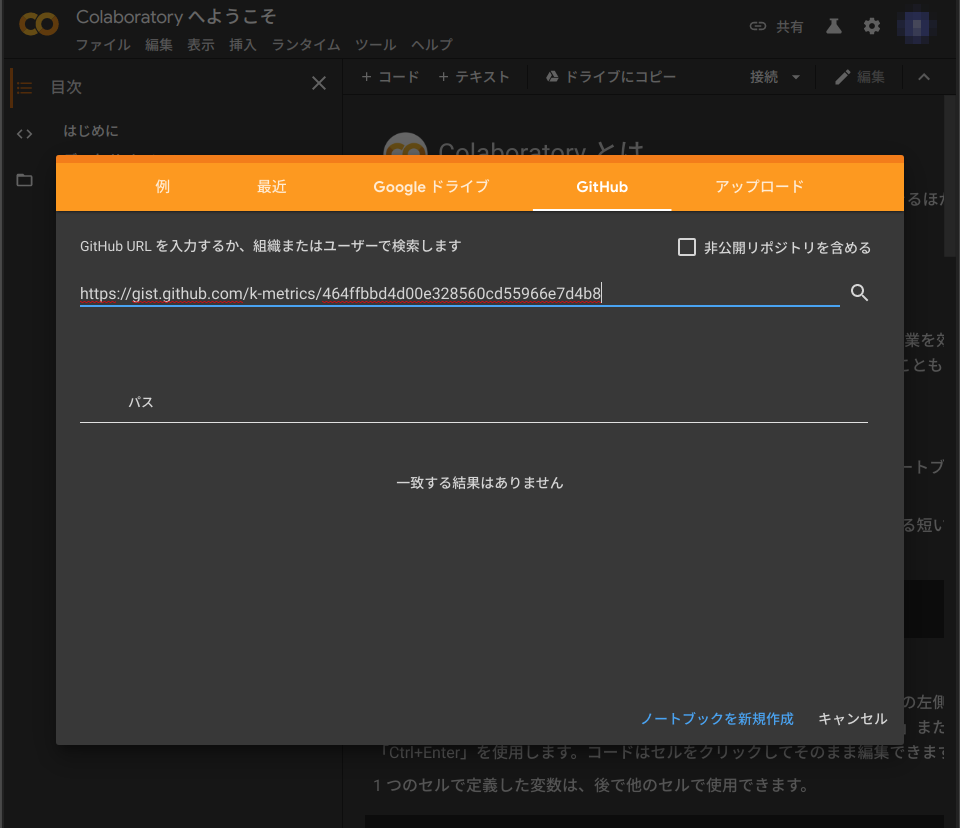
\includegraphics[width=0.8\linewidth,]{fig/Colab/upload_dialog} 

}

\caption{Upload from GitHub}\label{fig:unnamed-chunk-126}
\end{figure}

 テンプレートがアップロードされ表示されます。

 

\hypertarget{run-r-code}{%
\subsection{Run R code}\label{run-r-code}}

 テンプレートがアップロードできましたらテンプレートファイルの記述にしたがってコードを実行してみます。その際に下記のようなダイアログが表示されますが認証情報などを読み取ることはありませんので[このまま実行]をクリックしてください。

\begin{figure}[H]

{\centering 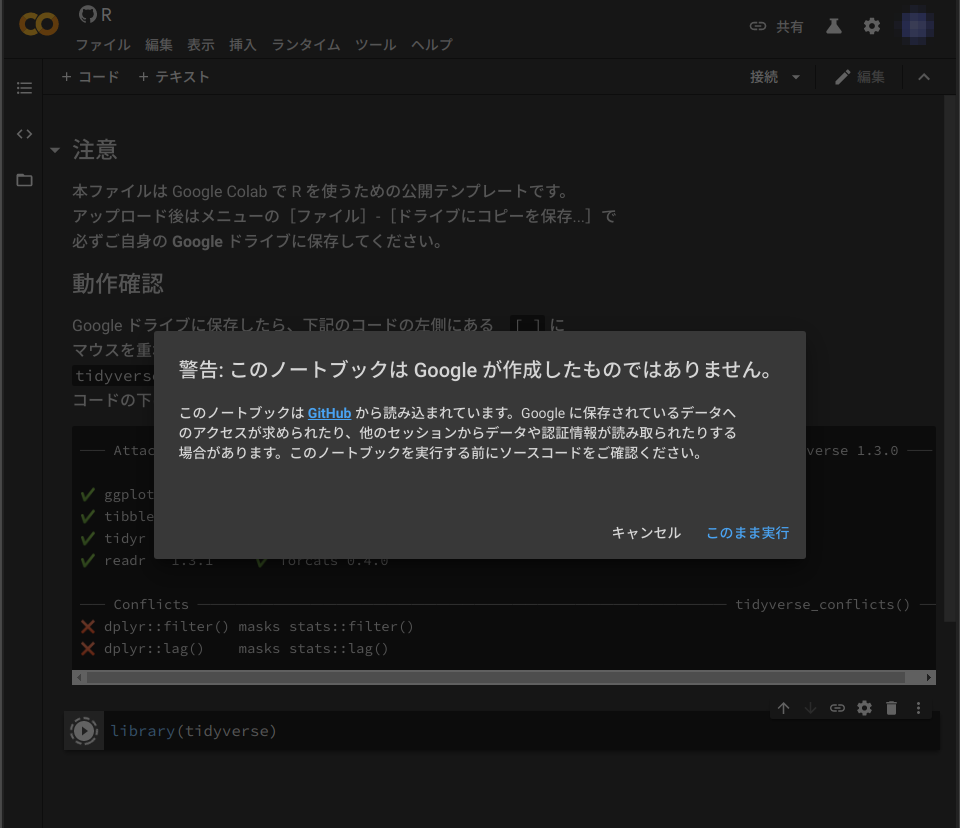
\includegraphics[width=0.8\linewidth,]{fig/Colab/run_dialog} 

}

\caption{Warning dialog}\label{fig:unnamed-chunk-127}
\end{figure}

 サーバ(ホスト型ランタイム)との接続するため実行までに多少時間がかかります。

 

\hypertarget{save-file}{%
\subsection{Save File}\label{save-file}}

 コードの実行が確認できましたらメニューの[ファイル]-[ドライブにコピーを保存\ldots]を実行してコピーを Google Drive に保存します。以降、この保存したファイルを利用してください。

 

\hypertarget{rstudio-cloud-1}{%
\section{RStudio Cloud}\label{rstudio-cloud-1}}

 Google Colab では R Markdown などのレポーティング機能は使用できませんので、このような場合には クラウド上で RStudio が利用できる RStudio Cloud が便利です。RStudio Cloud は統合開発環境の RStudio だけでなく種々のチュートリアルコンテンツを備えています。\\
 \\

\begin{figure}[H]

{\centering 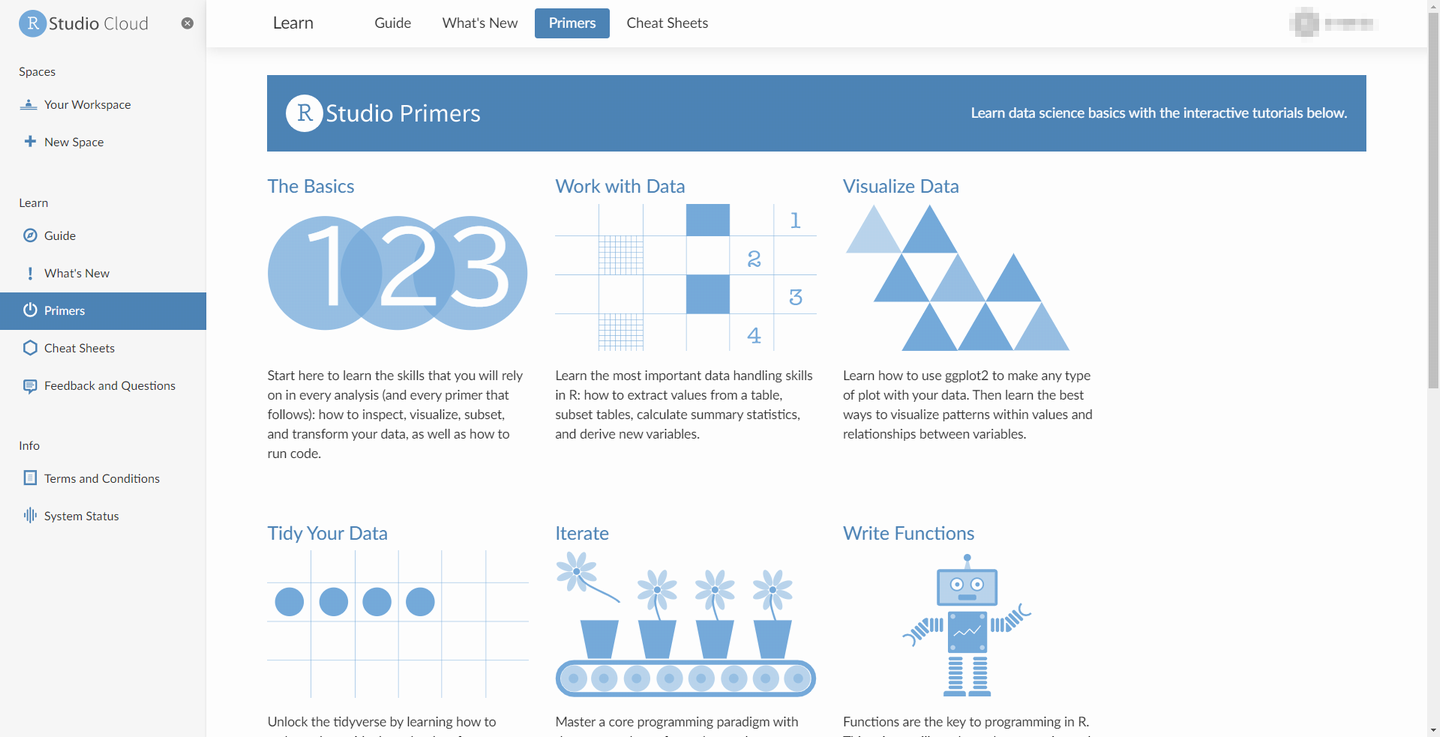
\includegraphics[width=0.8\linewidth,]{fig/RStudio/RSCloud_00} 

}

\caption{RStudio Cloud, beta}\label{fig:unnamed-chunk-128}
\end{figure}

 \\
 執筆時点では無償で利用することができ、無制限のプロジェクトとプライベートプロジェクトの作成が可能です。RStudio Cloud を利用するにはアカウントを取得するだけです。\\
 

\begin{enumerate}
\def\labelenumi{\arabic{enumi}.}
\tightlist
\item
  ブラウザで \href{https://rstudio.cloud/}{RStudio Cloud } を開く
\item
  右上の[sign up]をクリックする
\item
  RStudio Cloud のアカウントを作成してサインアップするか、Google または GitHub のアカウントでログインする
\end{enumerate}

 

\hypertarget{create-project}{%
\subsection{Create Project}\label{create-project}}

 RStudio Cloud ではプロジェクトという単位で分析を管理しますので、最初にプロジェクトを作成します。作成手順については RStudio Cloud メニューにある[Guide]で確認してください。ガイドは全て英語ですが、 Chrome 系のブラウザであれば「Google翻訳」機能拡張を用いれば日本語に翻訳表示できます。\\
 プロジェクトを作成すると下図のような統合開発環境の RStudio が表示されます。RStudio 自体の説明は Appendix を参照してください。\\
 \\

\begin{figure}[H]

{\centering 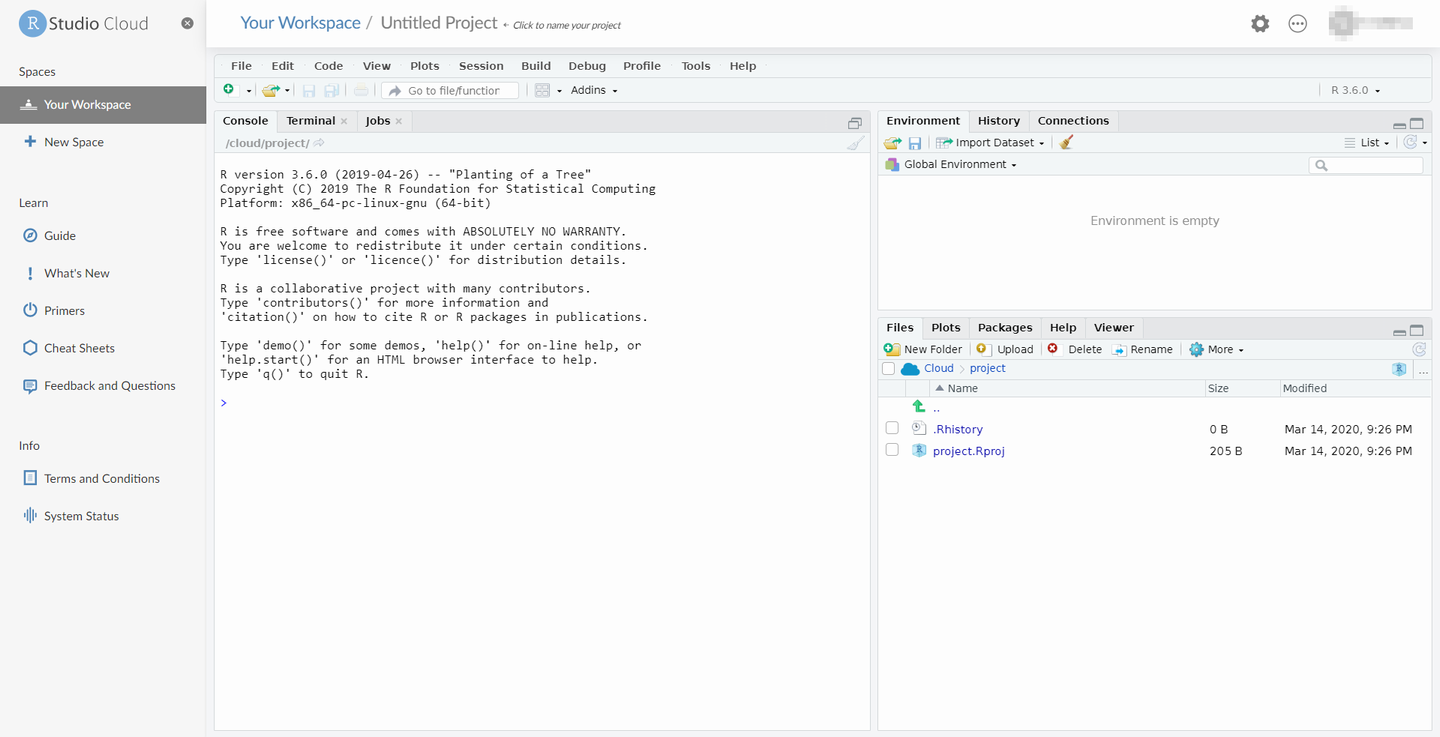
\includegraphics[width=0.8\linewidth,]{fig/RStudio/RSCloud_01} 

}

\caption{Initial View}\label{fig:unnamed-chunk-129}
\end{figure}

 

\hypertarget{install-packages}{%
\subsection{Install Packages}\label{install-packages}}

 RStudio Cloud の初期状態では R のパッケージは Base R しかインストールされていません。最も利用する \texttt{tidyverse} パッケージと \texttt{rmarkdown} パッケージをインストールするために右下のエリアにある \texttt{Packages} タブをクリックしてパッケージマネージャを表示させます。\\
 \\

\begin{figure}[H]

{\centering 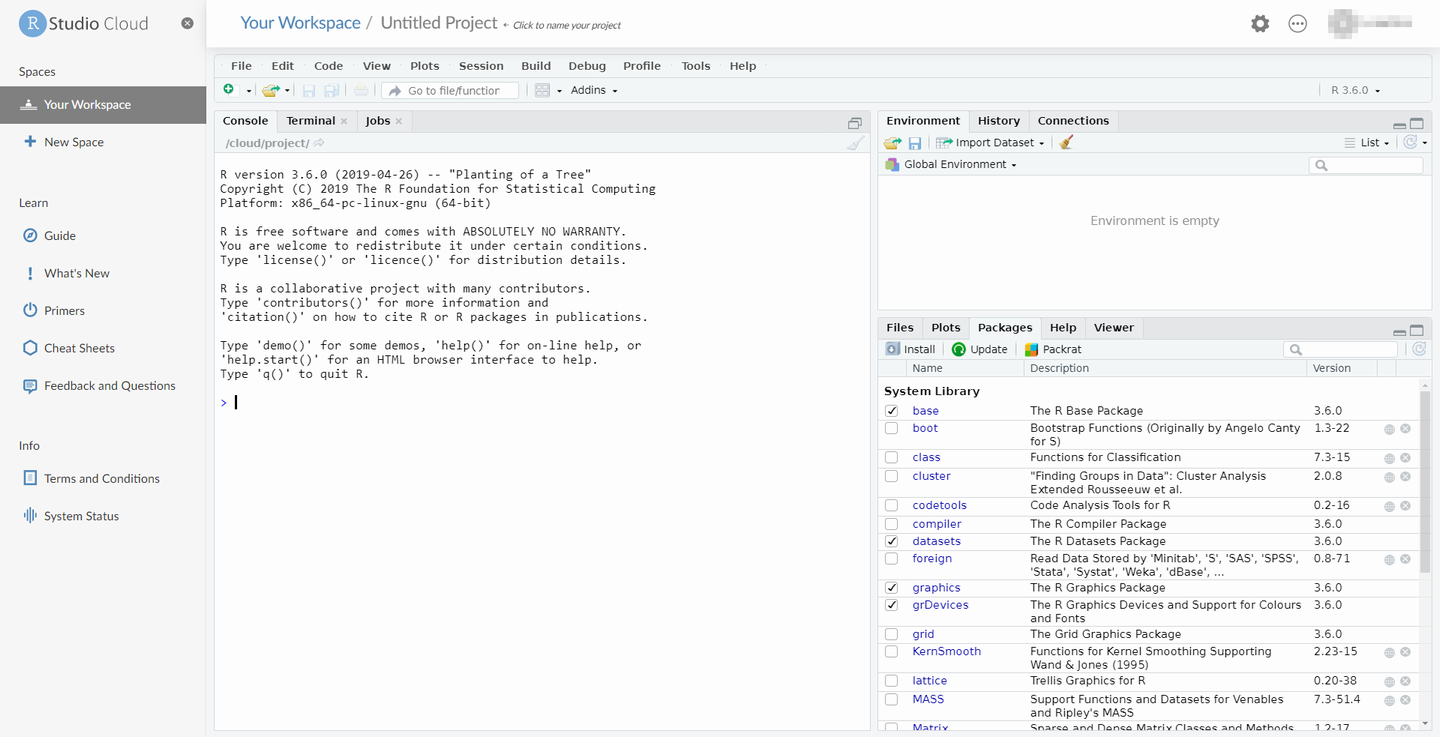
\includegraphics[width=0.8\linewidth,]{fig/RStudio/RSCloud_02} 

}

\caption{Packages Manager}\label{fig:unnamed-chunk-130}
\end{figure}

 \\
 次にパッケージマネージャの上部に表示されている \texttt{install} ボタンをクリックし表示されたダイアログに \texttt{tidyverse,\ rmarkdown} と入力し[install]ボタンをクリックしてインストールします。\\
 \\

\begin{figure}[H]

{\centering 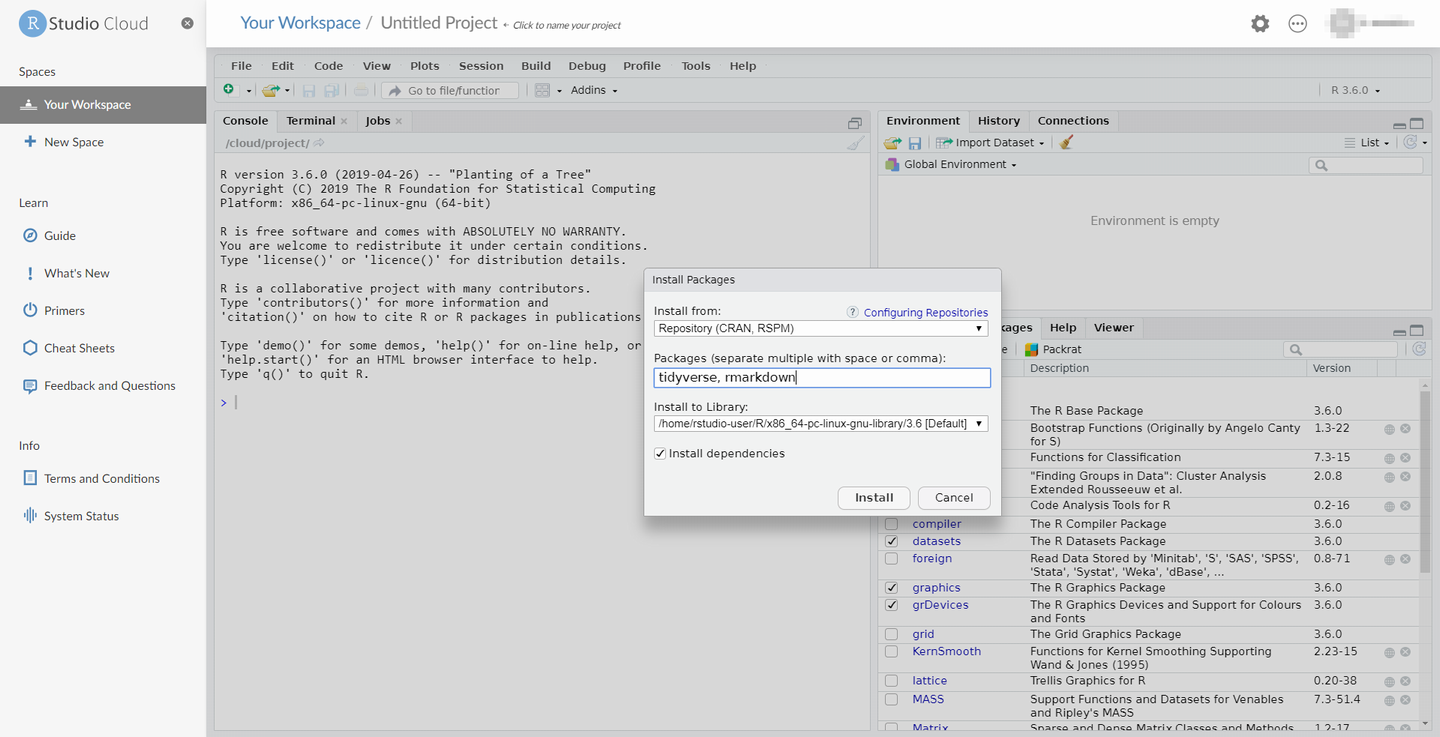
\includegraphics[width=0.8\linewidth,]{fig/RStudio/RSCloud_03} 

}

\caption{Install Dialog}\label{fig:unnamed-chunk-131}
\end{figure}

 \\
 以上で、RStudio Cloud の準備は完了です。

\hypertarget{install-rrstudio}{%
\chapter{Install R/RStudio}\label{install-rrstudio}}

 R について学ぶ前に R が使えるように環境を整えます。本書は R, RStudio, \href{https://www.tidyverse.org/}{tidyverse/ } パッケージならびにその他必要なパッケージの利用を前提としています。\\
 R ならびに RStudio はマルチプラットフォーム対応(マルチOS対応)ですので Windows, macOS, Linux のどのプラットフォームを選択しても構いません。ただし、64bit プラットフォームであることが条件です。なお、日本語版 Windows では Windows が利用してる文字コード(CP932, Shift JIS)に起因する不具合が散見されています。日本語版 Windows 環境を利用する場合はその点を認識の上で利用してください。\\
 \\
 環境を整えるための手順は以下のようになります。

\begin{longtable}[]{@{}cll@{}}
\toprule
手順 & 実施内容 & 備考 \\
\midrule
\endhead
1 & Rのインストール & 64bit プラットフォーム \\
2 & Rtoolsのインストール & Winodws のみ \\
3 & RStudioのインストール & Desktop 版 \\
4 & パッケージのインストール & tidyverse, rmarkdown \\
5 & Gitのインストール & 任意 \\
\bottomrule
\end{longtable}

 \\
 \href{https://git-scm.com/}{Git } は VCS(Version Control System) と呼ばれるソースの版管理を行うシステムです。必要な場合のみインストールしてください。

 

\hypertarget{install-r}{%
\section{Install R}\label{install-r}}

 R は \href{https://cran.r-project.org/}{CRAN (The Comprehensive R Archive Network)} と呼ばれる公式リポジトリから入手してインストールします。 CRAN には \href{https://cran.r-project.org/mirrors.html}{ミラーサイト } も多数ありますので、利用しているインターネット環境に応じて近いサイトからダウンロードしてください。\\
 よくある質問は \href{https://cran.r-project.org/doc/FAQ/R-FAQ.html}{FAQ(Frequently Asked Questions) } にまとめられています。\\
 

\hypertarget{windows}{%
\subsection{Windows}\label{windows}}

 Winodws では特段の理由がない限り \href{https://cran.r-project.org/bin/windows/}{CRAN } から最新バージョンをインストールしてください。\\
 旧バージョンをインストールしたい場合は \href{https://cran.r-project.org/bin/windows/base/old/}{Previous Releases of R for Windows } から当該バージョンをダウンロードしインストールしてください。\\
 \\
 日本語によるインストール方法が必要な場合は非公式ページですが \href{https://das-kino.hatenablog.com/entry/2019/11/07/125044}{R初心者の館(RとRStudioのインストール、初期設定、基本的な記法など) } などのサイトを参考にしてください。\\
 

\hypertarget{rtools}{%
\subsubsection{Rtools}\label{rtools}}

 Windows ではコンパイラなどの開発ツール類が標準装備されていませんので、 R のパッケージをインストールする際に必要となる Rtools と呼ばれるツールキットをインストールしておきます。 \href{https://cran.r-project.org/bin/windows/Rtools/}{Building R for Windows } のページからインストールした R のバージョン用の Rtools をダウンロードしてインストールしてください。なお、インストールの際はデフォルトオプションでインストールしてください。インストールディレクトリなどを変更すると正しく動かない場合があります。\\
 

\hypertarget{macos-os-x}{%
\subsection{macOS (OS X)}\label{macos-os-x}}

 macOS ではインストールできるバージョンが限られていますので \href{https://cran.r-project.org/bin/macosx/}{CRAN } で確認の上でインストールしてください。\\
 

\hypertarget{linux}{%
\subsection{Linux}\label{linux}}

 R がサポートしているディストリビューションは Debian, RedHat, Suse, Ubuntu のみです。Fedora を利用したい場合には \href{https://cran.r-project.org/bin/linux/redhat/README}{README } を参照の上で RedHat Software のリポジトリからインストールしてください。\\
 \\
 Linux の場合、ディストリビューションごと・バージョンごとにインストール方法が異なりますので各ディストリビューション用のディレクトリ内の README ファイルを参考にインストールしてください。\\
 

\hypertarget{install-rstudio-desktop}{%
\section{Install RStudio Desktop}\label{install-rstudio-desktop}}

 R のインストールが完了しましたら統合開発環境(IDE)である RStudio Desktop をインストールします。 \href{https://rstudio.com/products/rstudio/download/\#download}{Downloadページ } から使用している環境(OS)用の RStudio をダウンロードしてインストールしてください。  

\hypertarget{ux52d5ux4f5cux78baux8a8d}{%
\subsection{動作確認}\label{ux52d5ux4f5cux78baux8a8d}}

 RStudio のインストールが完了したら RStudio を起動します。下図のようなウィンドウが立ち上がり左側の \textbf{Console} ペインに R のバージョンなどが表示されます。\\
 \\

 \textbf{Console} ペインのプロンプト(\texttt{\textgreater{}}表示)の部分に\texttt{2\ *\ 3}と打ち込んで[Enter]キーを押し\texttt{{[}1{]}\ 6}と表示されることを確認してください。

\begin{Shaded}
\begin{Highlighting}[numbers=left,,]
\DecValTok{2} \SpecialCharTok{*} \DecValTok{3}
\end{Highlighting}
\end{Shaded}

\begin{verbatim}
[1] 6
\end{verbatim}

 

\hypertarget{install-r-packages}{%
\section{Install R packages}\label{install-r-packages}}

 次に必要となるいくつかのパッケージをインストールします。パッケージをインストールする場合はインターネットに接続されている必要があります。 \textbf{Console} ペインのプロンプトに以下のコードを入力し {[}Enter{]}キーを押して実行します。

\begin{Shaded}
\begin{Highlighting}[numbers=left,,]
\FunctionTok{install.packages}\NormalTok{(}\StringTok{"tidyverse"}\NormalTok{)}
\end{Highlighting}
\end{Shaded}

 インストールが終わりましたらパッケージが正しくインストールされていることを確認するために \textbf{Console} ペインに以下のコードを入力して実行します。

\begin{Shaded}
\begin{Highlighting}[numbers=left,,]
\FunctionTok{library}\NormalTok{(tidyverse)}
\end{Highlighting}
\end{Shaded}

 以下のようなメッセージが表示されることを確認します。インストール時期によってはバージョン表記などが下記と異なる場合があります。なお、日本語版 Windows 環境では一部の文字が化けします。

\begin{Shaded}
\begin{Highlighting}[numbers=left,,]
\NormalTok{Loading required package}\SpecialCharTok{:}\NormalTok{ tidyverse}
\NormalTok{─ Attaching packages ─────────────────────────────── tidyverse }\DecValTok{1}\NormalTok{.}\FloatTok{3.0}\NormalTok{ ─}
\NormalTok{✔ ggplot2 }\DecValTok{3}\NormalTok{.}\FloatTok{2.1}\NormalTok{     ✔ purrr   }\DecValTok{0}\NormalTok{.}\FloatTok{3.3}
\NormalTok{✔ tibble  }\DecValTok{2}\NormalTok{.}\FloatTok{1.3}\NormalTok{     ✔ dplyr   }\DecValTok{0}\NormalTok{.}\FloatTok{8.3}
\NormalTok{✔ tidyr   }\DecValTok{1}\NormalTok{.}\FloatTok{0.0}\NormalTok{     ✔ stringr }\DecValTok{1}\NormalTok{.}\FloatTok{4.0}
\NormalTok{✔ readr   }\DecValTok{1}\NormalTok{.}\FloatTok{3.1}\NormalTok{     ✔ forcats }\DecValTok{0}\NormalTok{.}\FloatTok{4.0}
\NormalTok{─ Conflicts ───────────────────────────────── }\FunctionTok{tidyverse\_conflicts}\NormalTok{() ─}
\NormalTok{✖ dplyr}\SpecialCharTok{::}\FunctionTok{filter}\NormalTok{() masks stats}\SpecialCharTok{::}\FunctionTok{filter}\NormalTok{()}
\NormalTok{✖ dplyr}\SpecialCharTok{::}\FunctionTok{lag}\NormalTok{()    masks stats}\SpecialCharTok{::}\FunctionTok{lag}\NormalTok{()}
\end{Highlighting}
\end{Shaded}

 

 続いて \href{https://rmarkdown.rstudio.com/}{rmarkdown } パッケージをインストールします。\texttt{tidyverse} パッケージのときと同様に以下のコードを \textbf{Console} ペインに入力して実行します。

\begin{Shaded}
\begin{Highlighting}[numbers=left,,]
\FunctionTok{install.packages}\NormalTok{(}\StringTok{"rmarkdown"}\NormalTok{)}
\end{Highlighting}
\end{Shaded}

\hypertarget{linuxux74b0ux5883ux306eux5834ux5408}{%
\subsection{Linux環境の場合}\label{linuxux74b0ux5883ux306eux5834ux5408}}

 Linux環境ではプラットフォーム側のライブラリなどが足りずにパッケージのインストールが完了できない場合があります。その場合は \href{https://demo.rstudiopm.com/client/\#/}{RStudio Package Manager, demo site } にてインストールしたいパッケージが必要とするライブラリなどを確認、インストールしてから再度パッケージをインストールしてください。\\
 例えば Ubuntu 18.04LTS で R に \texttt{tidyverse} パッケージをインストールする場合には以下のようなライブラリなどがOS側にインストールされている必要があります。\\
 

\begin{Shaded}
\begin{Highlighting}[numbers=left,,]
\ExtensionTok{apt{-}get}\NormalTok{ install }\AttributeTok{{-}y}\NormalTok{ libicu{-}dev}
\ExtensionTok{apt{-}get}\NormalTok{ install }\AttributeTok{{-}y}\NormalTok{ make}
\ExtensionTok{apt{-}get}\NormalTok{ install }\AttributeTok{{-}y}\NormalTok{ libcurl4{-}openssl{-}dev}
\ExtensionTok{apt{-}get}\NormalTok{ install }\AttributeTok{{-}y}\NormalTok{ libssl{-}dev}
\ExtensionTok{apt{-}get}\NormalTok{ install }\AttributeTok{{-}y}\NormalTok{ pandoc}
\ExtensionTok{apt{-}get}\NormalTok{ install }\AttributeTok{{-}y}\NormalTok{ libxml2{-}dev}
\end{Highlighting}
\end{Shaded}

 

\hypertarget{install-git}{%
\section{Install Git}\label{install-git}}

 RStudio にはソースコードの版管理を行うインタフェースが標準で用意されていますが、版管理システム(以降、VCS)を別途インストールする必要があります。RStudio で利用できる VCS は以下の二つです。\\
 

\begin{itemize}
\tightlist
\item
  \href{https://git-scm.com/}{Git }
\item
  \href{https://subversion.apache.org/}{Subversion(SVN) }
\end{itemize}

 どちらを利用しても構いませんが \href{https://github.com/}{GitHub } などのクラウドサービスが充実している Git の利用をおすゝめします。\\
 

\hypertarget{git}{%
\subsection{Git}\label{git}}

 Windows および macOS は Gitの \href{https://git-scm.com/downloads}{ダウンロードページ } から最新バージョンをダウンロードしてインストールします。Linux はリポジトリからインストールするか \href{https://git-scm.com/downloads}{ダウンロードページ } から最新バージョンをダウンロードしてインストールしてください。\\
 

\hypertarget{git-client}{%
\subsection{Git Client}\label{git-client}}

 RStudio には簡易的な Git のクライアント機能が標準で用意されていますが、きめ細かな操作を行いたい場合には Git の GUI クライアントをインストールしてください。代表的な Git Client を以下に列挙しておきます。\\
 

\begin{longtable}[]{@{}lcccl@{}}
\toprule
Git GUI Client & Ubuntu & Mac & Windows & Memo \\
\midrule
\endhead
\href{https://www.gitkraken.com/}{GitKraken } & Yes & Yes & Yes & Free版は機能制限あり \\
\href{https://www.syntevo.com/smartgit/}{SmartGit } & Yes & Yes & Yes & Free版でも機能制限なし\textsuperscript{1} \\
\href{https://www.collab.net/downloads/giteye}{GitEye } & Yes & Yes & Yes & \\
\href{https://www.sourcetreeapp.com/}{Sourcetree } & No & Yes & Yes & 日本語版あり \\
\href{https://desktop.github.com/}{GitHub Desktop } & No & Yes & Yes & \\
\bottomrule
\end{longtable}

\textsuperscript{1} : 非商用利用の場合

 

\hypertarget{rstudio-server}{%
\chapter{RStudio Server}\label{rstudio-server}}

 R/Rstudio Desktop は前述のようにマルチプラットフォーム対応ですがプラットフォームごとに以下のような制約があります。\\
 

\begin{itemize}
\tightlist
\item
  日本語版 Windows 環境では文字コード(CP932, Shift JIS)が原因で日本語を正しく処理できない事例が散見される
\item
  18.04LTSより前の Ubuntu 環境では RStudio Desktop で日本語入力ができない * 有志による日本語入力パッチ(非公式パッチ)はあり
\item
  macOS 環境ではグラフの日本語が文字化けする * いわゆる豆腐文字問題
\end{itemize}

 \\
 特に日本語版 Windows 環境での問題は Windows が利用している文字コード(CP932, Shift JIS) に起因しているため問題は根本的な解決を期待できません。詳細については伝説とも言われている「Why are you using SJIS?」というキーワードで検索してみてください。\\
 \\
 日本語版 Windows 環境における文字コード問題を回避するためには、 \href{https://rstudio.com/products/rstudio/download-server/}{RStudio Server } を利用する方法が考えられます。  RStudio Server は Linux 環境で動作する Web サーバベースの IDE ですが、 \href{https://www.docker.com/}{Docker } のコンテナ技術を利用することで Windows や macOS 環境で動作させることが可能です。  

\begin{longtable}[]{@{}
  >{\raggedright\arraybackslash}p{(\columnwidth - 4\tabcolsep) * \real{0.14}}
  >{\raggedright\arraybackslash}p{(\columnwidth - 4\tabcolsep) * \real{0.50}}
  >{\raggedright\arraybackslash}p{(\columnwidth - 4\tabcolsep) * \real{0.36}}@{}}
\toprule
\begin{minipage}[b]{\linewidth}\raggedright
OS
\end{minipage} & \begin{minipage}[b]{\linewidth}\raggedright
Docker app
\end{minipage} & \begin{minipage}[b]{\linewidth}\raggedright
System Requirements
\end{minipage} \\
\midrule
\endhead
macOS & Docker Desktop for Mac & \href{https://docs.docker.com/docker-for-mac/install/}{refer docker docs } \\
Windows & Docker Desktop for Windows & Hyper-V(Windows10 64bit Pro or Higher) or WSL2\textsuperscript{1} \\
\bottomrule
\end{longtable}

 \\
\textsuperscript{1} WSL2 は Windows10 version 2004 から利用可能になる予定です

 

\hypertarget{setup-rstudio-sever-with-docker}{%
\section{Setup RStudio Sever with Docker}\label{setup-rstudio-sever-with-docker}}

 Windows または macOS 環境で Docker を利用し RStudio Server を起動するためには以下の手順が必要です。\\
 

\begin{longtable}[]{@{}cll@{}}
\toprule
手順 & 実施内容 & 備考 \\
\midrule
\endhead
1 & Hyper-V の有効化 & Windows のみ \\
2 & Docker Desktop のインストール & \\
3 & Docker Image のダウンロード & \\
4 & Docker Container の起動 & \\
\bottomrule
\end{longtable}

 \\
 なお、Linux 環境での手順は割愛します。  

\hypertarget{enable-hyper-v-windows-only}{%
\subsection{Enable Hyper-V (Windows Only)}\label{enable-hyper-v-windows-only}}

 Windows 環境ではインストールする前に \href{https://docs.microsoft.com/ja-jp/virtualization/hyper-v-on-windows/quick-start/enable-hyper-v}{Hyper-V を有効にする } 必要があります。

\hypertarget{download-and-install-docker-desktop}{%
\subsection{Download and Install Docker Desktop}\label{download-and-install-docker-desktop}}

 利用している環境に応じた \href{https://www.docker.com/products/docker-desktop}{Docker Desktop } をダウンロードしてインストールします。なお、ダウンロードには \href{https://hub.docker.com/}{docker hub } でアカウント登録が必要です。\\
 \\
 詳細な手順や設定方法は \href{https://docs.docker.com/get-docker/}{Docker docs } を参照してください。\\
 

\hypertarget{download-docker-image}{%
\subsection{Download Docker Image}\label{download-docker-image}}

 Docker Desktop をインストール・起動しましたら RStudio Server の Docker Image をダウンロードします。様々な方が RStudio Server の Docker Image を公開されていますが代表的な Docker Image には次のようなものがあります。\\
 

\begin{longtable}[]{@{}ll@{}}
\toprule
Image & Description \\
\midrule
\endhead
\href{https://hub.docker.com/r/rocker/tidyverse}{rocker/tidyverse } & Version-stable base R and RStudio, tidyverse, devtools \\
\href{https://hub.docker.com/r/rocker/verse}{rocker/verse } & Adds TeX and related packages to rocker/tidyverse \\
\href{https://hub.docker.com/r/ykunisato/paper-r-jp}{ykunisato/paper-r-jp } & Dockerfile of writing paper by R Markdown \\
\href{https://hub.docker.com/r/kmetrics/jverse}{kmetrics/jverse } & Japanized rocker/verse \\
\bottomrule
\end{longtable}

 \\
 \href{https://github.com/rocker-org/rocker}{rocker } は準公式とも言えるような R に関連する Docker Image を継続的に提供しているプロジェクトです。様々なイメージを提供していますが残念ながら日本語フォントの追加などの日本語対応がなされていません。グラフで日本語を利用しない限りは rocker のイメージを利用しても何ら問題はありません(ソースなどの表示はブラウザに依存しているのでコードに日本語を記述することが可能です)。\\
 グラフで日本語を利用したい場合は著者が rocker/verse に日本語フォントなどを追加して日本語対応させた \href{https://hub.docker.com/r/kmetrics/jverse}{kmetrics/jverse } を利用するか rocker が公開している Dockerfile を改修して日本語対応させたイメージを利用してください。\\
 \\
 利用する Docker Image を決めたらコンソール(コマンドプロンプト)で以下のコマンドを実行してイメージをダウンロードしてください。\\
 

\begin{Shaded}
\begin{Highlighting}[numbers=left,,]
\ExtensionTok{docker}\NormalTok{ pull rocker/tidyverse}
\end{Highlighting}
\end{Shaded}

 

\hypertarget{run-container}{%
\subsection{Run Container}\label{run-container}}

\hypertarget{rstudio-ide}{%
\chapter{RStudio IDE}\label{rstudio-ide}}

 データ分析勉強会では長らく \href{https://www.rcommander.com/}{R Commander(以降、Rcmdr) } が利用されています。勉強会の母体となっている \href{https://www.juse.or.jp/sqip/workshop/outline/index.html}{SQiP研究会 } のソフトウェアメトリクスに関する演習コースでも同様です。これはプログラミングに縁の薄いソフトウェア品質管理技術者が短期間で R を用いた分析を行えるようにとの配慮からです。実際、 Rcmdr はコードを記述しなくてもデータの可視化や分析ができますのでデータ分析の初学者にとっては R の恩恵を簡単に受けられる非常に便利な道具です。\\
 しかし、Rcmdr は R のごく一部の関数を GUI で使えるようにしたラッパープログラムですので、できることが非常に限られています。加えて GUI 操作なため操作自体が記録に残りません。つまり、探索的にデータを分析を行ってもその手順分析者の記憶に依存してしまいますので分析再現性の観点から見ると好ましい分析環境とは言えません。\\
 \\
 本格的な探索的データ分析を行うには、出来ることが限られる Rcmdr ではなく R のスクリプトを用いるべきです。しかし、 R 本体(R Console)は非常に機能が限られていますので、それだけで探索的データ分析を行うのは非常に困難です。そこで、初学者には様々な機能を予め備えている統合開発環境(IDE - Integrated Development Environment)を利用をおすゝめします。\\
 \\
 R 用統合開発環境のデファクトスタンダードと言えるのが RStudio, PBC の \href{https://rstudio.com/products/rstudio/}{RStudio IDE (以降、RStudio)} です。無償版である Open Source Edition でも全ての基本的な機能を利用できます。\\
 \\
 初学者にとって RStudio には以下のような便利な機能があります。

\begin{itemize}
\tightlist
\item
  補完機能が強力

  \begin{itemize}
  \tightlist
  \item
    関数名・変数名・パッケージ名などを補完してくれますので入力負荷が大幅に減ります
  \end{itemize}
\item
  エディタ機能が強力

  \begin{itemize}
  \tightlist
  \item
    キーひとつでヘルプの参照が可能ですので即座に疑問が解決できます
  \item
    部分的にコードを実行できますので手順を確認しながらコーディングできます
  \item
    Markdown 記述が使えますので分析と報告書作成を同時に進められます

    \begin{itemize}
    \tightlist
    \item
      コードの直下に実行結果を表示することができますのでコードと実行結果の関係性が一目でわかります
    \end{itemize}
  \end{itemize}
\item
  パッケージ管理が分かりやすい

  \begin{itemize}
  \tightlist
  \item
    インストールされているパッケージが一目でわかります
  \item
    パッケージの検索・読込み・インストールが GUI 操作で簡単にできます
  \end{itemize}
\item
  その他の便利な機能

  \begin{itemize}
  \tightlist
  \item
    作成した変数を一覧で確認できると共に値も確認できます
  \item
    プロジェクト管理機能が使えますので分析ごとにファイルなどをセパレートできます
  \item
    バージョンコントロールシステムを用いた履歴管理ができます
  \item
    Python などの他言語もサポートしています
  \end{itemize}
\end{itemize}

 上記は機能のほんの一部を紹介したにすぎません。 RStudio は R を利用した探索的データ分析を効率的かつ強力にしかも無償でサポートしてくれる道具です。\\
 

\hypertarget{overview}{%
\section{Overview}\label{overview}}

 RStudio を起動すると以下のような画面が表示されます。画面は大きく以下の四つのエリアに分割されており、左上の A のエリアはソースエディタが表示されるエリアなので初めて起動した際には表示されません。\\
 

\begin{figure}[H]

{\centering 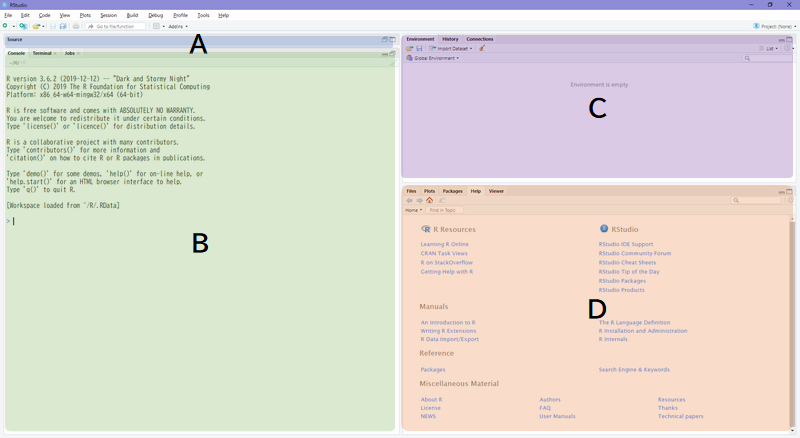
\includegraphics[width=0.8\linewidth,]{fig/RStudio/DT_Area} 

}

\caption{RStudio Desktop, Windows}\label{fig:unnamed-chunk-139}
\end{figure}

 各エリアのサイズ(ウィンドウ内での比率)は任意に調整できますが、横幅に関しては A と B 、 C と D が常に同サイズとなります。各エリアにはペインと呼ばれるタブ切り替え型のサブエリアが表示されます。ペインは常時表示されるペイン(下図の黒文字)と機能が呼び出されたり利用を設定している場合にのみ表示されるペイン(下図の灰文字)があります。

\begin{figure}[H]

{\centering 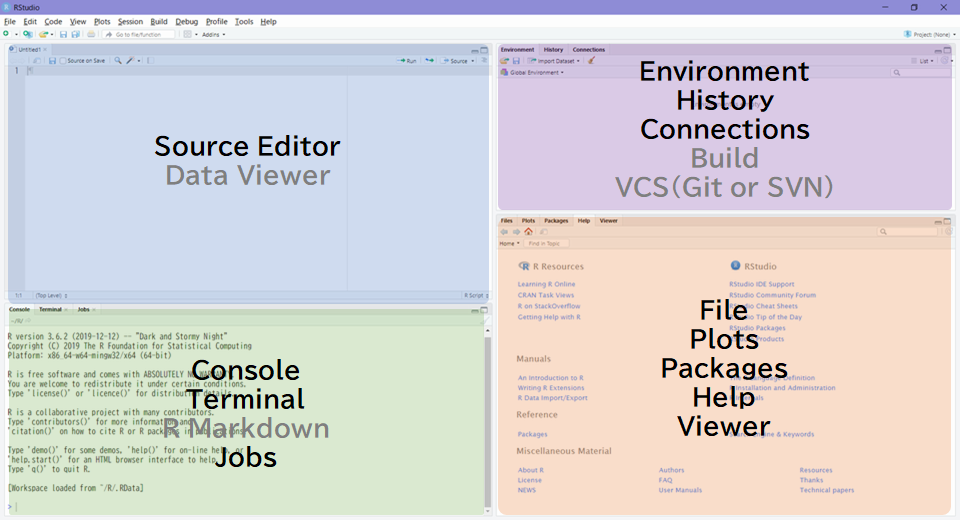
\includegraphics[width=0.8\linewidth,]{fig/RStudio/DT_Pane} 

}

\caption{RStudio Pane Layout, Windows}\label{fig:unnamed-chunk-140}
\end{figure}

 RStudio のバージョンにより多少ペイン構成が異なりますが以下のペインが用意されています。これらのペインはグローバルオプションで表示位置の変更や表示・非表示の切り替えができます。\\
 

\begin{longtable}[]{@{}clll@{}}
\toprule
No & Area & Pane name & Descriptions \\
\midrule
\endhead
1 & A & (File name) & ソースエディタ(ファイルが開かれていない場合は未表示) \\
2 & A & (Data name) & データフレーム型の変数などを表示するデータビューア \\
3 & B & Console & 文字通りRのコンソール(実行結果の表示だけでなくここから実行することも可) \\
4 & B   & Terminal & OS のターミナル(RStudio v1.1から) \\
5 & B & R Markdown & R Markdown ファイルをレンダリングした際にレンダリング情報を表示 \\
6 & B   & Jobs & ローカルジョブの実行マネージャ(RStudio v1.2から) \\
7 & C & Environment & オブジェクト(変数、関数)の表示と参照ができる環境マネージャ \\
8 & C & History & 実行履歴マネージャ(コンソールでの実行、ソースからの実行共に記録) \\
9  & C & Connections & データソース接続マネージャ(RStudio v1.1から) \\
10 & C & Build & ビルドツール(プロジェクトオプションで有効にしている場合のみ) \\
11 & C & Git or SVN & 簡易VCSクライアント(プロジェクトオプションでVCSを有効にしている場合のみ) \\
12 & D & Files & 簡易なファイルマネージャ \\
13 & D & Plots & グラフィック専用プロットエリア(ヒストリ機能、出力機能付き) \\
14 & D & Packages & パッケージ管理を行うためのパッケージマネージャ \\
15 & D & Help & ヘルプビューア(ソースエディタやコンソールと連動したヘルプ表示が可) \\
16 & D & Viewer & HTML等の表示が可能なビューア \\
\bottomrule
\end{longtable}

 

\hypertarget{keyboard-shortcuts}{%
\section{Keyboard Shortcuts}\label{keyboard-shortcuts}}

 キーボードショートカットは効率的なコーディングに役立ちますので、最低限、以下のショートカットを覚えましょう。\\
 

\begin{longtable}[]{@{}ll@{}}
\toprule
Keyboard Shortcuts & Description \\
\midrule
\endhead
[TAB] & 入力中のコード(オブジェクト)を補完 \\
[Alt/Option]+[-] & 代入演算子(\texttt{\textless{}-})をカーソル位置に挿入する \\
[Ctrl/Cmd]+[Shift]+[M] & パイプ演算子(\texttt{\%\textgreater{}\%})をカーソル位置に挿入する \\
[Ctrl/Cmd]+[Shift]+[C] & 選択行をコメント・アンコメントする(トグル動作) \\
[Ctrl/Cmd]+[Alt/Option]+[I] & カーソル位置にコードチャンクを挿入する(R Markdownのみ) \\
[Ctrl/Cmd]+[Enter] & 選択したコードを実行する(行選択、部分選択どちらも可) \\
[Ctrl/Cmd]+ {[}Shift{]} +[Enter] & コードチャンク内の全てのコードを実行する(R Markdownのみ) \\
[F1] & 選択またはカーソル位置の関数のヘルプを呼び出す \\
[Ctrl/Cmd]+[F] & アクティブなペイン内の検索 \\
\bottomrule
\end{longtable}

 \\
 上記以外のショートカットはメニュー[\textbf{Tools}]-[\textbf{Keyboard Shortcuts Help}]を選択すると表示できます。\\
 

\hypertarget{writing-r-code}{%
\section{Writing R code}\label{writing-r-code}}

 では、実際に RStudio を利用して簡単なコードを書いてみましょう。初学者が学習のために R のコードを記述するには R Notebook 形式が便利です。 R Notebook 形式は マークダウン言語とコードを混在できる R Markdown 形式を簡易にしたものです。コード以外に説明などを記述できるのでアウトプットしながらの学習が可能です。  R Notebook 形式を使うにはメニューから[File]-[New File]-[R Notebook]を実行します。すると下図のようなソースエディタ(以降、エディタ)が開きます。

\begin{figure}[H]

{\centering 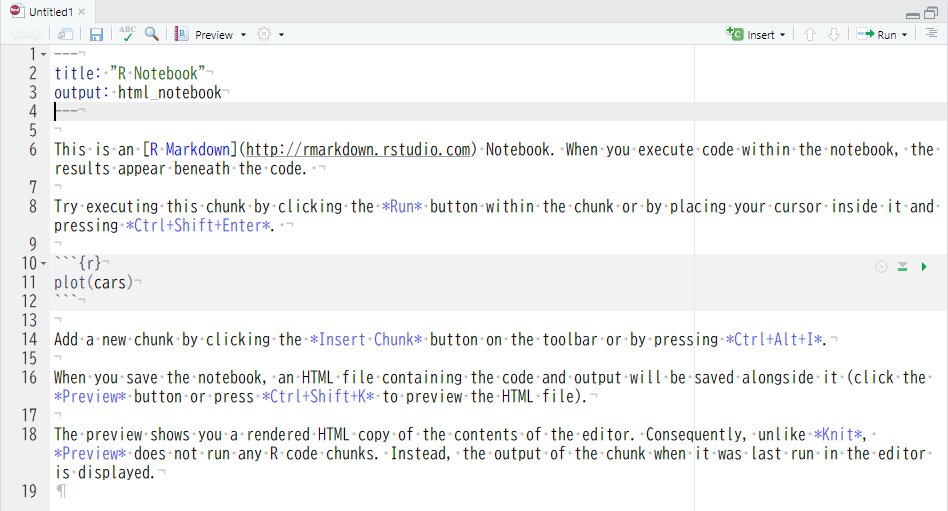
\includegraphics[width=0.8\linewidth,]{fig/RStudio/DT_RN} 

}

\caption{R Notebook file}\label{fig:unnamed-chunk-141}
\end{figure}

 この時点ではファイルとして保存されていませんので、メニューから[File]-[Save As\ldots]を実行して適当な場所に適当な名前で保存しておきます。ここでは \texttt{test} という名前を入力して保存します。ファイルの拡張子が自動的に付与されますのでタブの表示は \texttt{test.Rmd} となります。

\begin{figure}[H]

{\centering 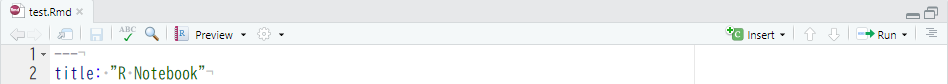
\includegraphics[width=0.8\linewidth,]{fig/RStudio/DT_RN_Saved} 

}

\caption{R Notebook saved file}\label{fig:unnamed-chunk-142}
\end{figure}

 ファイルを保存したら 6 行目の「This is an \ldots」から 18 行目の「in the editor is displayed.」までを削除し、カーソルの位置(6 行目)でキーボードショートカット[Ctrl/Cmd]+[Alt/Option]+[I]を押下してコードを記述するためのブロックを挿入します。

\begin{figure}[H]

{\centering 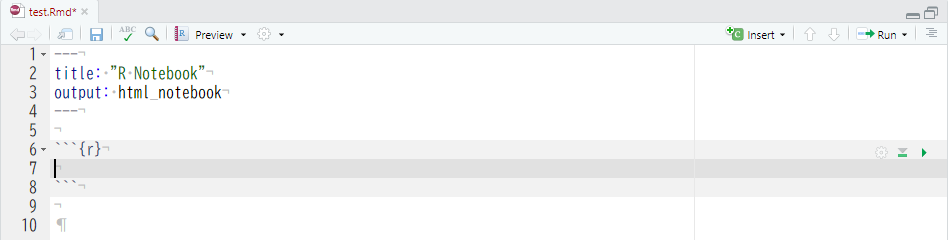
\includegraphics[width=0.8\linewidth,]{fig/RStudio/DT_RN_Insert_Chunk} 

}

\caption{R Notebook insert chunk}\label{fig:unnamed-chunk-143}
\end{figure}

 すると上図のように三連のバッククォート(\texttt{\textasciigrave{}\textasciigrave{}\textasciigrave{}})で囲まれたブロックが挿入されます。このブロックはコードチャンクと呼ばれる R のコードを記述する部分です。コードチャンクの前後は自由な記述が出来ますので、以下のように入力してみてください。

\begin{figure}[H]

{\centering 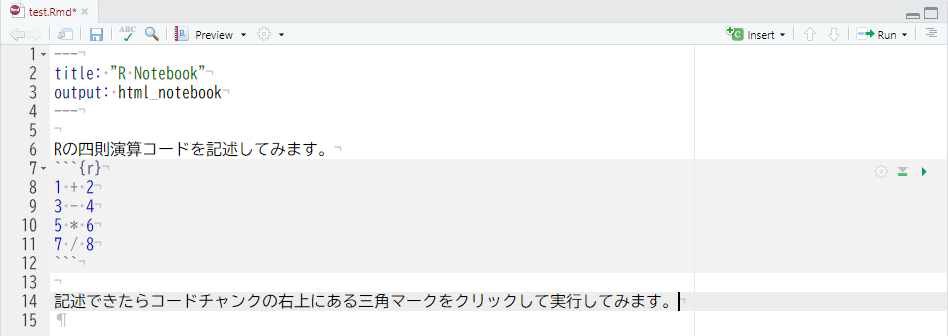
\includegraphics[width=0.8\linewidth,]{fig/RStudio/DT_RN_First_Code} 

}

\caption{R Notebook first code}\label{fig:unnamed-chunk-144}
\end{figure}

 上図のように R Notebook では説明とコードを混在することができます。では、コードチャンクの右上にある緑色の三角マークをクリックしてコードを実行してみましょう。

\begin{figure}[H]

{\centering 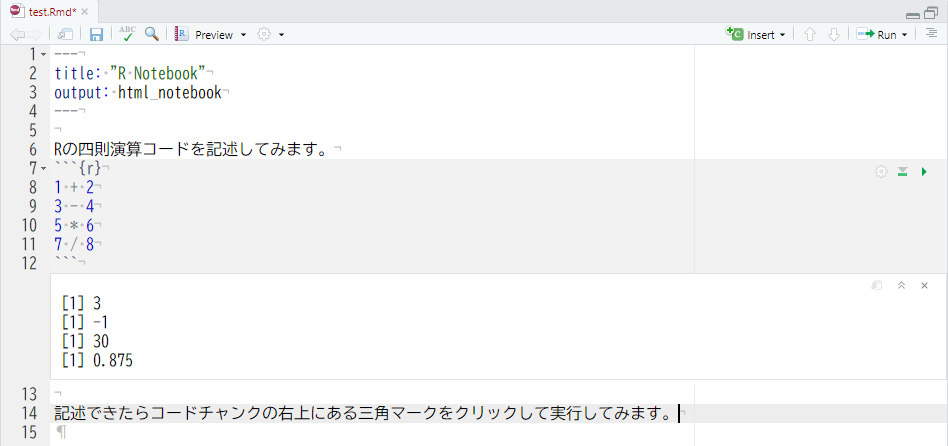
\includegraphics[width=0.8\linewidth,]{fig/RStudio/DT_RN_Run_Code} 

}

\caption{R Notebook run code}\label{fig:unnamed-chunk-145}
\end{figure}

 コードチャンクの下と \textbf{Console} ペインに実行結果が表示されます。コードチャンクの下に実行結果が表示されない場合は下図のように歯車アイコンをクリックし表示したメニューから \texttt{Chunk\ Output\ Inline} にチェックをつけ、再度、緑色の三角マークをクリックしてコードを実行してください。コードチャンクの下に実行結果が表示されます。

\begin{figure}[H]

{\centering 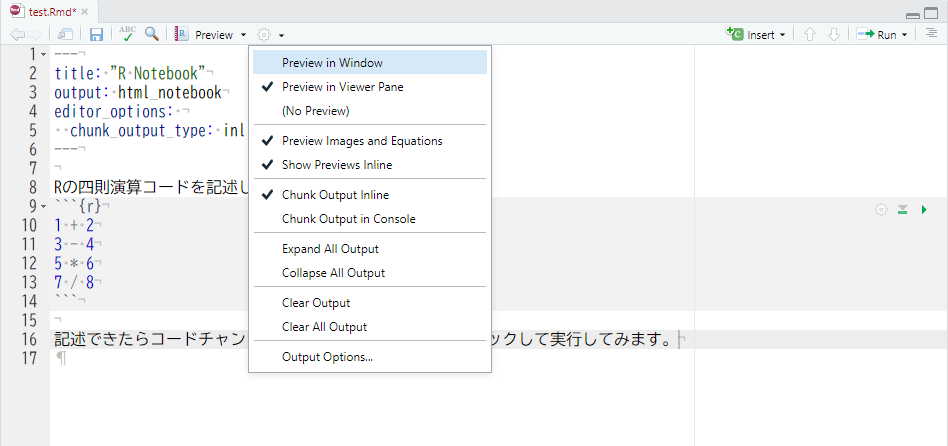
\includegraphics[width=0.8\linewidth,]{fig/RStudio/DT_RN_Option} 

}

\caption{R Notebook option}\label{fig:unnamed-chunk-146}
\end{figure}

 最後にフロッピーディスクアイコンをクリックするかキーボードショートカットの[Ctrl/Cmd]+[S]を押下してファイルを保存しておきます。

\hypertarget{global-options}{%
\section{Global Options}\label{global-options}}

 メニュー[\textbf{Tools}]-[\textbf{Global Options\ldots{}}]を選択すると表示できます。以降に推奨設定項目を記載しておきますので参考にしてください。記載されていないオプションはお好みで設定してください。\\
 

\hypertarget{general}{%
\subsection{General}\label{general}}

 Genelal オプションは RStudio の全般的な動作に関する設定です。 Basic と Advanced の二種類の設定がありますが、初学者の方は Basic のみ以下のように設定しておくと便利です。\\
 

\begin{longtable}[]{@{}llll@{}}
\toprule
大項目(Tab) & 中項目(太文字) & 設定項目 & 推奨設定 \\
\midrule
\endhead
Basic & R Sessions & R version & Default(Windows only) \\
Basic & R Sessions & Default working directory & 任意のディレクトリ \\
Basic & R Sessions & Restore most recently opened project at startup & Unchecked \\
Basic & Workspace & Restore .RData into workspace at startup & Checked \\
Basic & Wrokspace & Save workspace to .RData on exit & ``Ask'' or ``Always'' \\
Basic & Ohter & Automatically notify me of updates to RStudio & Checked \\
\bottomrule
\end{longtable}

 \\
 特に ``Default working directory'' はプロジェクトを作成・管理するディレクトリに設定しておくと便利です。

 

\hypertarget{code}{%
\subsection{Code}\label{code}}

 Code オプションはソースエディタの動作に関する設定です。ソースの記述は \href{https://style.tidyverse.org/}{スタイルガイド(The tidyverse style guide) } に準拠することをおすゝめしますので、設定例もスタイルガイドに沿ったものになっています。なお、 Python などの他言語を併用する場合は適切な設定に変更してください。\\
 

\begin{longtable}[]{@{}llll@{}}
\toprule
大項目(Tab) & 中項目(太文字) & 設定項目 & 推奨設定 \\
\midrule
\endhead
Editing & General & Insert spaces for tab & Checked \\
Editing & General & Tab width & 2 \\
Editing & General & Auto-detect code indentation & Checked \\
Editing & General & Insert matching parens/quotes & Checked \\
Editing & General & Auto-indent code after paste & Checked \\
Editing & General & Vertically align arguments in atuo-indent & Checked \\
Editing & General & Surround selection on text insertion & ``Quotes \& Brackets'' \\
Editing & Execution & Always save R scripts before sourcing & Checked \\
Editing & Execution & Ctrl+Enter executes & ``Multi-line R statement'' \\
Display & General & Highlight selected word & Checked \\
Display & General & Highlight selected line & Checked \\
Display & General & Show line numbers & Checked \\
Display & General & Show margin & Checked \\
Display & General & Margin coloumn & 80 \\
Display & General & Show whitespace characters & Checked \\
Display & General & Show syntax highlighting in console input & Checked \\
Saving & General & Restore last cursor position when opening file & Checked \\
Saving & Serialization & Line ending conversion & ``Posix (LF)'' \\
Saving & Serialization & Default text encoding & ``UTF-8'' \\
\bottomrule
\end{longtable}

 

\hypertarget{appearance}{%
\subsection{Appearance}\label{appearance}}

 Appearance オプションは RStudio の見た目に関する設定です。フォント設定のみ日本語の固定ピッチフォントに変更し、その他はお好みでどうぞ。\\
 

\begin{longtable}[]{@{}llll@{}}
\toprule
大項目(Tab) & 中項目(太文字) & 設定項目 & 推奨設定 \\
\midrule
\endhead
N/A & N/A & Editor font & 任意の日本語等幅フォント \\
\bottomrule
\end{longtable}

 \\
 日本語等幅フォントは好みで構いませんが、無償ダウンロード可能な以下のフォントがおすゝめです。

\begin{itemize}
\tightlist
\item
  BIZ UDゴシック(macOS, Windows) - MORISAWA PASSPORT
\item
  Source Han Code JP(Linux, macOS) - SIL Open Font License
\item
  IPAゴシック(Linux, macOS, Windows) - IPA フォントライセンス
\end{itemize}

 なお、日本語版 Windows の RStudio では一部の日本語等幅フォントを正しく表示できないバグがあるようですので、フォントの選択には注意してください。

 

\hypertarget{pane-layout}{%
\subsection{Pane Layout}\label{pane-layout}}

 Pane Layout オプションは前述のペインの表示場所や表示・非表示を変更するためのオプションですので、初学者はデフォルト設定のまま利用することをおすゝめします。

 

\hypertarget{packages}{%
\subsection{Packages}\label{packages}}

 Packages オプションはパッケージマネジメントに関する設定です。 Management と Development の二種類の設定がありますが、Development はパッケージ自体を開発するためのオプションですので Management のみ設定してください。\\
 

\begin{longtable}[]{@{}
  >{\raggedright\arraybackslash}p{(\columnwidth - 6\tabcolsep) * \real{0.16}}
  >{\raggedright\arraybackslash}p{(\columnwidth - 6\tabcolsep) * \real{0.21}}
  >{\raggedright\arraybackslash}p{(\columnwidth - 6\tabcolsep) * \real{0.42}}
  >{\raggedright\arraybackslash}p{(\columnwidth - 6\tabcolsep) * \real{0.22}}@{}}
\toprule
\begin{minipage}[b]{\linewidth}\raggedright
大項目(Tab)
\end{minipage} & \begin{minipage}[b]{\linewidth}\raggedright
中項目(太文字)
\end{minipage} & \begin{minipage}[b]{\linewidth}\raggedright
設定項目
\end{minipage} & \begin{minipage}[b]{\linewidth}\raggedright
推奨設定
\end{minipage} \\
\midrule
\endhead
Management & Package Management & Primary CRAN repository & 任意のhttpsサイト\textsuperscript{1} \\
Management & Package Management & Enable packages pane & Checked \\
Management & Package Management & Use secure download method for HTTP & Checked \\
Management & Package Management & Use Internet Explorer library/proxy for HTTP & Checked \textsuperscript{2} \\
\bottomrule
\end{longtable}

 

\textsuperscript{1} ネットワーク的に最も速い(近い)サイトを選んでください \textsuperscript{2} プロキシサーバーを利用している場合に設定してください

 

\hypertarget{r-markdown-1}{%
\subsection{R Markdown}\label{r-markdown-1}}

 R Markdown オプションは R Markdown に関する設定です。

\begin{longtable}[]{@{}
  >{\raggedright\arraybackslash}p{(\columnwidth - 6\tabcolsep) * \real{0.16}}
  >{\raggedright\arraybackslash}p{(\columnwidth - 6\tabcolsep) * \real{0.21}}
  >{\raggedright\arraybackslash}p{(\columnwidth - 6\tabcolsep) * \real{0.42}}
  >{\raggedright\arraybackslash}p{(\columnwidth - 6\tabcolsep) * \real{0.22}}@{}}
\toprule
\begin{minipage}[b]{\linewidth}\raggedright
大項目(Tab)
\end{minipage} & \begin{minipage}[b]{\linewidth}\raggedright
中項目(太文字)
\end{minipage} & \begin{minipage}[b]{\linewidth}\raggedright
設定項目
\end{minipage} & \begin{minipage}[b]{\linewidth}\raggedright
推奨設定
\end{minipage} \\
\midrule
\endhead
N/A & R Markdown & Show inline toolbar for R code chunk & Checked \\
N/A & R Markdown & Enable chunk background highlight & Checked \\
N/A & R Markdown & Show output preview in & ``Viewer Pane'' \\
N/A & R Markdown & Show output inline for all R Markdown documents & Checked \\
N/A & R Markdown & Show equation and image previews & ``Inline'' or ``In a popup'' \\
N/A & R Markdown & Evaluate chunks in directory & ``Document'' \\
N/A & R Notebooks & Execute setup chunk automatically in notebooks & Checked \\
N/A & R Notebooks & Hide console automatically when executing notebook chunks & Checked \\
\bottomrule
\end{longtable}

\hypertarget{sweave}{%
\subsection{Sweave}\label{sweave}}

 Sweave オプションは R + LaTeX によるドキュメント作成に関する設定です。 Sweave を利用しない限り基本的に変更する必要はありませんが、 R Markdown で PDF ファイルを作成する場合は PDF ビューアに関する設定のみお好みのビューアを設定してください。\\
 

\begin{longtable}[]{@{}llll@{}}
\toprule
大項目(Tab) & 中項目(太文字) & 設定項目 & 推奨設定 \\
\midrule
\endhead
N/A & PDF Preview & Preview PDF after compile using & お好みのビューア \\
\bottomrule
\end{longtable}

 

\hypertarget{spelling}{%
\subsection{Spelling}\label{spelling}}

 Spelling オプションはスペルチェックのための設定です。UK または US の English を指定するのが無難です。

 

\hypertarget{gitsvn}{%
\subsection{Git/SVN}\label{gitsvn}}

 Git/SVN オプションはバージョンコントロールシステム(VCS)に対する設定です。VCS を利用する場合のみ設定してください。

 

\hypertarget{publishing}{%
\subsection{Publishing}\label{publishing}}

 Publishing オプションは RStudio, Inc.~が提供しているサービスへドキュメントを発行する場合に利用する設定ですので、当該のサービスを利用する場合のみ設定してください。

 

\hypertarget{terminal}{%
\subsection{Terminal}\label{terminal}}

 Terminal オプションは OS のターミナルを RStudio の Terminal ペインから利用するための設定です。Terminal ペインを利用する場合のみ設定してください。\\
 

\begin{longtable}[]{@{}llll@{}}
\toprule
大項目(Tab) & 中項目(太文字) & 設定項目 & 推奨設定 \\
\midrule
\endhead
N/A & Shell & New terminals open with & 任意のシェル \\
N/A & Connection & Connect with WebSockts & Terminalが起動しない場合はチェックを外す \\
\bottomrule
\end{longtable}

 

\hypertarget{project-options}{%
\section{Project Options}\label{project-options}}

 メニュー[\textbf{Tools}]-[\textbf{Project Options\ldots{}}]を選択すると表示できます。 Build Tools と Git/SVN を除いて基本的にグローバルオプションと同一の設定で構いません。\\
 \\
 Build Tools オプションは R Markdown Website や Bookdown を利用する場合に以下のように設定するのをおすゝめします。\\
 

\begin{longtable}[]{@{}
  >{\raggedright\arraybackslash}p{(\columnwidth - 6\tabcolsep) * \real{0.17}}
  >{\raggedright\arraybackslash}p{(\columnwidth - 6\tabcolsep) * \real{0.23}}
  >{\raggedright\arraybackslash}p{(\columnwidth - 6\tabcolsep) * \real{0.38}}
  >{\raggedright\arraybackslash}p{(\columnwidth - 6\tabcolsep) * \real{0.22}}@{}}
\toprule
\begin{minipage}[b]{\linewidth}\raggedright
大項目
\end{minipage} & \begin{minipage}[b]{\linewidth}\raggedright
中項目(太文字)
\end{minipage} & \begin{minipage}[b]{\linewidth}\raggedright
設定項目
\end{minipage} & \begin{minipage}[b]{\linewidth}\raggedright
推奨設定
\end{minipage} \\
\midrule
\endhead
Build Tools & N/A & Project build tools & ``Website'' \\
Build Tools & N/A & Preview book after building & Checked \\
Build Tools & N/A & Re-knit current preview when supporting files change & Checked \\
\bottomrule
\end{longtable}

 Git/SVN オプションは VCS を利用する場合に利用する VCS を選択してください。VCS がインストールされていない場合は有効にできません。

\hypertarget{cloud-ide}{%
\chapter{Cloud IDE}\label{cloud-ide}}

 開発環境のクラウドサービス化も進んでいます。

\hypertarget{rstudio-cloud-ga}{%
\section{RStudio Cloud GA}\label{rstudio-cloud-ga}}

 \href{https://rstudio.cloud/}{RStudio Colud } は RStudio, PBC が提供している RStudio Server によるクラウドサービスです。2020年2月末時点では無料プランでも無制限のプロジェクトならびにプライベートなプロジェクトの作成が可能です。また、 \texttt{learnr} パッケージを用いた初学者用のチュートリアルなど学習資料が多数用意されているのも特徴です。

 \\

\begin{figure}[H]

{\centering 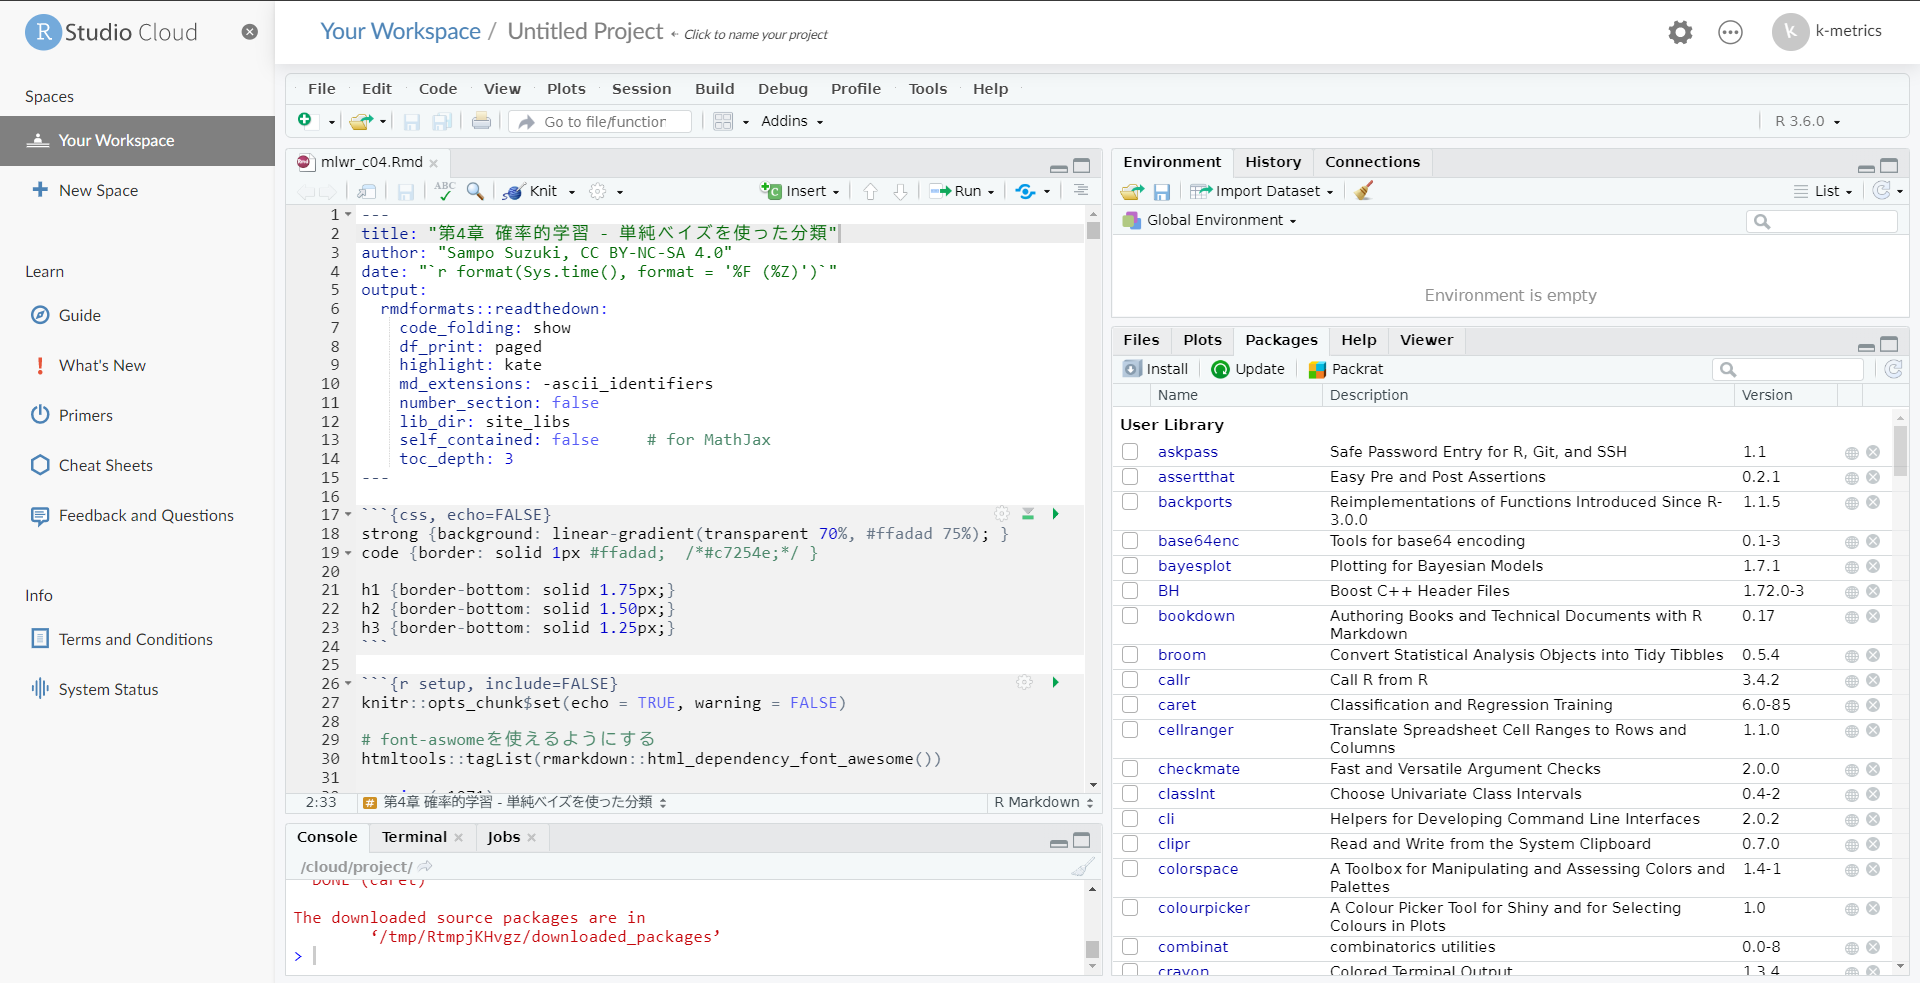
\includegraphics[width=0.8\linewidth,]{fig/RStudio/Cloud} 

}

\caption{RStudio Cloud, beta}\label{fig:unnamed-chunk-147}
\end{figure}

 

 ただし、無料プランで使えるリソースはメモリ 1GB ・ 1CPU と限られていますので、ナイーブ・ベイズのようなメモリを必要とする機械学習プログラミングなどには向いていません。なお、 Google Colab のように24時間でインスタンスが消滅するというようなことは無いようです。

 

\hypertarget{exploratory}{%
\section{Exploratory}\label{exploratory}}

 \href{https://exploratory.io/}{Exploratory } は BI(Business Intelligence)BI(Business Intelligence)ツールのような操作で R を持ちた探索的データ分析(EDA)が行える利用できる専用クライアントアプリケーションを用いるクラウドサービスです。無料で利用できますがオンライン限定・パブリックシェアオンリーとなりますので注意してください。

 \href{https://exploratory.io/insight?type=note\&q=tag\%3Avisualization\%20tag\%3Ahow-to\%20tag\%3A\%22team\%20exploratory\%22\&sort=top-viewed\&language=ja}{何ができるのか見てみる } ページで多数の分析サンプルが公開されています。\\
 また、 \href{https://exploratory.io/howto?language=ja}{使い方ガイド } ページにも様々な説明資料が用意されています。

 \\

\begin{figure}[H]

{\centering 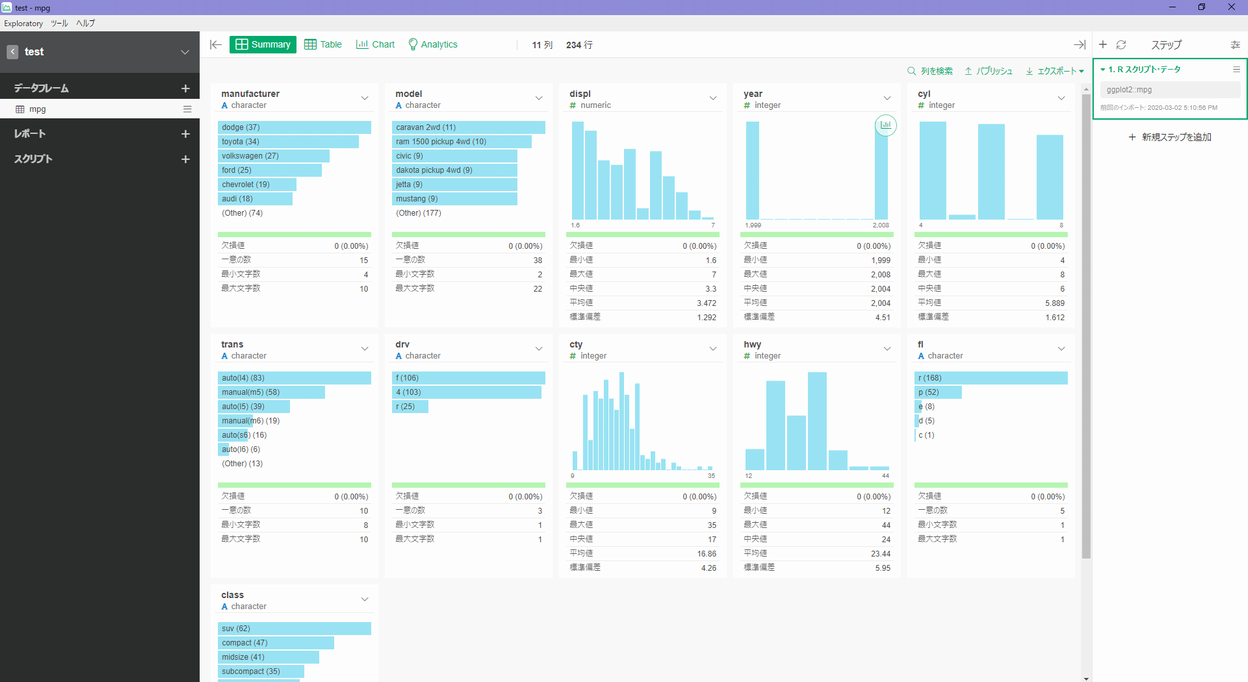
\includegraphics[width=0.8\linewidth,]{fig/Exploratory} 

}

\caption{Exploratory Public}\label{fig:unnamed-chunk-148}
\end{figure}

 

 \href{https://exploratory.io/pricing}{価格 } ページからお好みのプランを選んでアカウントを取得します。クライアントアプリケーションは、mac まはた Windwos でしか動作しません。

 

\hypertarget{binder}{%
\section{binder}\label{binder}}

 \href{https://mybinder.org/}{binder } は 実行環境の再現性を確保するためのクラウドサービスです。指定したGit のリポジトリから自動的に Jupyter Notebook のコード実行環境(Docker イメージ)を構築しクラウド上で実行することによりリポジトリにあるソースコードを動作さあせることができます。リポジトリに設定ファイルを置くことで RStudio Server や Shiny 環境を構築・実行することも可能です。\\
 Google Colab や RStudio Cloud・Exploratoy などと異なりアカウントを取得する必要はありませんが、専用の環境を構築するわけではなく、あくまでも一時的な試用環境である点に注意してください。継続的に使える環境が必要な場合は ローカルに環境を構築するか RStudio Cloud のようなクラウドサービスを利用してください。

 

  \bibliography{bib/references.bib,bib/packages.bib}

% --- Index(索引一覧)を作成する(ページがずれるバグあり)
% \cleardoublepage
% \phantomsection
% \printindex       % can be used to include the sorted and formatted index in the document.
% \see              % can used in the index to cross reference to other items.

% \cleardoublepage
% \phantomsection
% % \clearpage
% \vspace*{\stretch{1}}
% \begin{flushright}
% \begin{minipage}{0.5\hsize}
% \begin{description}
%   \item{著者:} Sampo Suzuki
%   % \item{表紙:} ASDF
%   \item{発行:} 2021年月日
%   % \item{サークル名:} ASDF
%   % \item{連絡先:} ASDF
%   % \item{印刷:} ASDF
% \end{description}
% \end{minipage}
% \end{flushright}
% \cleardoublepage
% % \clearpage

\end{document}
